\chapter{Experiments}\label{chap:experiments}
During this thesis several experiments were performed in order to evaluate the performance of the framework. We did different tests of all the parts of the modules, both in simulation and in the real world, in order to understand the weakness of each module and achieve better results.\\

In this chapter we describe the hardware used in the real world, the simulation environment and we report the main results achieved during these experiments.\\
%The system developed, utilize the Robot Operating System (ROS) [19]

\section{Real world hardware}
\subsection{Quadrotor}
We utilize custom-designed quadrotors that are based on 3D printed and electronic parts designed in the RPG lab, combined with some commercial components \ref{fig:quad_hardware}.\\
These platforms are lightweight ($\tilde500$ grams) and safe for operation in close proximity with humans. However, they are also agile while maintaining maneuverability and robust vision-based control: they can achieve a maximum speed of at least 4 m/s during vision-based flight.\\
The quadrotor used is equipped with:
\begin{itemize}
\item an inertial measurement unit (IMU) that reports linear accelerations and angular rates
\item a quad-core single board computer (Odroid XU4), where all computations described in the previous chapters are performed.
\item two different cameras:
\begin{itemize}
\item a down looking regular camera, used to detect and tracking the moving platform
\item a forward looking camera with fish eye lens, used for the quad self state estimation. The fish eye is used in order to have a bigger field of view and be able to track enough features in every configuration.
\end{itemize}
\end{itemize}
TODO PHOTO
\begin{figure}[!ht]
    \centering
    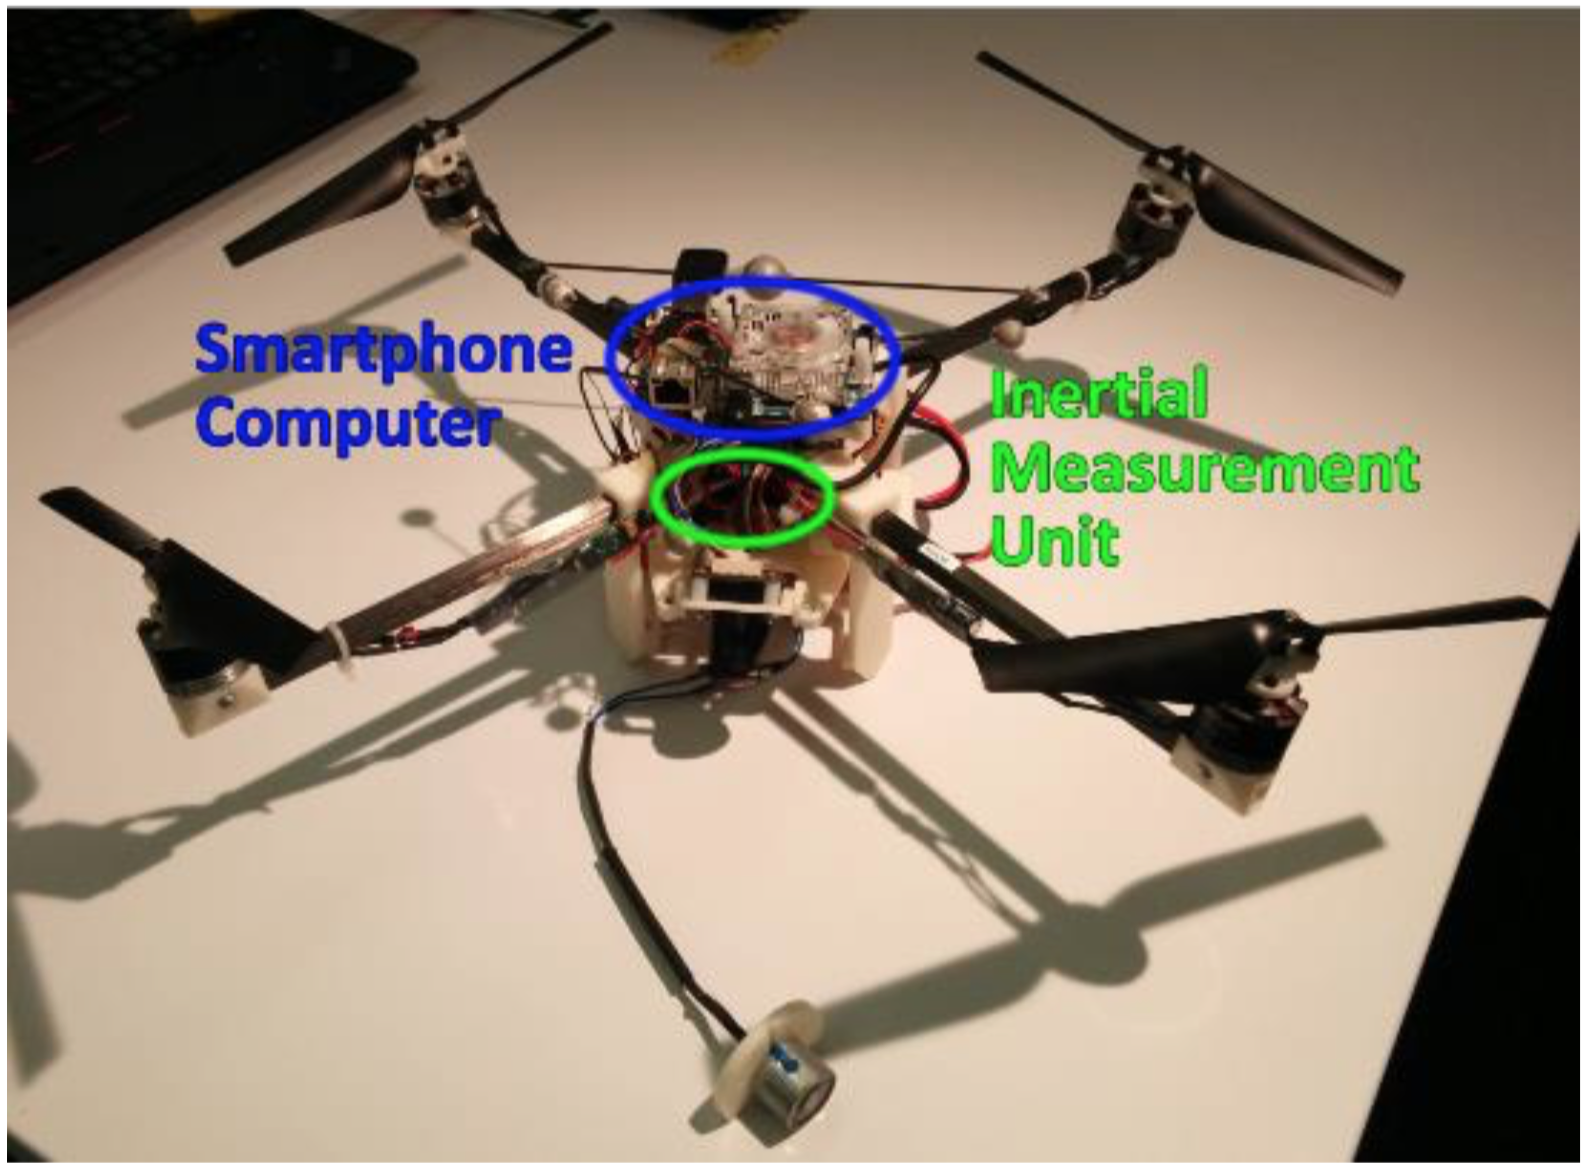
\includegraphics[width=0.65\textwidth]{img/photo_quad.png}
    \caption{The UAV used during the experiments}
    \label{fig:quad_hardware}
\end{figure}

\subsection{Moving platform}
During the experiments we are using Jackal UGV as moving platform.\\ 
Jackal is a small field robotics research platform produced by Clearpath Robotics \cite{clearpathrobotics}. It has an onboard computer, GPS, IMU and it is fully integrated with ROS.\\
It can reach a maximum speed of $2m/s$ that is perfect for testing with condition similar to the final challenge.\\
Over the UGV we have installed a wooden base $1m \times 1m$ were we can attached both the textures     \ref{fig:finalplatform} or \ref{fig:tempplatform}.
\begin{figure}[!ht]
    \centering
    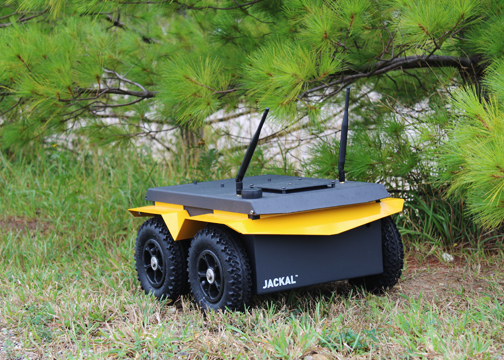
\includegraphics[width=0.65\textwidth]{img/jackal.jpg}
    \caption{The UGV used during the experiments}
    \label{fig:quad_hardware}
\end{figure}

\section{Simulation}
A simulation environment is developed in order to recreate as precise as possible the final environment of the challenge.  As a matter of fact, organizing experiments in real field as large as the one in the challenge, can be difficult, but with the simulation environment we can test the whole framework before trying it in the real world.\\

The simulation is done using Gazebo simulator \cite{gazebosimulator}: a free simulation toolbox useful to reproduce populations of robots in complex indoor and outdoor environments, furthermore this toolbox is directly part of ROS.\\
To simulate the quadrotor we are using RotorS simulator \cite{rotors2016}: a UAV gazebo simulator that provides some multirotor models among which there is the AscTec Hummingbird, very similar to the quadrotor we are using in the real world experiments. All quadrotor can be provided with many sensors such as IMU, cameras etc. \\
To simulate the moving platform we are using the ROS package \cite{RobotsHusky} that allow to control a Clearpath Husky. Over the UGV we installed a platform identical to the one used in the real world.\\

The framework used during the tests in the simulation are the same w.r.t. the one explained in chapter \ref{chap:general_framework}, with the difference that the state estimation is not coming from SVO+MSF, but is given by Gazebo and we corrupted it with a Gaussian noise with 0 mean and $\sigma^2$ variance.

\begin{figure}[!ht]
    \centering
    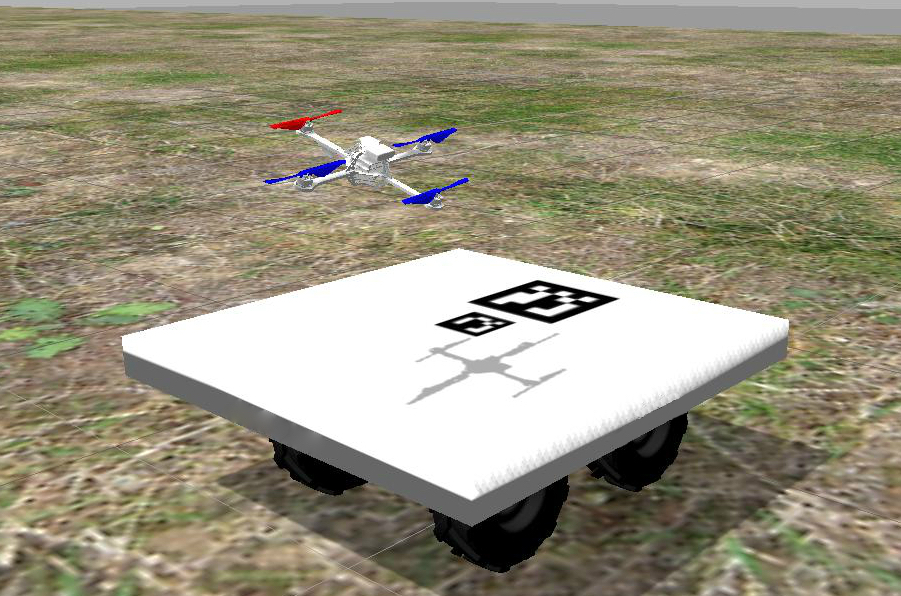
\includegraphics[width=0.7\textwidth]{img/simulation.jpg}
    \caption{The UAV and UGV used during the experiments in simulation}
    \label{fig:quad_ugv_sim}
\end{figure}

\section{SVO}
For this project we need to use a front looking camera for the visual odometry, because, when the UAV is over the base, the majority of the image from the down looking camera is occluded by the platform itself.\\
This is a crucial problem because the features on the base cannot be considered: the perceived movement is relative to the moving platform and not to the world frame. For example in the scenario in which the quadrotor and the platform are moving with the same velocity, the images taken from the camera are not changing over time, even if the camera is moving. In this case the visual odometry fails.\\
In the final parts of the framework,using the down looking camera, there will be not enough good features to track  for UAV state estimation, so is necessary to use a front looking camera for self state estimation.

\subsection{Front looking vs down looking}
To compare the results of front looking and down looking SVO we have taken data sets in which we are running two instances of SVO (using the two different images from the two cameras) to compute the pose estimation of the quadrotor and then filter these pose with MSF using the same IMU signal. \\
These state estimations are compared also with the ground truth from the optitrack motion capture system \cite{optitrack}. In this way we can compare the 2 versions of SVO+MSF with the real pose.\\

The following images show the the results of one of these experiments. In this particular test we were holding the quadrotor by hand and we were moving inside the flyingroom simulating a square trajectory \ref{fig:comparision_svo_trajectory}.\\
In particular the first images show the position \ref{fig:comparision_svo_position}, the orientation  \ref{fig:comparision_svo_angles} and the velocity \ref{fig:comparision_svo_velocities} estimations from the two versions of SVO compared with the optitrack.
 
\begin{figure}[!ht]
    \centering
    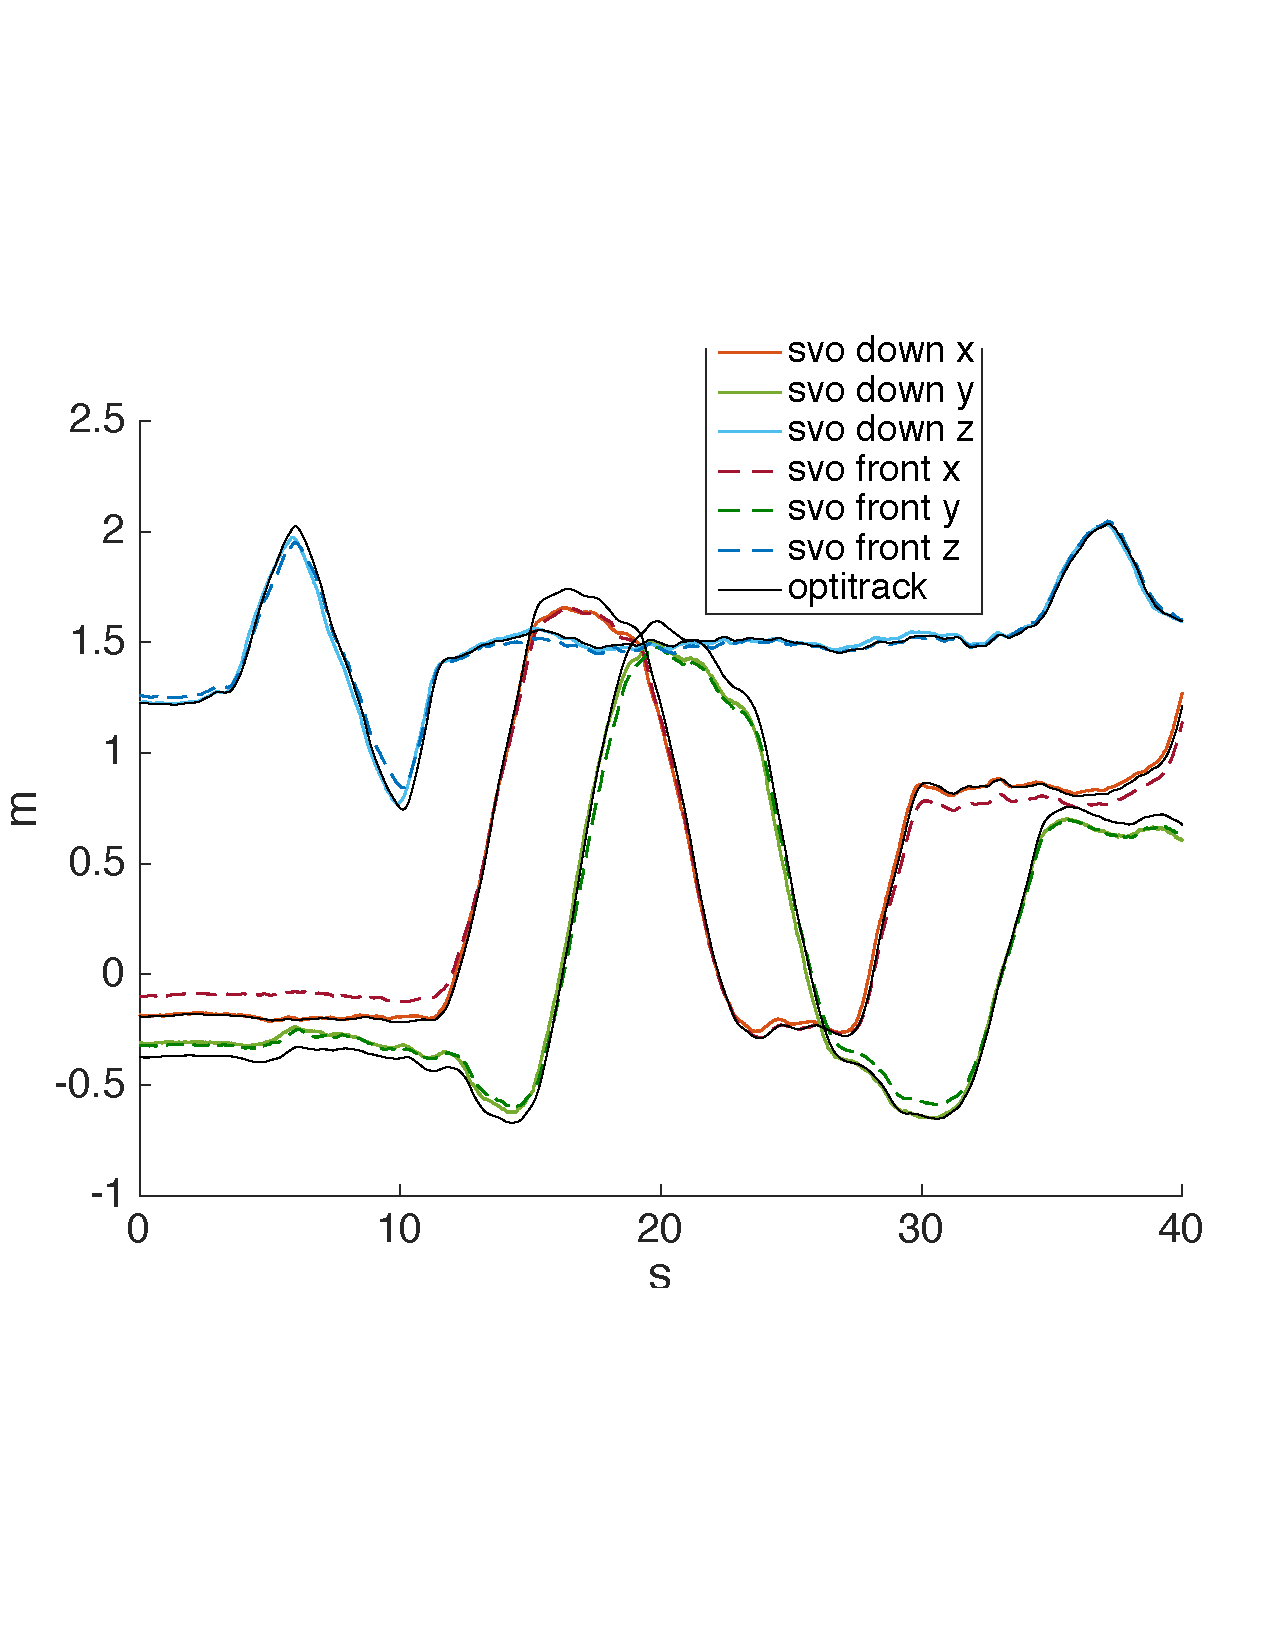
\includegraphics[width=0.75\textwidth]{img/comparision_between_two_svo_and_opti_position.pdf}
    \caption{Comparison between SVO position estimations with the front looking camera (dashed lines), down looking camera (solid) and optitrack (black) }
    \label{fig:comparision_svo_position}
\end{figure}

\begin{figure}[!ht]
    \centering
    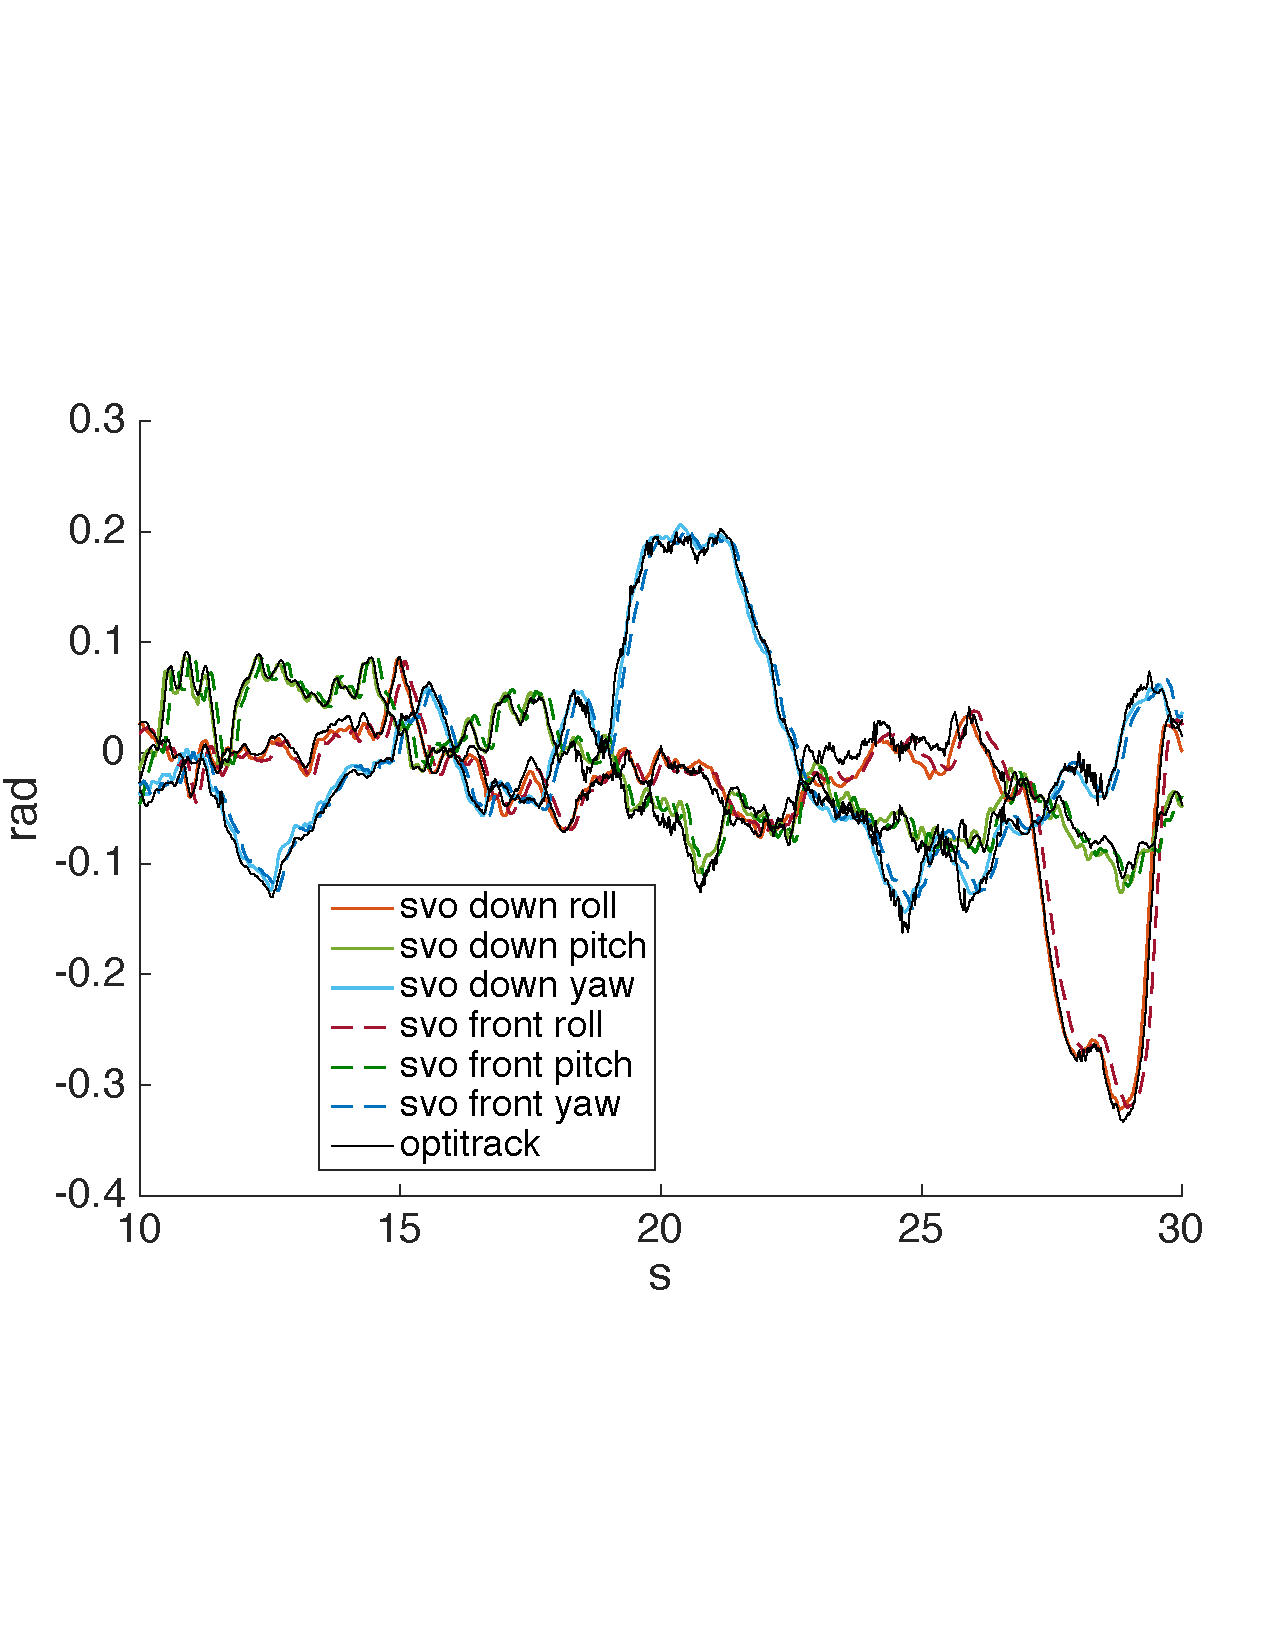
\includegraphics[width=0.75\textwidth]{img/comparision_between_two_svo_and_opti_angles.pdf}
    \caption{Comparison between SVO orientation estimations with the front looking camera (dashed lines), down looking camera (solid lines) , and optitrack (black lines). The orientation data from the optitrack are low pass filtered in order to eliminate the high frequency noise. }
    \label{fig:comparision_svo_angles}
\end{figure}

\begin{figure}[!ht]
    \centering
    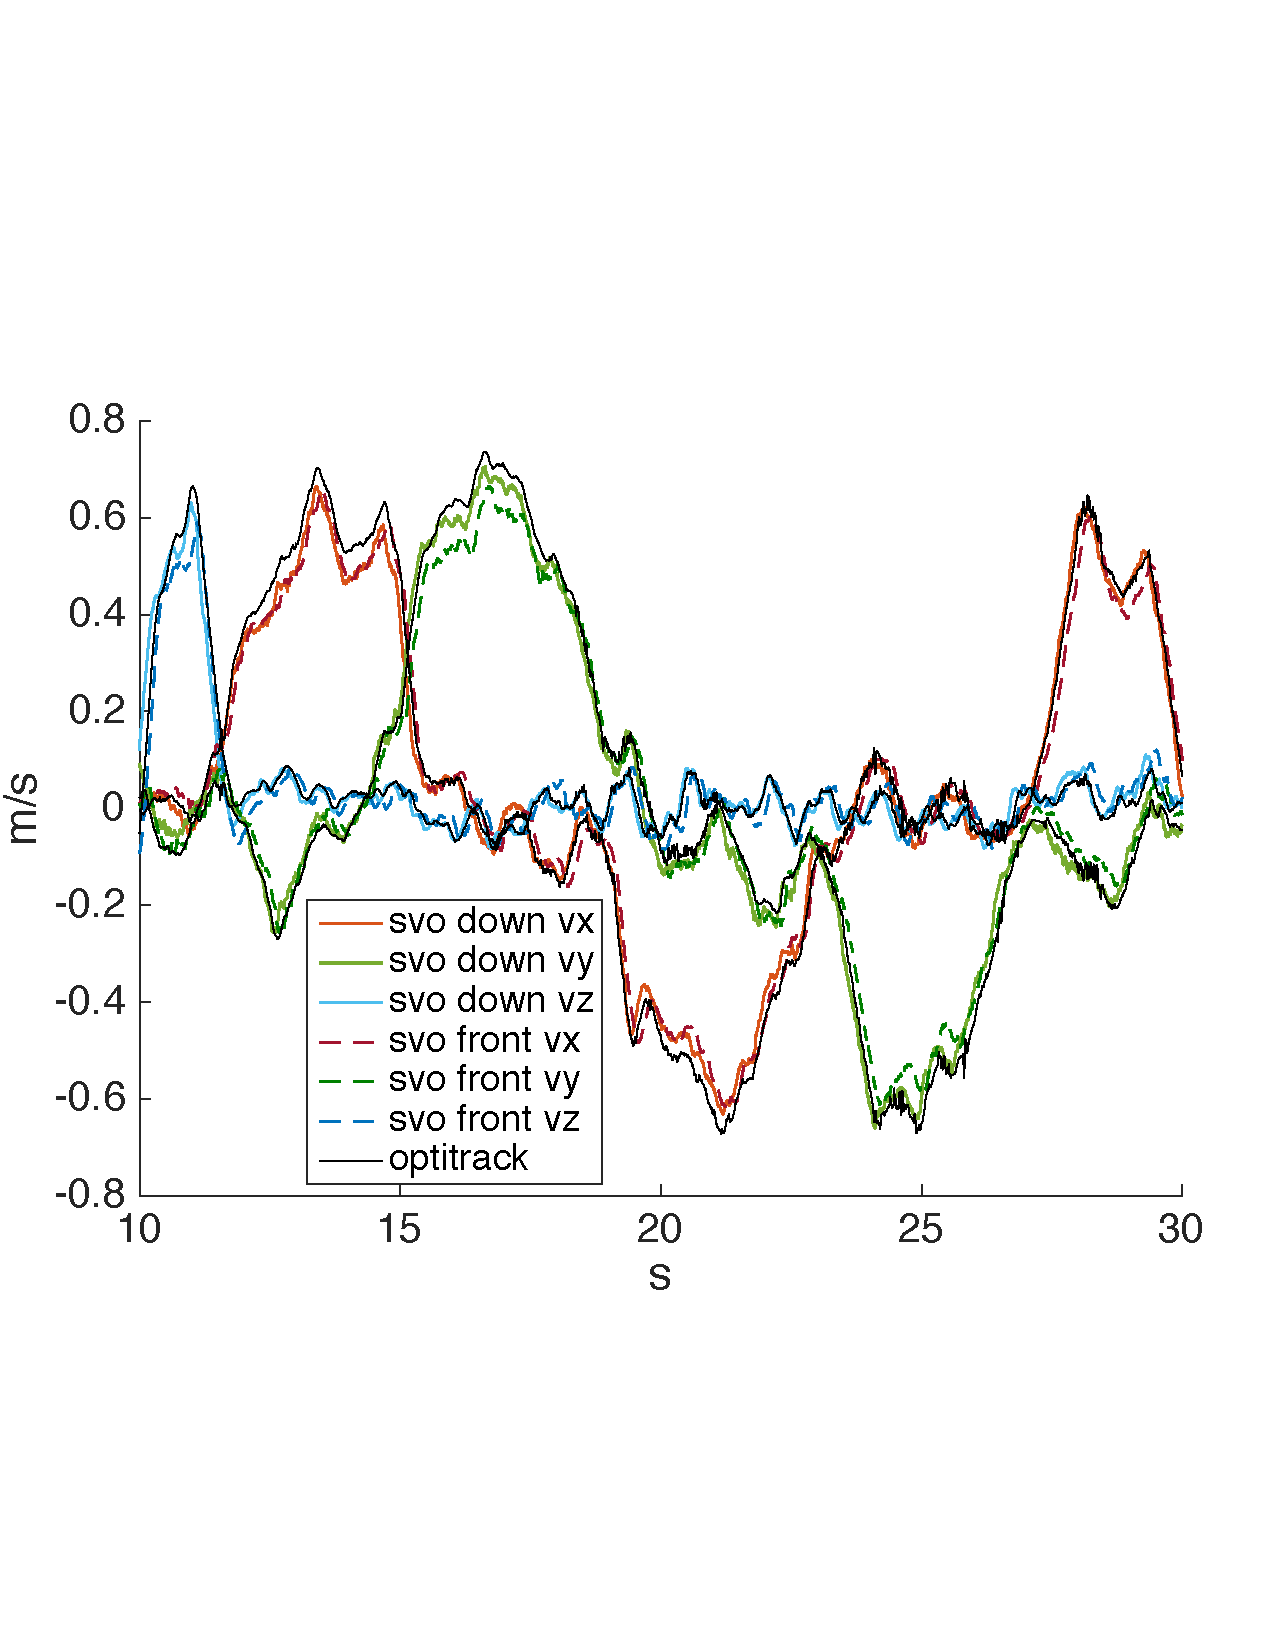
\includegraphics[width=0.75\textwidth]{img/comparision_between_two_svo_and_opti_velocities.pdf}
    \caption{Comparison between SVO position estimations with the front looking camera (dashed lines), down looking camera (solid lines), and optitrack (black lines). The velocity data from the optitrack are low pass filtered in order to eliminate the high frequency noise.  }
    \label{fig:comparision_svo_velocities}
\end{figure}

We can see that both the versions of our estimation framework are calculating a reliable estimation of the quadrotor pose and velocity. In order to evaluate the precision of the two estimations, see figure \ref{fig:comparision_svo_error}. It shows the average position error between the two versions of SVO: error generally below $10cm$ with RMSE of $4.5cm$ for the down looking camera and $6cm$ for the front looking one.\\

\begin{figure}[!ht]
    \centering
    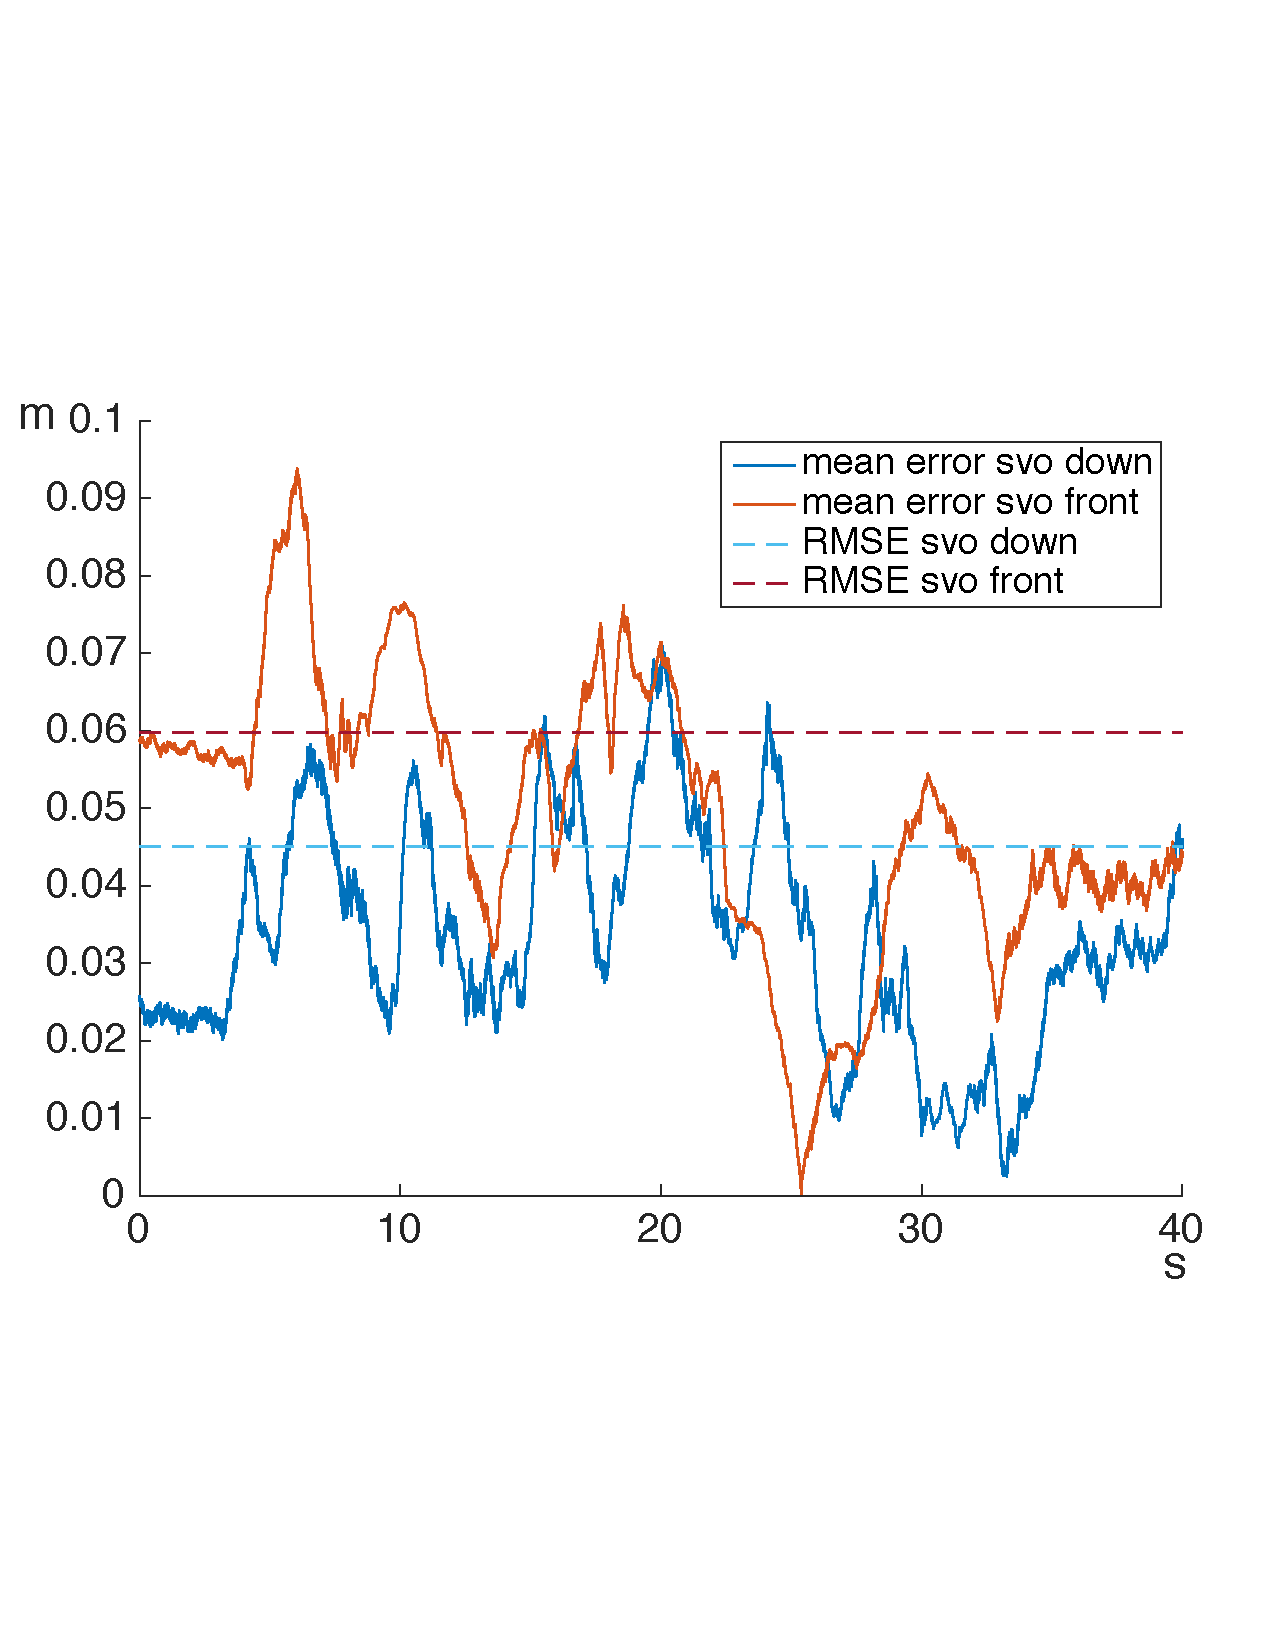
\includegraphics[width=0.7\textwidth]{img/comparision_between_two_svo_and_opti_error.pdf}
    \caption{Mean error between the 3D position estimations of the two versions of SVO and the ground truth. Blue line is the error with the down looking camera, the red line with the front looking one. The correspondent dashed lines are the RMSE for the two estimations.}
    \label{fig:comparision_svo_error}
\end{figure}

This error is larger then expected. In particular the graphs \ref{fig:perc_error} shows the percentage error of the position estimations, related to the maximum distance traveled in each direction. We can see that the error is below $6\%$ in $x,y$ and $8\%$ in $z$ that correspond to a general absolute error smaller than $10cm$.

\begin{figure}[!htbp]
  \centering
  \begin{subfigure}[b]{0.3\textwidth}
        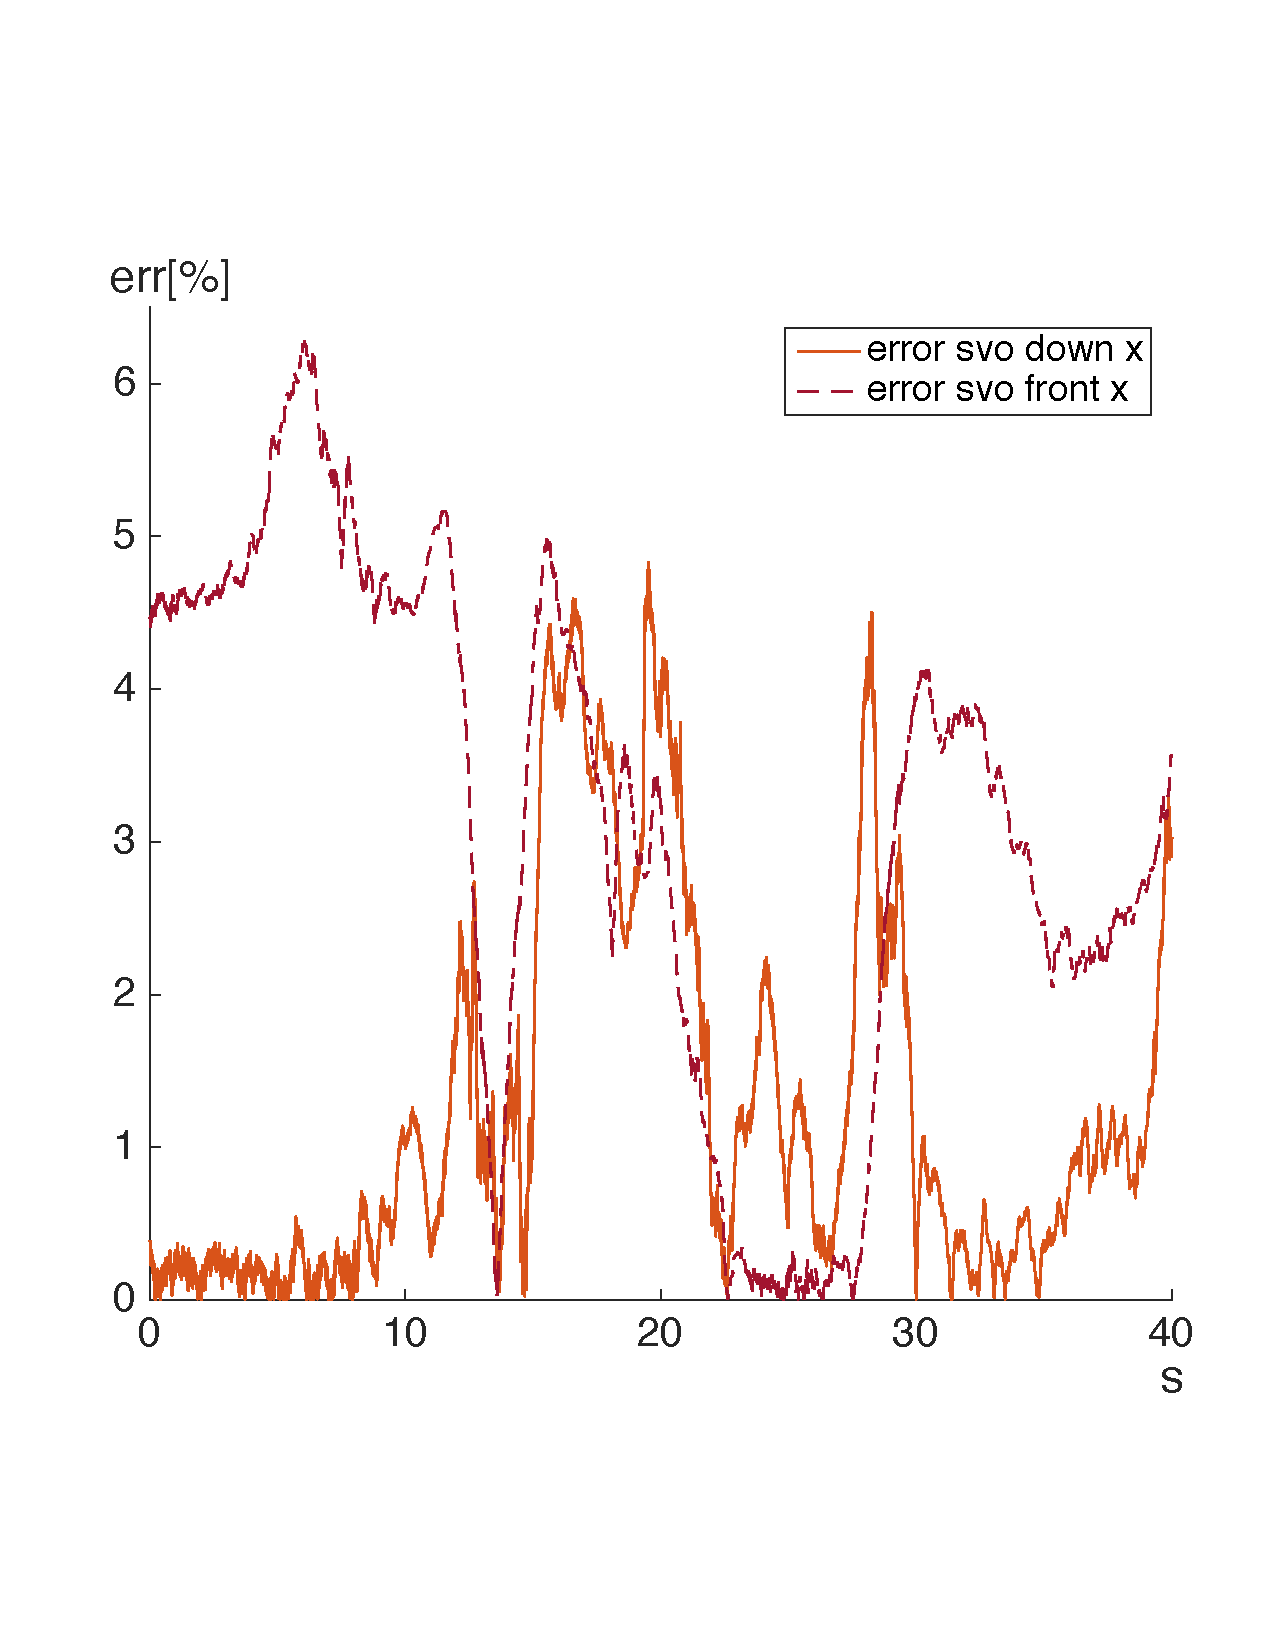
\includegraphics[width=\textwidth]{img/err_perc_2_svo_x.pdf}
        \label{fig:perc_errorone}
   \end{subfigure} \hfill
   \begin{subfigure}[b]{0.3\textwidth}
        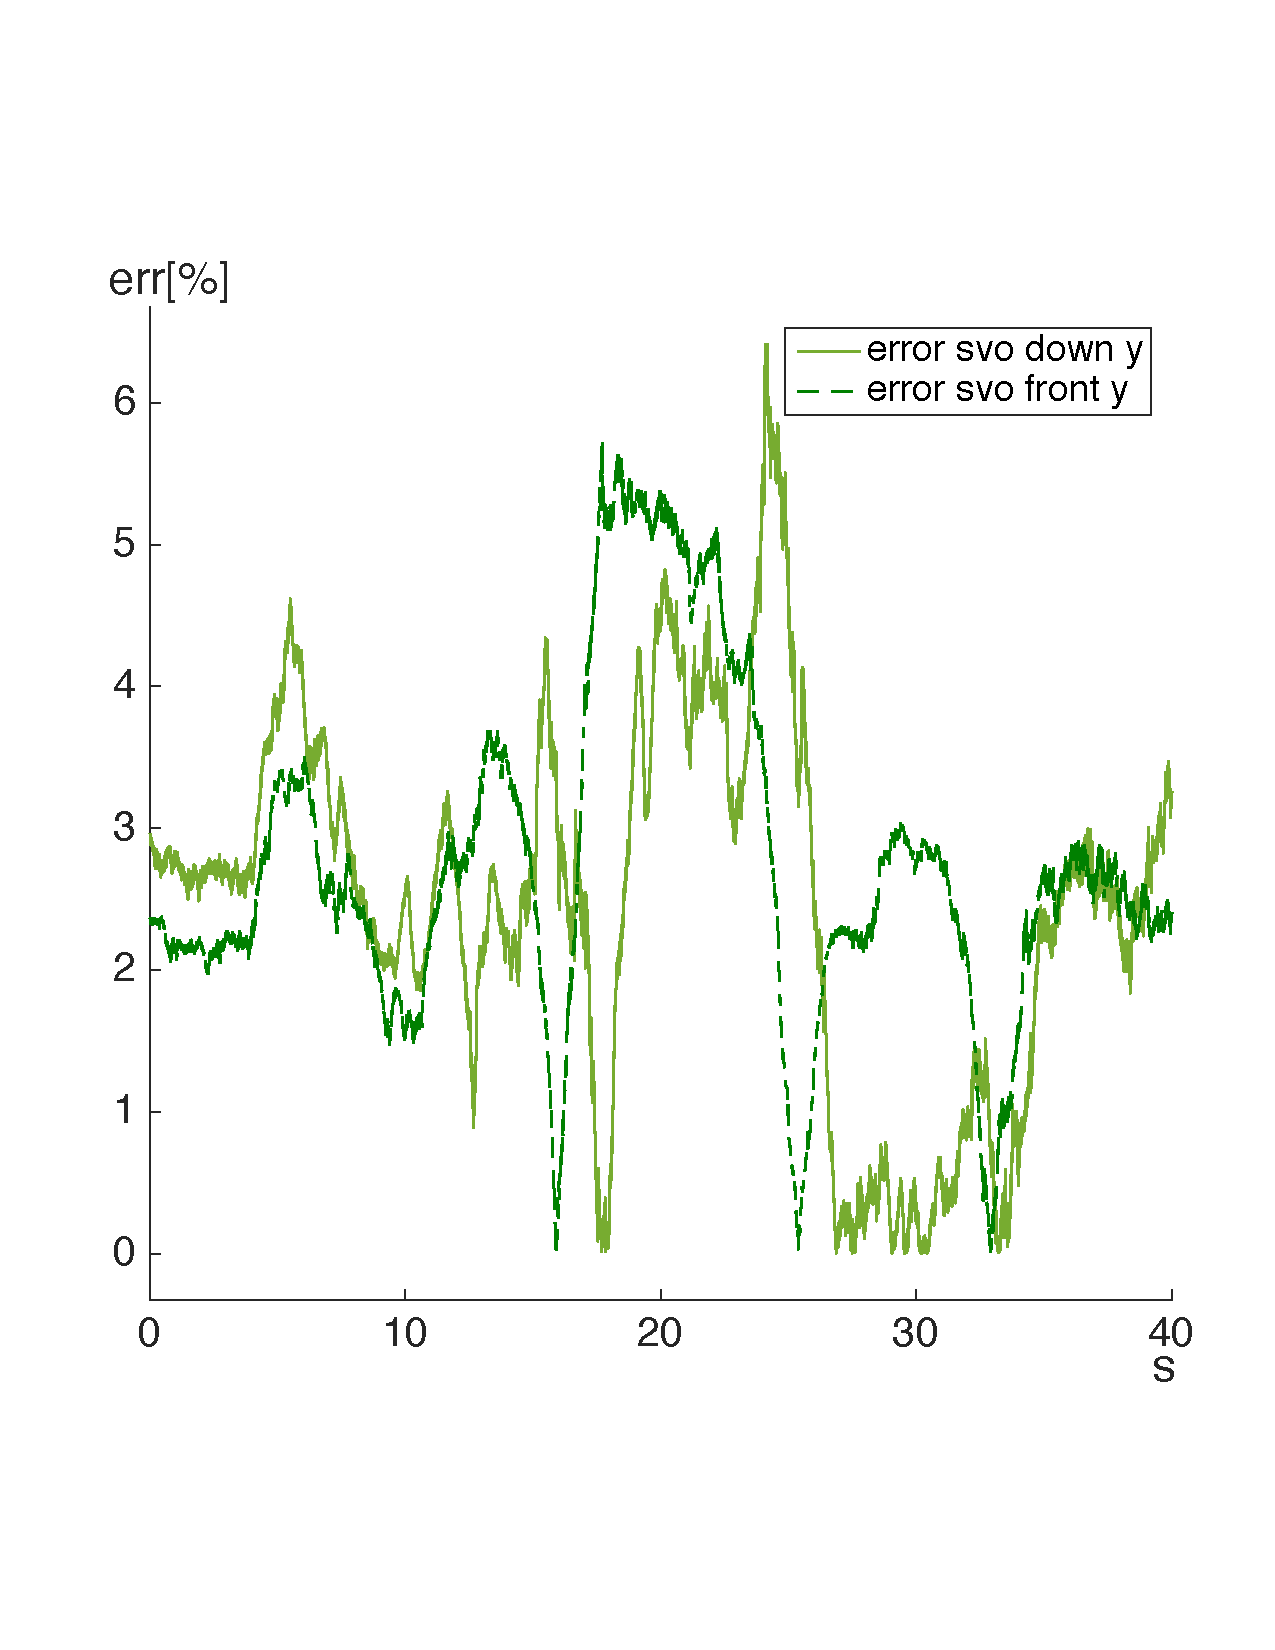
\includegraphics[width=\textwidth]{img/err_perc_2_svo_y.pdf}
        \label{fig:perc_errortwo}
   \end{subfigure}\hfill
   \begin{subfigure}[b]{0.3\textwidth}
        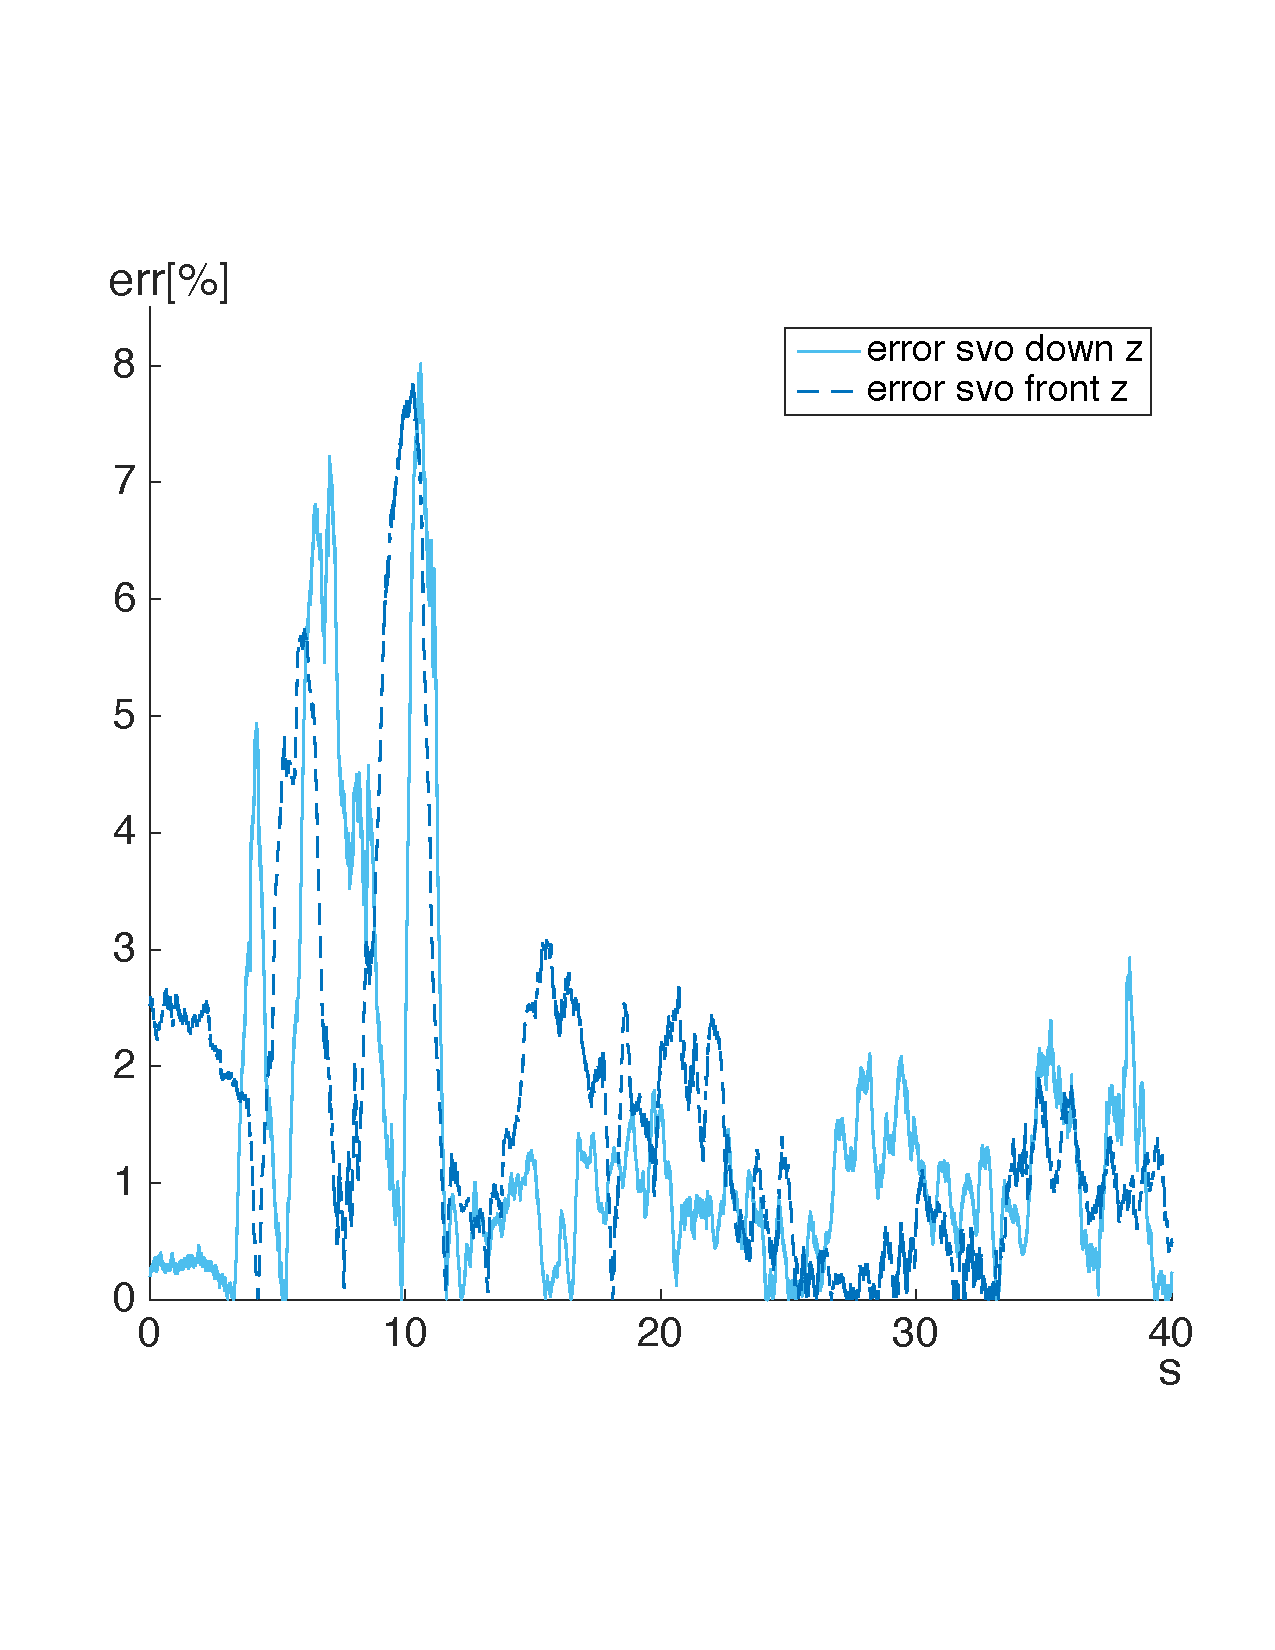
\includegraphics[width=\textwidth]{img/err_perc_2_svo_z.pdf}
        \label{fig:perc_errorthree}
   \end{subfigure}
  \caption{Percentage error, in each dimension, between the two version of SVO and the ground truth given by the optitrack. The quad traveled more or less 2m in x,y direction and 1m in z.}
  \label{fig:perc_error}
\end{figure} 

From the image of the 3D trajectory \ref{fig:comparision_svo_trajectory} we can see that the main problem is the scale factor, not drifting in the state estimation. The scale factor is estimated at the beginning, tracking features of the images and setting their depth using external means, other then the images (default depth or laser). If there is an error in this initialization then all the world is scaled and will result bigger or smaller then the reality.
\begin{figure}[!htbp]
    \centering
    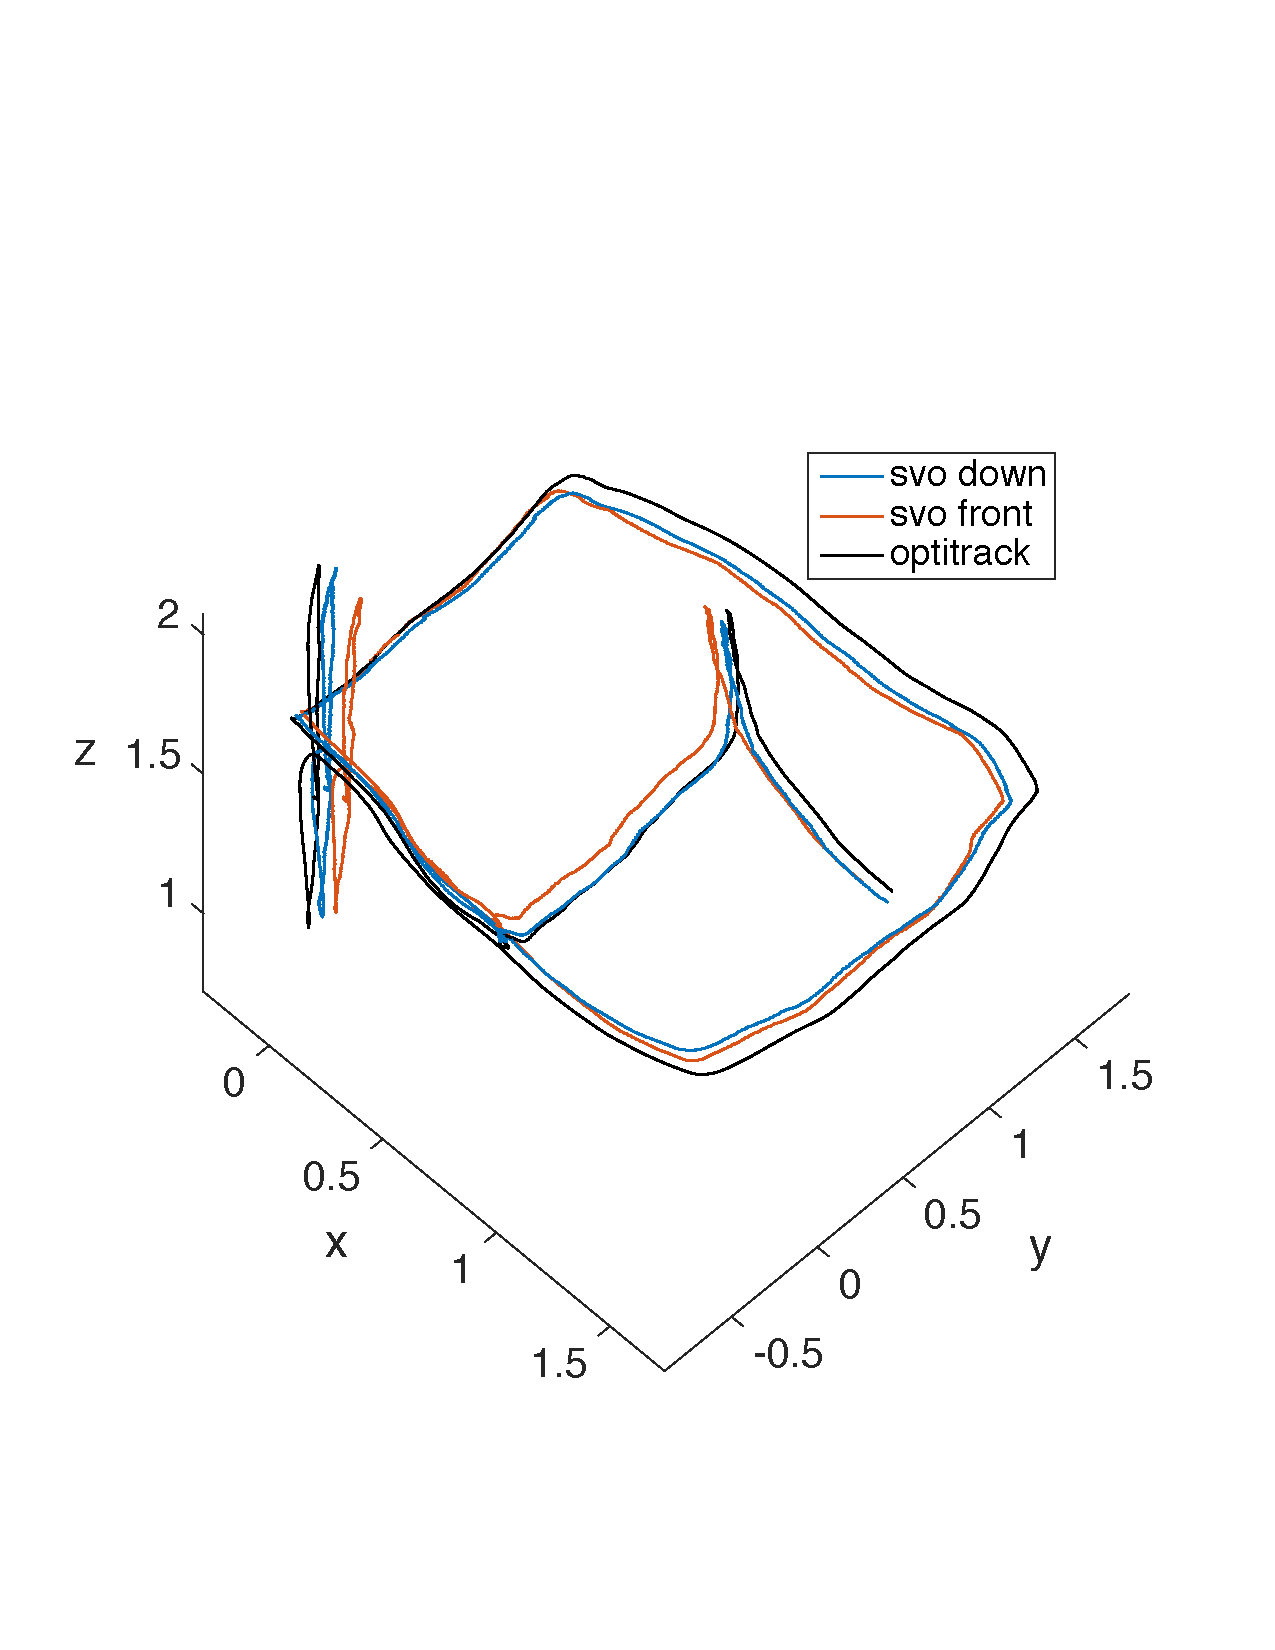
\includegraphics[width=0.7\textwidth]{img/comparision_between_two_svo_and_opti_trajectory.pdf}
    \caption{Comparison between SVO position estimation in 3D world. The blue line is the estimation with down looking camera, the red line with front looking one and the black line the ground truth given by the optitrack}
    \label{fig:comparision_svo_trajectory}
\end{figure}

\subsection{Drifting}
We made other experiments to understand if the current version of frontlooking-fisheye-SVO is good enough to fly with it.\\ 
We performed several manual flights in the flyingroom, with the same results: generally SVO is estimating a correct and precise state of the quad, but sometimes it occurs that the state estimation is drifting w.r.t the real world.\\
For example the data set showed in figure \ref{fig:svo_position_driftind} is related to a flight in which three times the SVO estimation drifted with respect to the real world in all three axes. We Highlighted in the figure these moments.\\

\begin{figure}[!htbp]
  \centering
  \begin{subfigure}[b]{0.4\textwidth}
        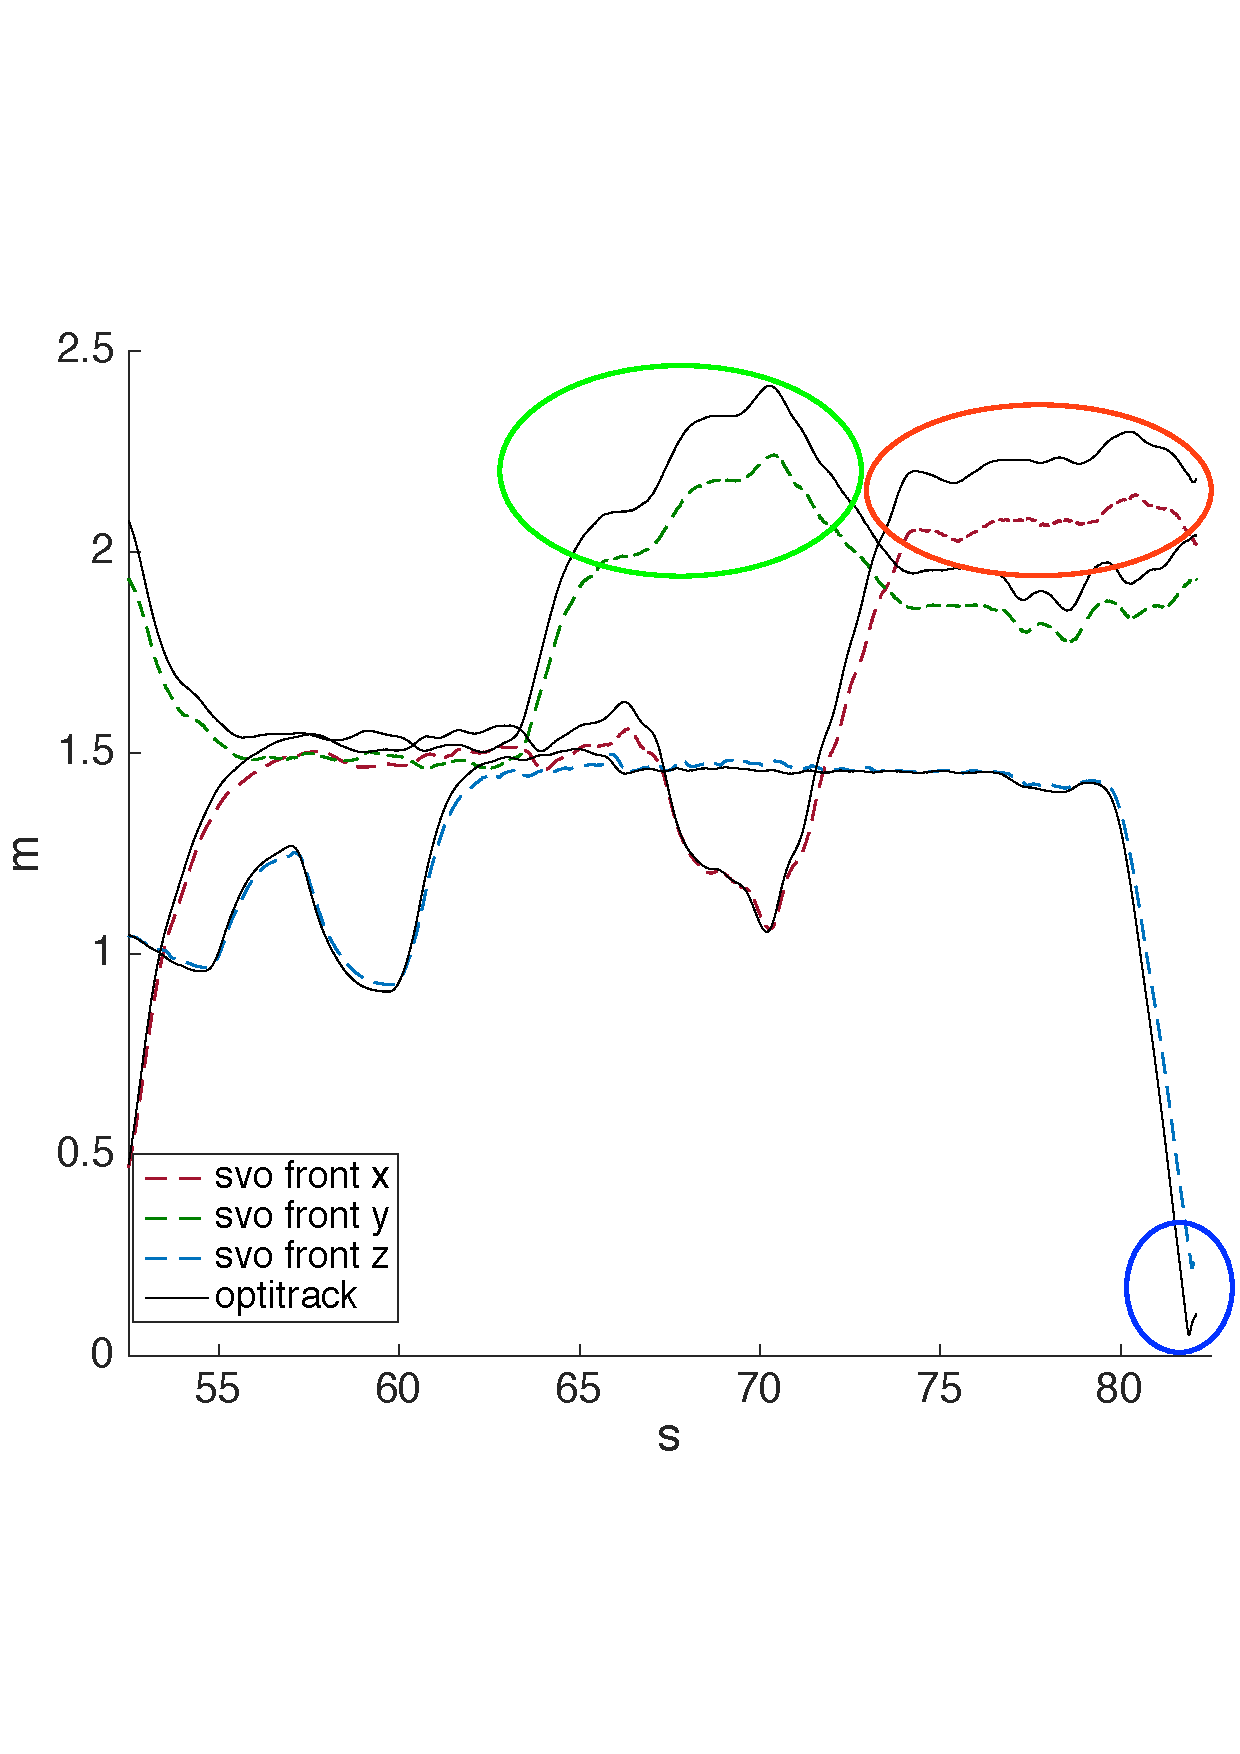
\includegraphics[width=\textwidth]{img/fly_with_landing_position.pdf}
        \label{fig:comparision_svo_position_drifting}
   \end{subfigure} \\
   \begin{subfigure}[b]{0.4\textwidth}
        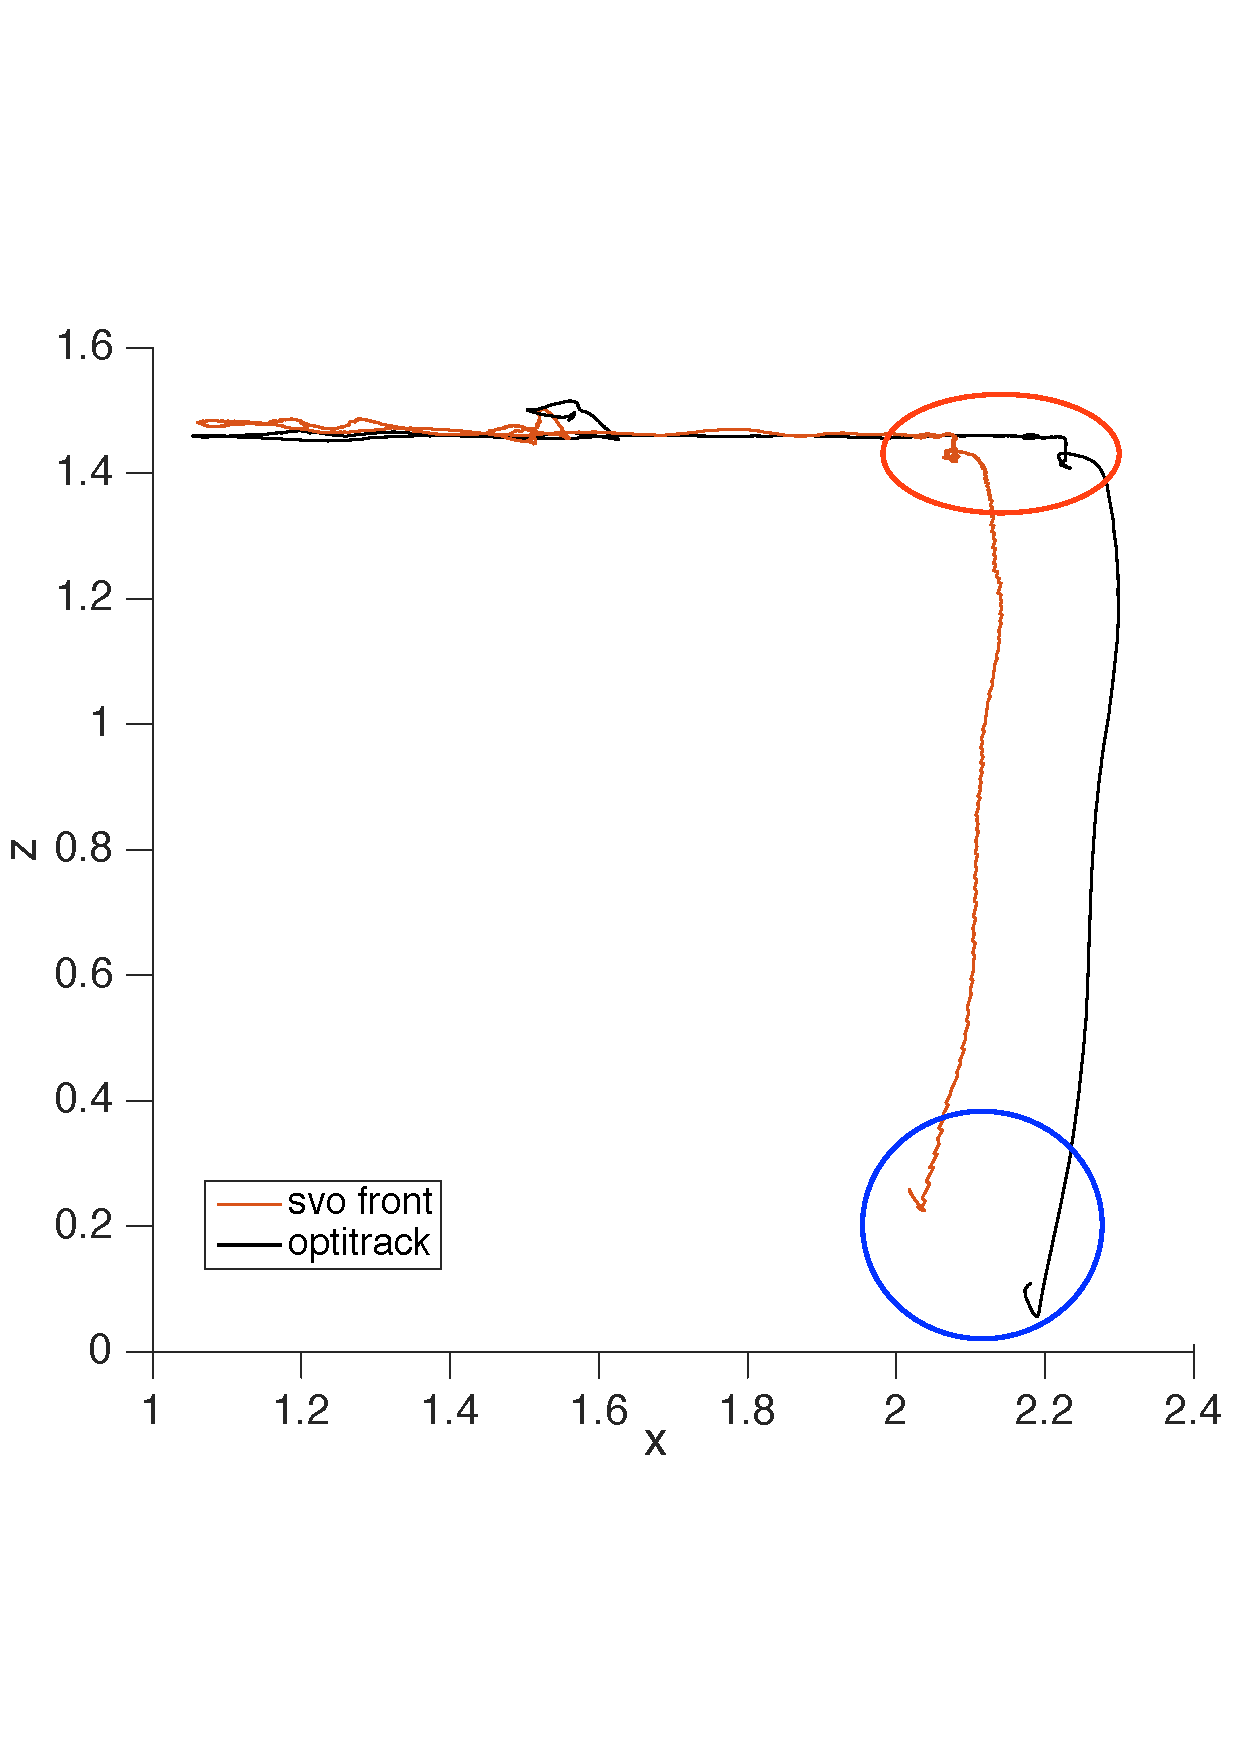
\includegraphics[width=\textwidth]{img/fly_with_landing_trajectory_x.pdf}
        \label{fig:comparision_svo_position_drifting_x}
   \end{subfigure}\hfill
   \begin{subfigure}[b]{0.4\textwidth}
        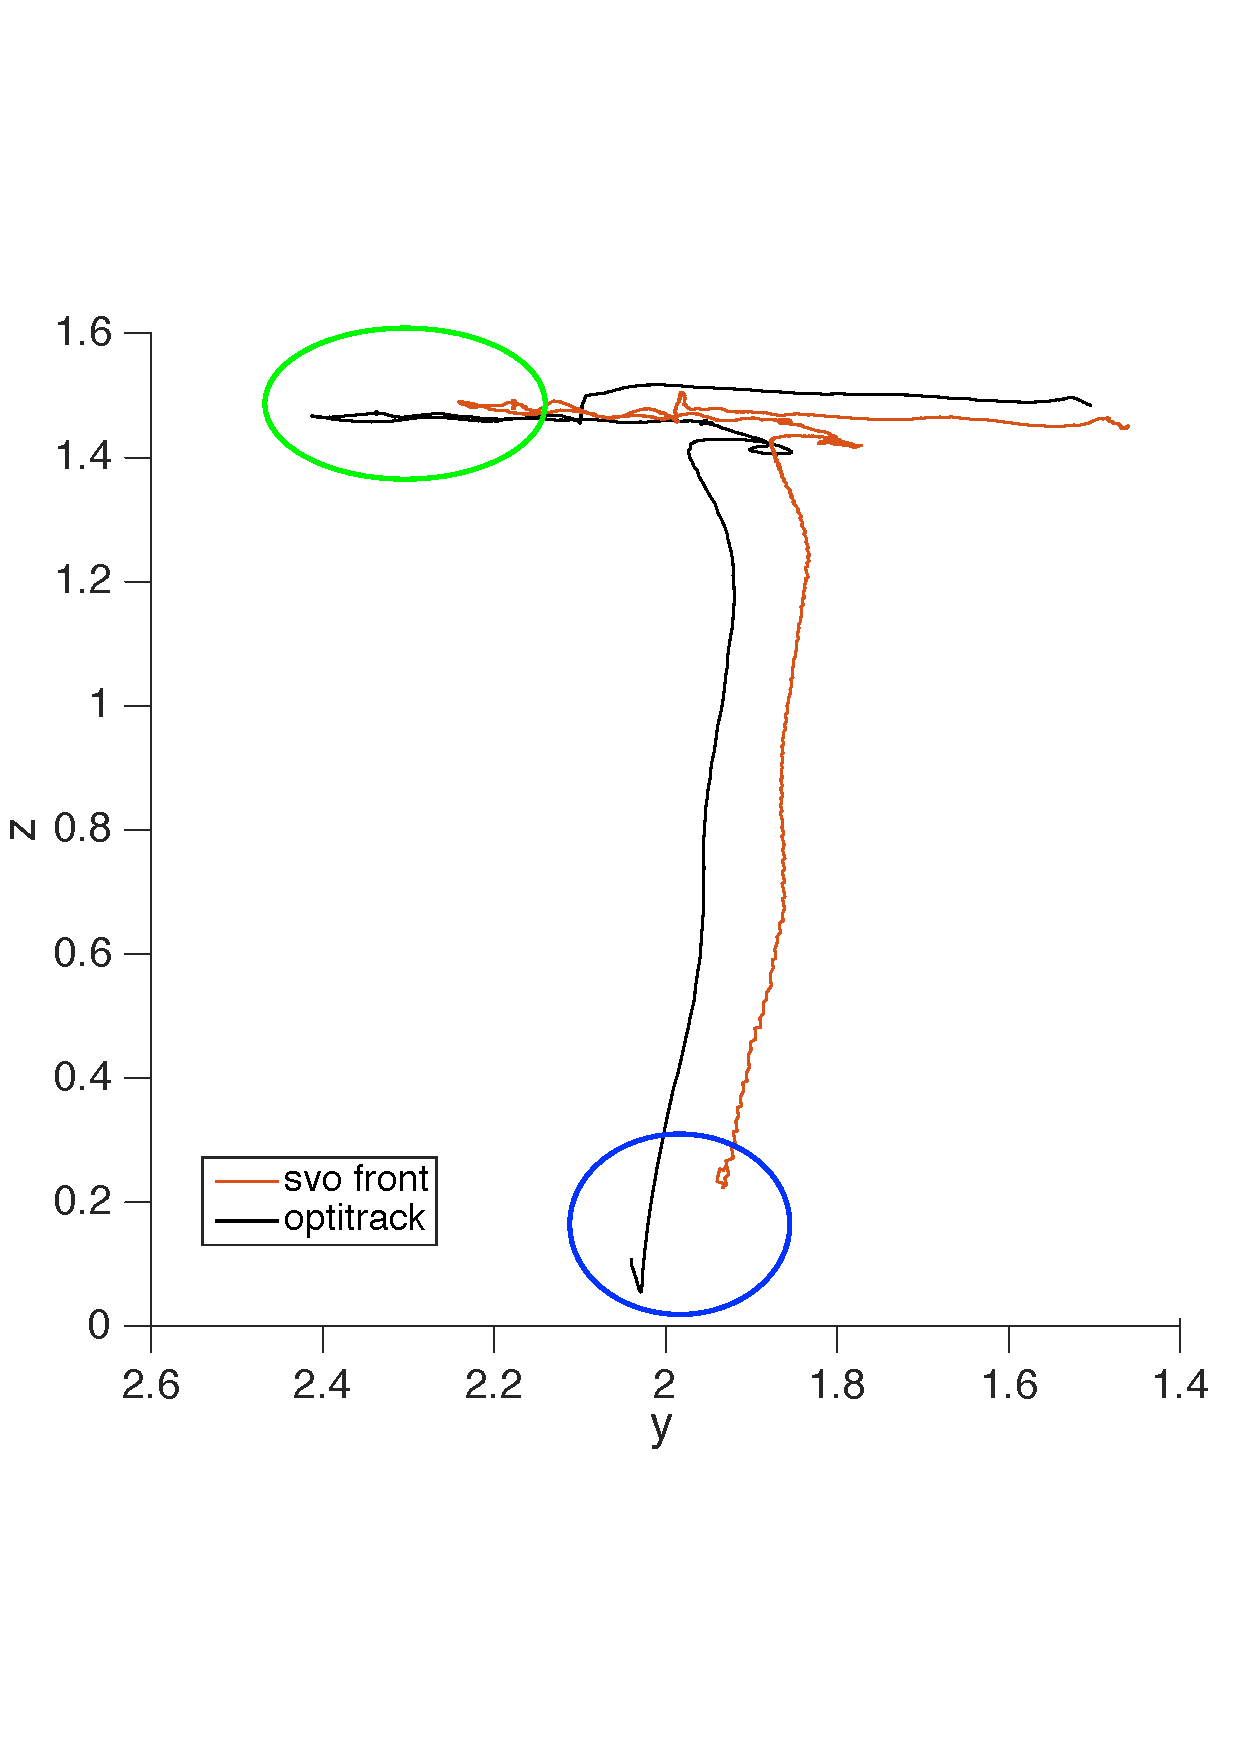
\includegraphics[width=\textwidth]{img/fly_with_landing_trajectory_y.pdf}
        \label{fig:comparision_svo_position_drifting_y}
   \end{subfigure}
  \caption{Manual flight in which SVO drifted away from the reality. Highlighted by circles are the moment in which these drifts happened and there are the correspondences between the time domain and the trajectory. }
  \label{fig:svo_position_driftind}
\end{figure} 

The reasons for this behavior can be related to the poverty of features that the vertical walls in the flyingroom has. As a matter of fact if there are no enough distinctive features the visual odometry can drift. TODO ???

\subsection{Very fast flight}
In the final challenge the moving car will move at $15\frac{km}{h}$ that means $4.17\frac{m}{s}$. IN order the quadrotor to be able to follow and land on the platform it must flight faster then this velocity.\\
We made some experiments to understand if the state estimation with the front looking camera it is precise at this high speed. TODO complete


\section{Base detection and tracking}
Several experiments were performed both in simulation and in the real world to evaluate the performance of the state estimation.
\subsection{From high altitude}
We are not requiring the state estimation from high altitude to be very precise, we need a rough estimation of the position of the platform, but it is important to be consistent and without lots of jumps.\\
The precision of the estimation is depending on the altitude from which the quadrotor is tracking the base, but anyway, with the designed  EKF we obtain a reliable estimation of the base state.\\
The following figures show the result of different experiments computed in simulation.

\begin{figure}[!htbp]
  \centering
  \begin{subfigure}[b]{0.6\textwidth}
        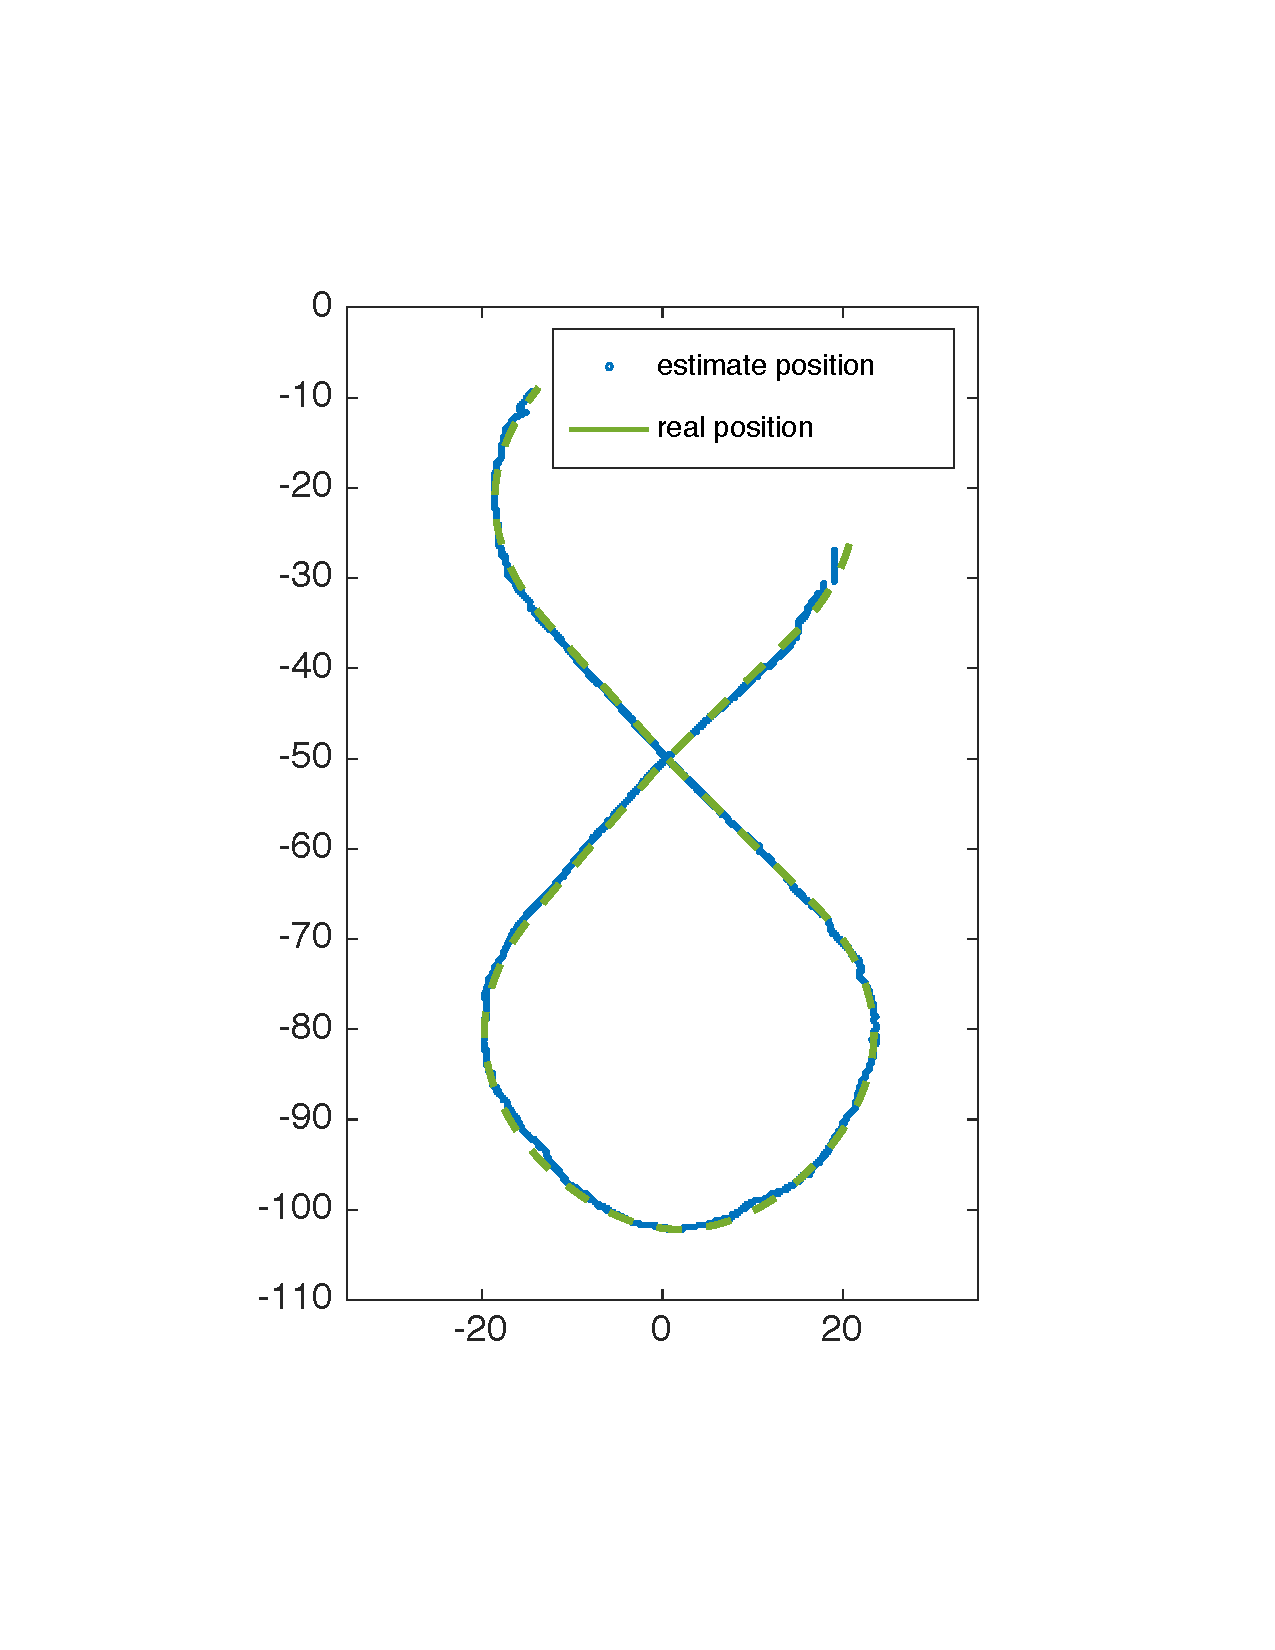
\includegraphics[width=\textwidth]{img/high_altitude_error_xy.pdf}
        \caption{Trajectory}
        \label{fig:one}
   \end{subfigure} \\
   \begin{subfigure}[b]{0.4\textwidth}
        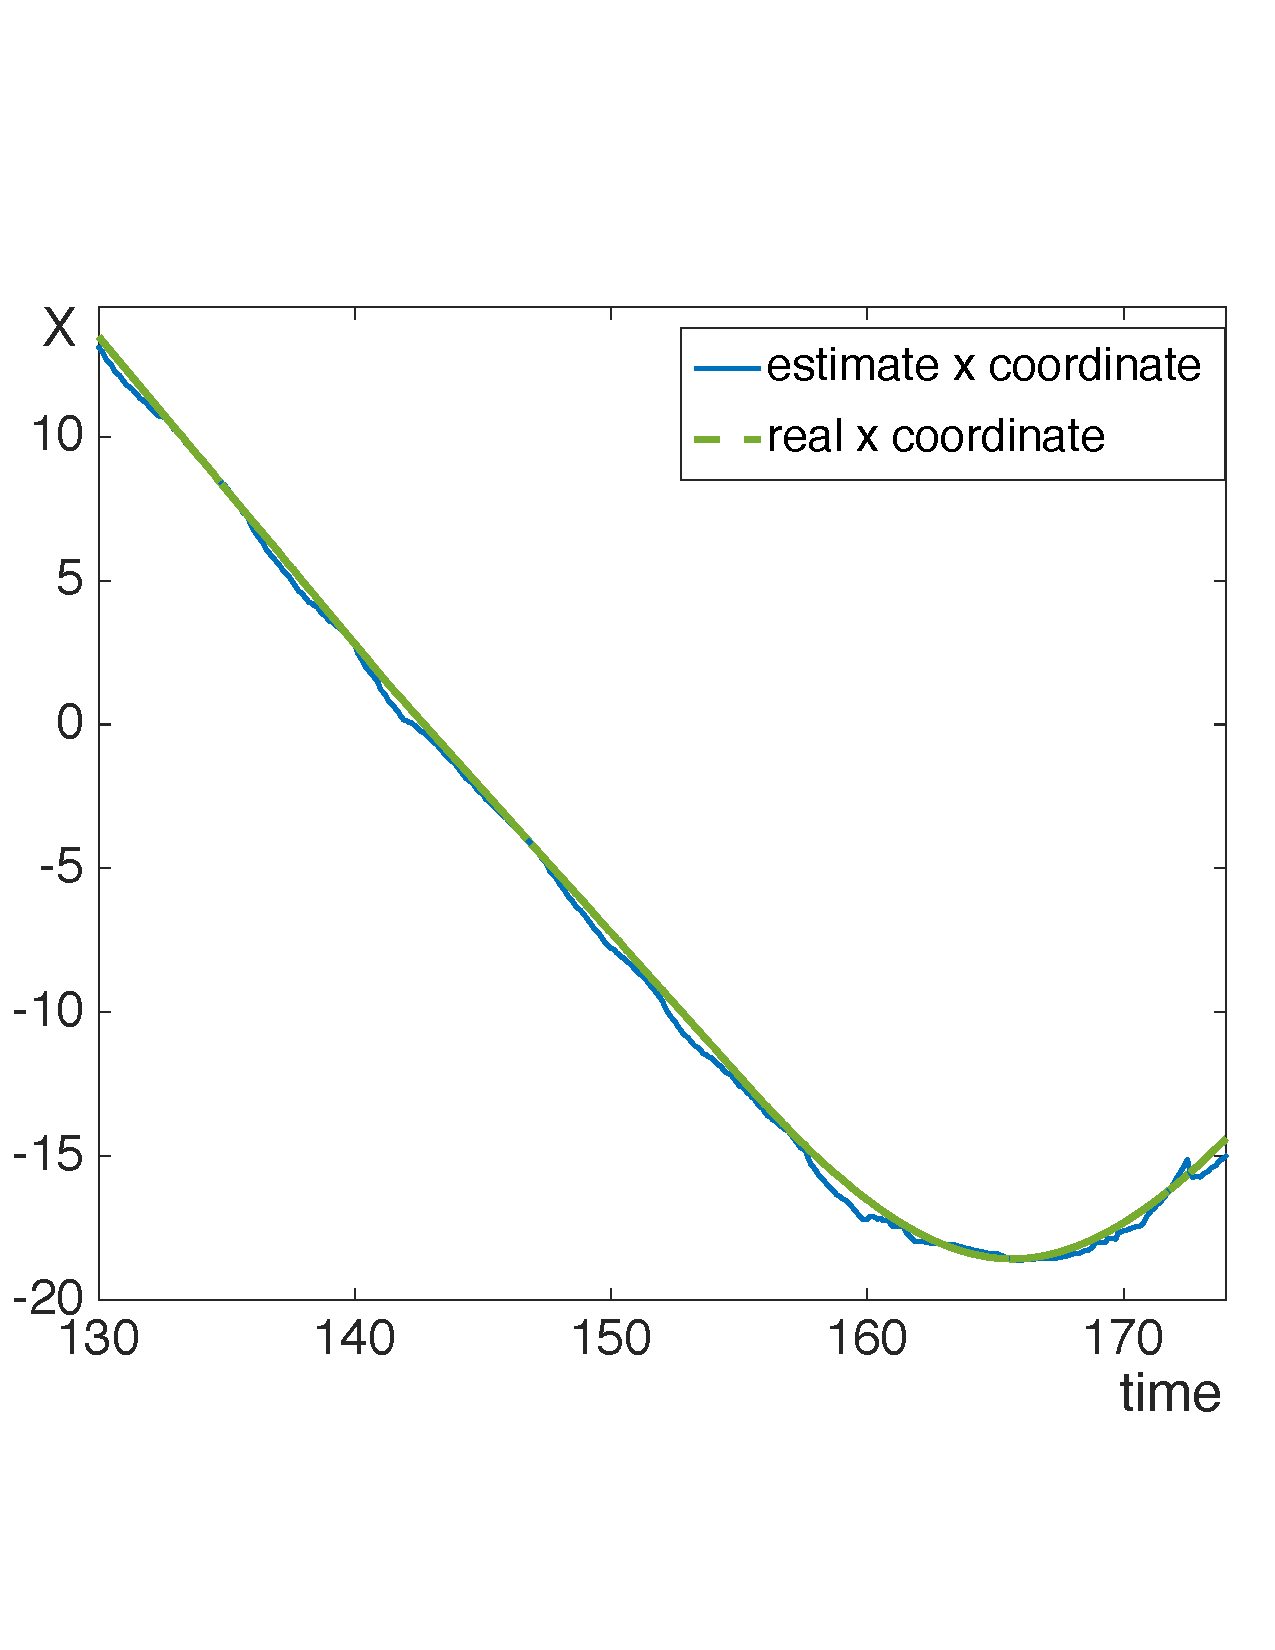
\includegraphics[width=\textwidth]{img/high_altitude_error_x.pdf}
        \caption{x }
        \label{fig:one}
   \end{subfigure}
   \begin{subfigure}[b]{0.4\textwidth}
        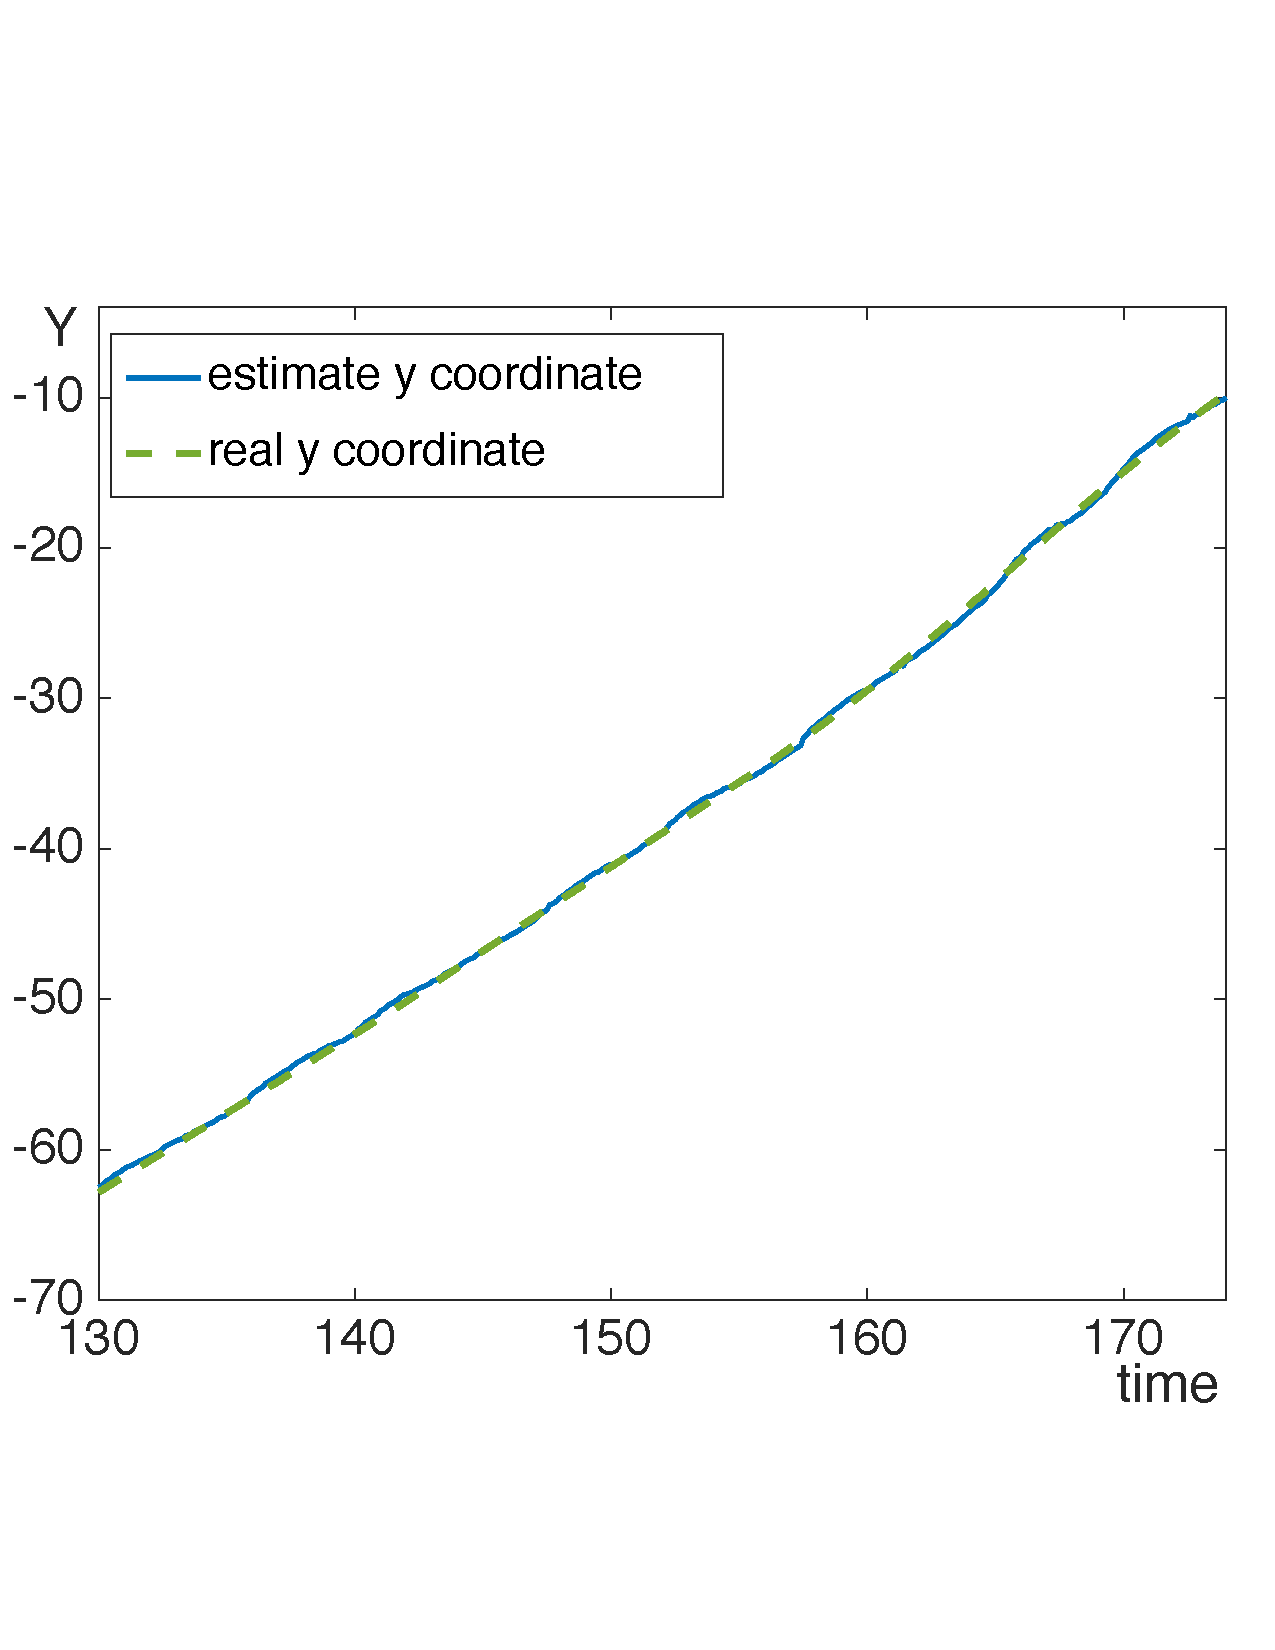
\includegraphics[width=\textwidth]{img/high_altitude_error_y.pdf}
        \caption{y}
        \label{fig:two}
   \end{subfigure}
  \caption{Comparison between estimate position (blue dots) and real position (green line) in simulation. The platform is moving in the 8 shape path at 1.5m/s and the quadrotor explores the area at 15m of altitude.}
  \label{fig:ekf_high_altitude_comparison}
\end{figure} 

As one can see from the graph \ref{fig:ekf_high_altitude_error}, the estimation error can be really high during this phase. In particular the chart shows the average error between $x$ and $y$ directions and the correspondent RMSE from a searching at 15m of altitude.\\
This data even if are not really precise are good enough to perform the first stage two and three of the state machine.
\begin{figure}[!ht]
    \centering
    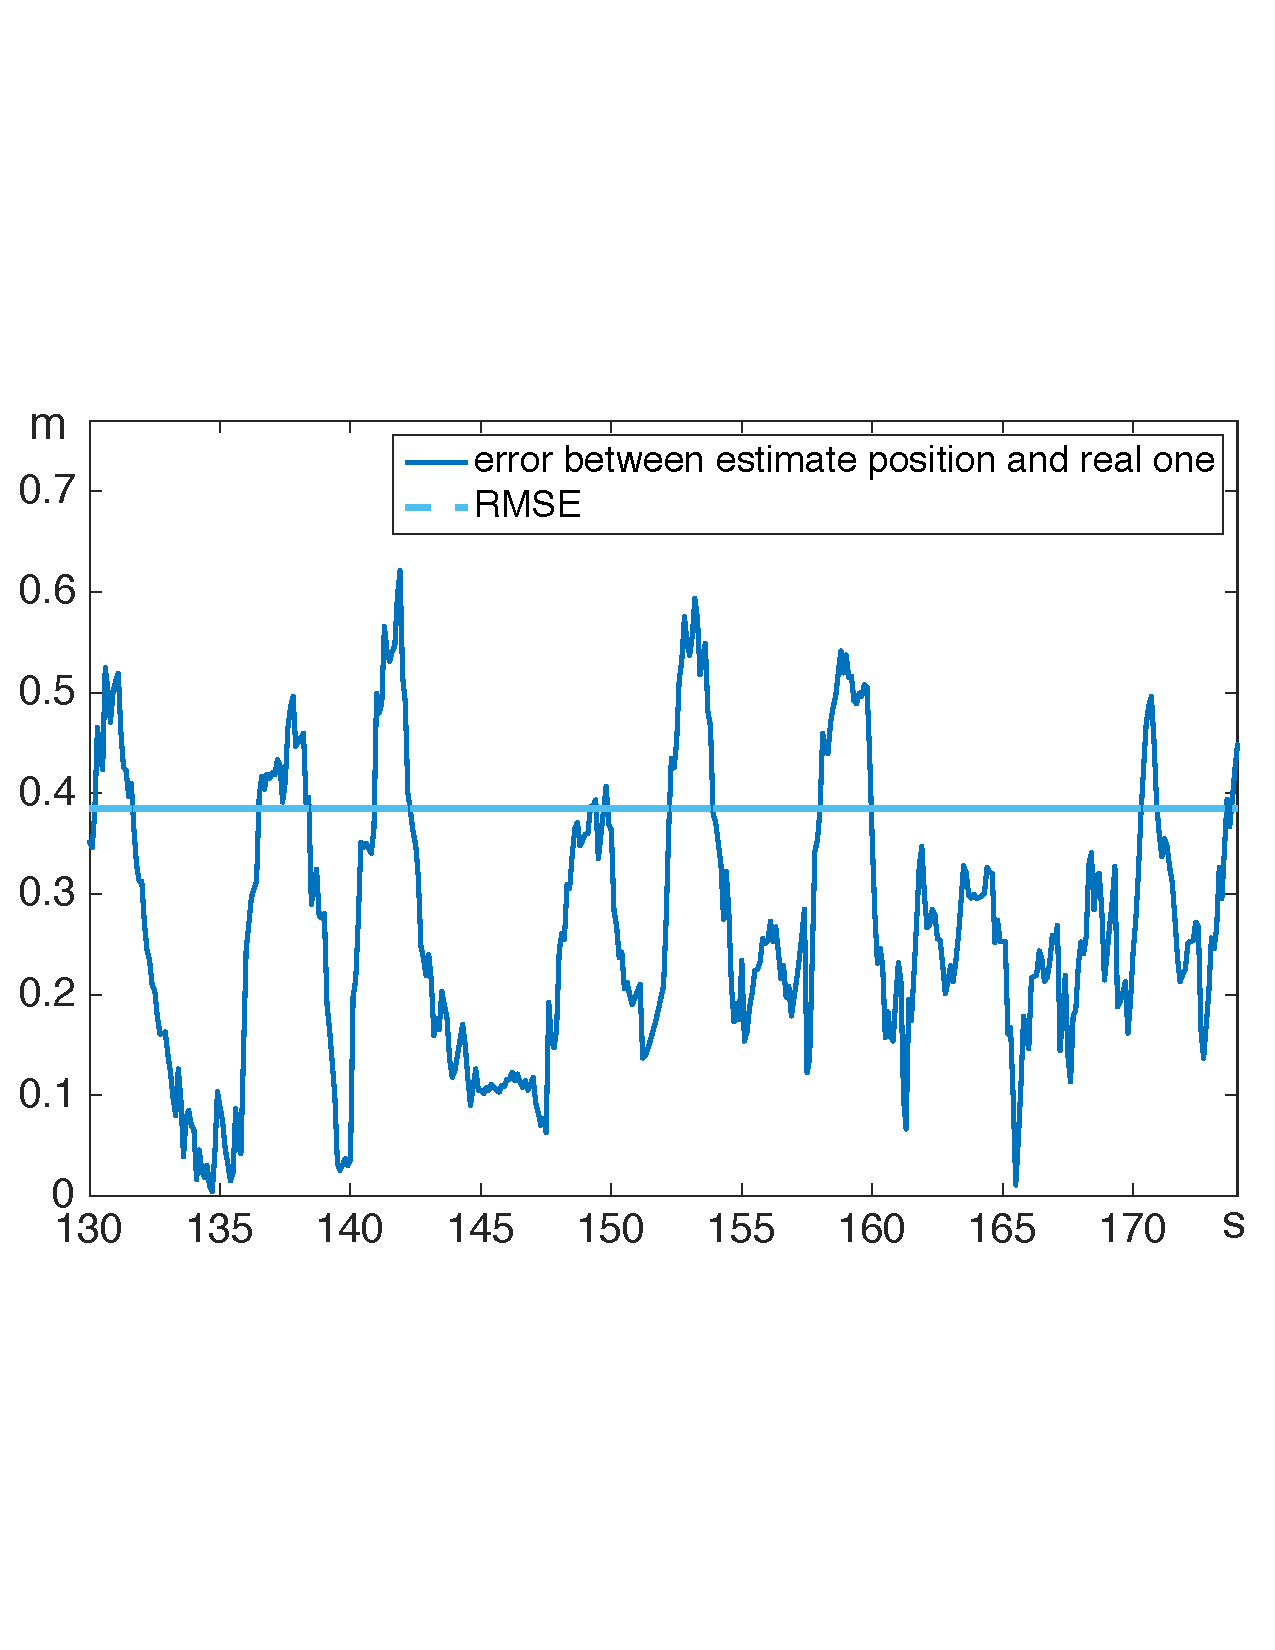
\includegraphics[width=0.7\textwidth]{img/high_altitude_error.pdf}
      \caption{Average error between estimate and real x,y coordinate. The RMSE is below 40cm. The value seems high but the estimation is taken from 15m high and while both quadrotor and platform are moving. This precision is sufficient to estimate the type of movement of the base.}
    \label{fig:ekf_high_altitude_error}
\end{figure}

TODO images from real world moving platform HIGH ALTITUDE
\begin{figure}[!ht]
    \centering
    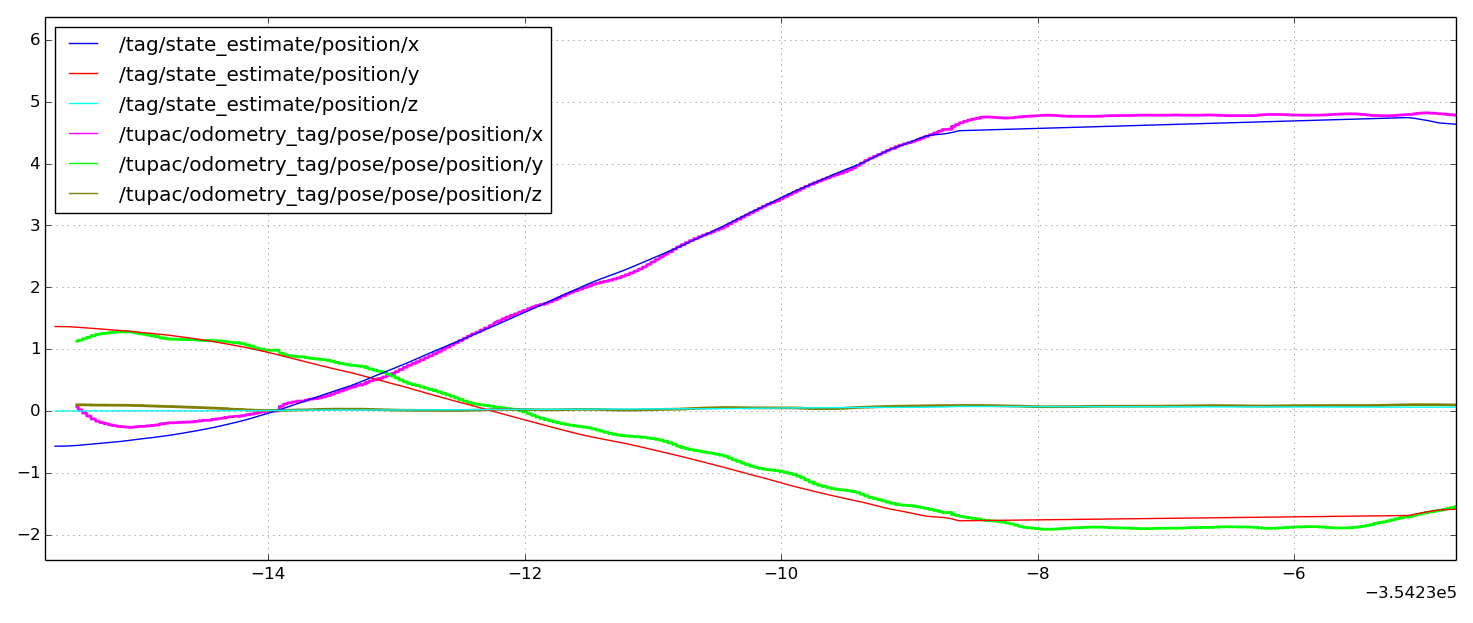
\includegraphics[width=0.7\textwidth]{img/position_real_world.png}
    \caption{Real world test. Comparison between estimate position and ground truth for a platform moving at $1\frac{m}{s}$}
    \label{fig:ekf_position_real}
\end{figure}

\begin{figure}[!ht]
    \centering
    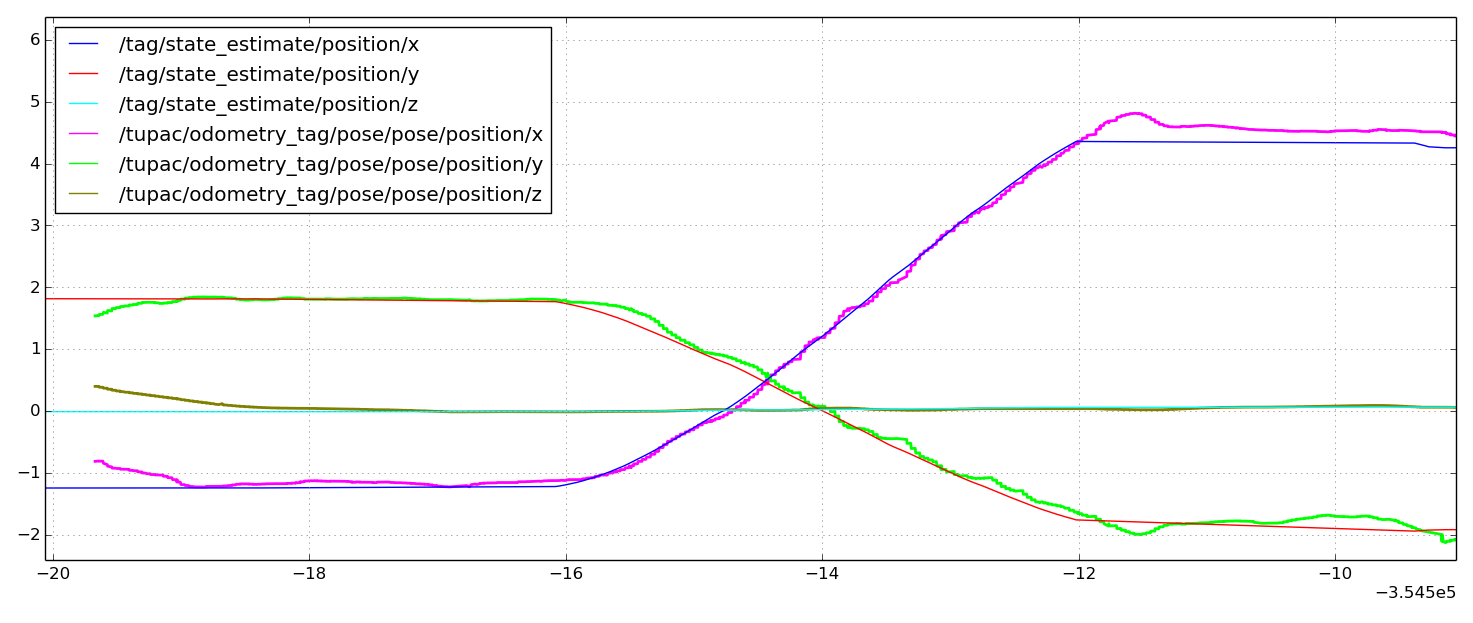
\includegraphics[width=0.7\textwidth]{img/position_real_world_fast.png}
      \caption{Real world test. Comparison between estimate position and ground truth for a platform moving at $2\frac{m}{s}$}
    \label{fig:ekf_position_real_fast}
\end{figure}


\newpage

\subsection{From low altitude}
\subsubsection{Different AR-Tag detector}
In the real world implementation we tried several different tag detector ROS packages, such as  RPG-April-Tags \cite{rpgapriltags} that uses the  AprilTags library \cite{apriltagslibrary}, AR-Sys \cite{arsys} and AR-Track-Alvar \cite{artrackalvar}.\\
All of them have some strengths and weaknesses and we compared the most important features to understand which detector is the more suitable for our purpose:
\begin{itemize}
\item \textbf{Light conditions}: all these methods uses the edge based approach, so the results is similar in different light conditions.
\item \textbf{Final pose}: all trackers solve a PnP Problem to find the 6dof pose of the camera that minimize the reprojection error of the points on the image. The final result is the transformation between tag and camera. RPG-AprilTag has also the possibility to return a 4dof pose (perfect for our application), saving some computation.
\item \textbf{Multiple tags}: AR-Sys and AR-Track-Alvar possess the ability to directly track multiple tags or single target composed by multiple tags.
\item \textbf{Precision}: we measure the error at $1m$ distance from the tag
\begin{itemize}
\item RPG-April-Tags: $\pm 1 pixel $ 
\item AR-Sys: $\pm 2 pixel $
\item AR-Track-Alvar: $\pm 1 pixel $
\end{itemize}
\item \textbf{Frequency}: on the quadrotor the performance of the three tracker where quite different
\begin{itemize}
\item RPG-April-Tags: $~1Hz$
\item AR-Sys: $~4Hz$
\item AR-Track-Alvar: $~1Hz$
\end{itemize}
\end{itemize}

\paragraph{AR-Sys}
In our final implementation we decided to use AR-Sys because its computational efficiency. AR-Sys is 3D pose estimation ROS package that uses ARUco marker boards \cite{Aruco2014}.\\
This package guarantees a good error correction in the identification of a specific tag, and, more interesting for our application, a solution to the occlusion problem using multiple markers.\\
It can identify the pose of boards composed by multiple tags considered as a single unit. The board is defined in an XML file where all the tag are listed with an ID and the relative position w.r.t. the master tag (the first in the list) that defines the center of the cumulative target, the pose of the camera is given with respect to this tag. This feature guarantees more stable pose estimates and robustness to the occlusion of a part of the platform.

\subsubsection{Results}
Very accurate pose estimation is obtain when the AR tags are used. Generally the error in the $x,y$ coordinate is less then $10cm$ while in the $z$ direction is about $3cm$.\\

The following figures show different experiments in the real world and in the simulation with different velocities and initial values.\\

\begin{figure}[!htbp]
  \centering
   \begin{subfigure}[b]{0.45\textwidth}
        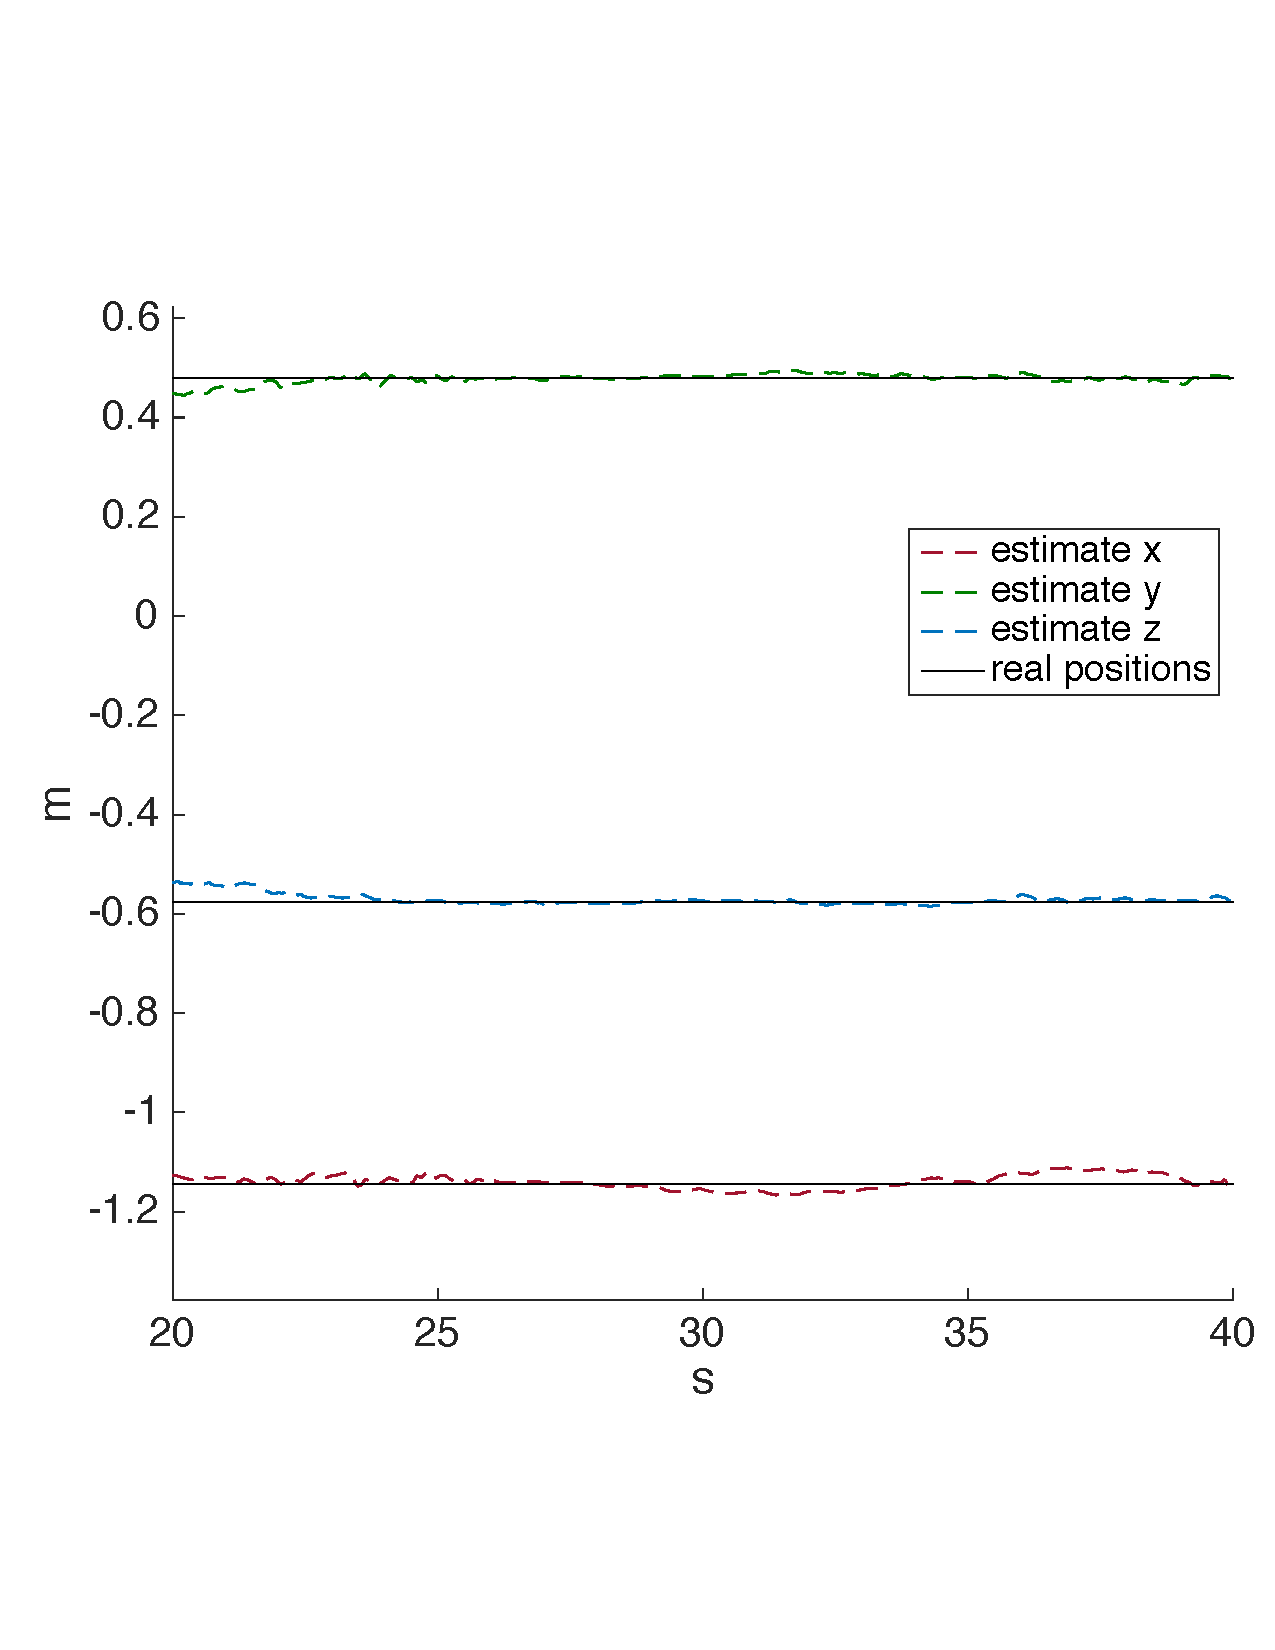
\includegraphics[width=\textwidth]{img/tag_static_real_world_pos.pdf}
        \caption{Position }
        \label{fig:one_ekf_real_world_static}
   \end{subfigure}\hfill
   \begin{subfigure}[b]{0.45\textwidth}
        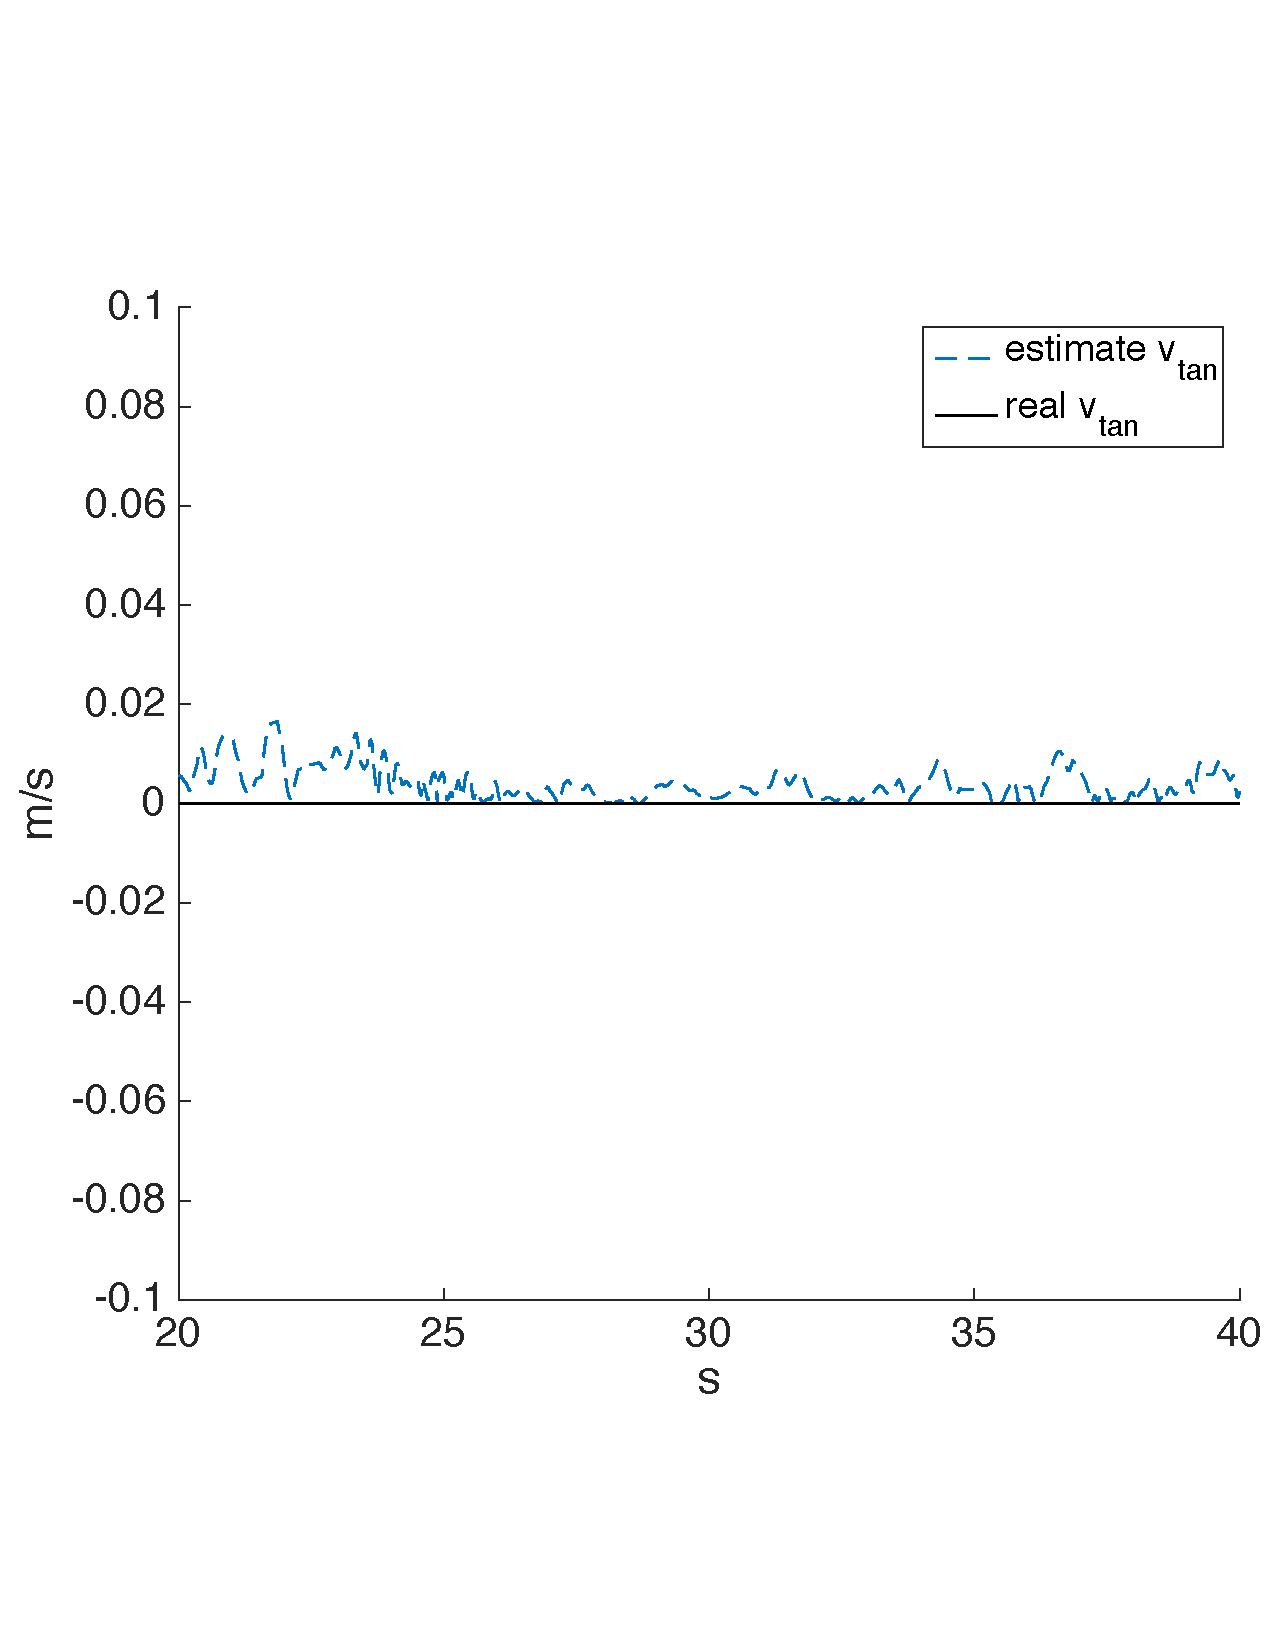
\includegraphics[width=\textwidth]{img/tag_static_real_world_vel.pdf}
        \caption{Velocity}
        \label{fig:two_ekf_real_world_static}
   \end{subfigure}
  \caption{Real world experiment. Comparison between estimate position and velocity with the ground truth values for a static platform. The estimate position has a RMSE of $5cm$ in $x,y$ and $2.5cm$ in $z$.}
  \label{fig:ekf_real_world_static}
\end{figure} 

\begin{figure}[!htbp]
  \centering
   \begin{subfigure}[b]{0.45\textwidth}
        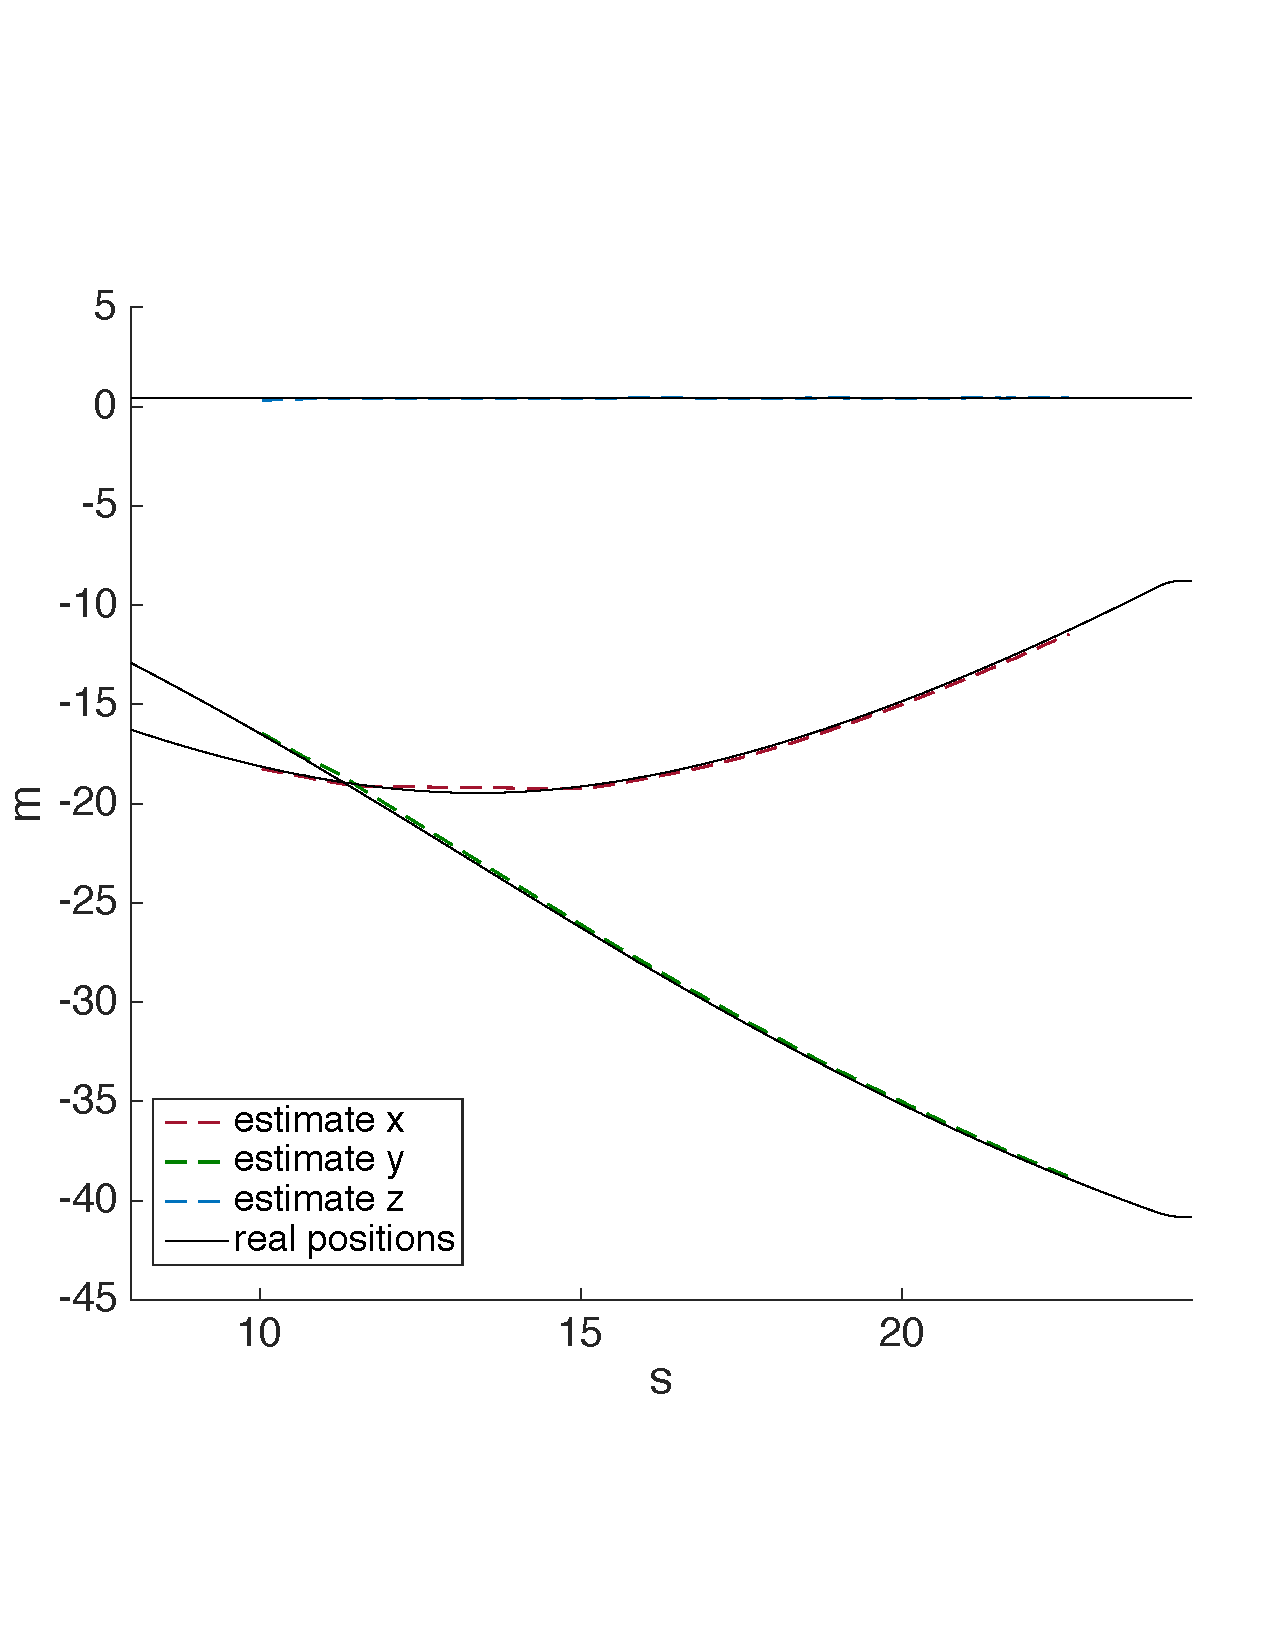
\includegraphics[width=\textwidth]{img/tag_2ms_simulation_pos.pdf}
        \caption{Position }
        \label{fig:one_ekf_simulation_2ms}
   \end{subfigure}\hfill
   \begin{subfigure}[b]{0.45\textwidth}
        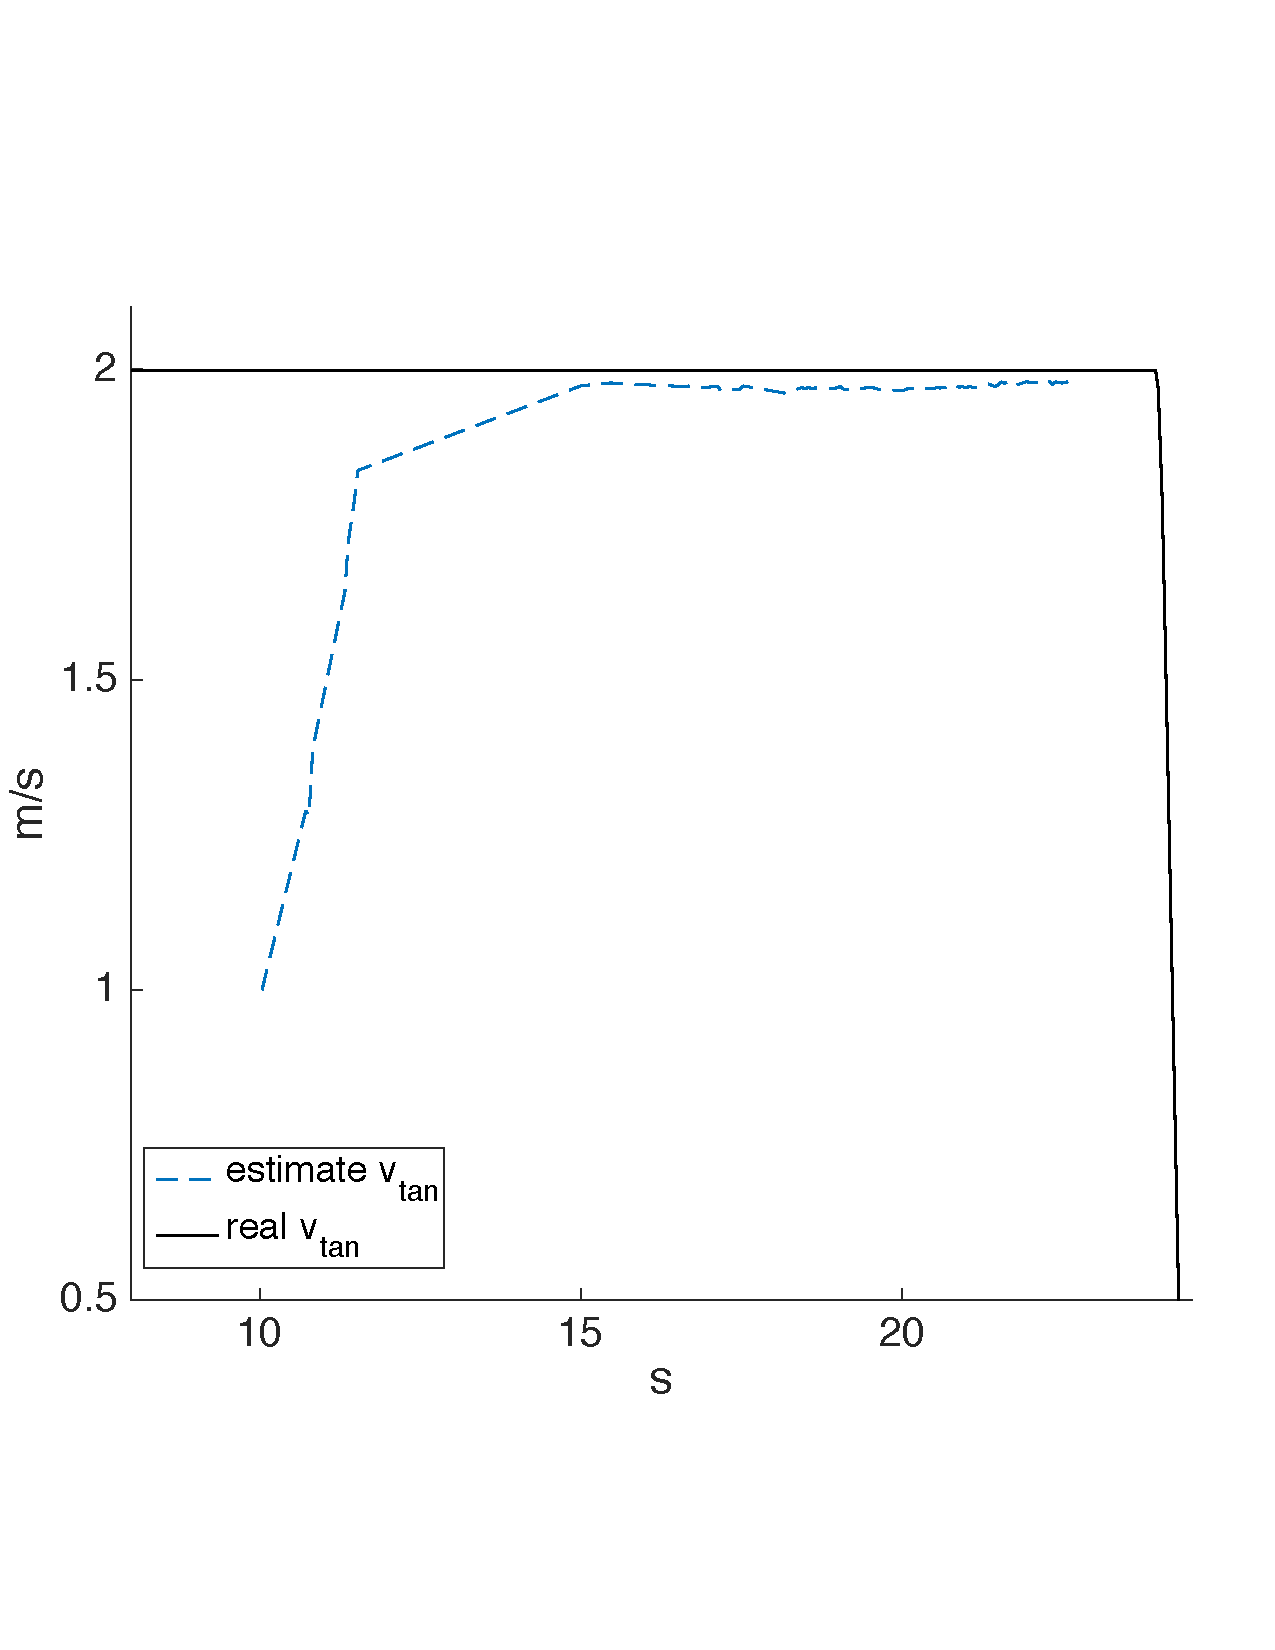
\includegraphics[width=\textwidth]{img/tag_2ms_simulation_vel.pdf}
        \caption{Velocity}
        \label{fig:two_ekf_simulation_2ms}
   \end{subfigure}
  \caption{Simulation test. Comparison between estimate position and velocity with the ground truth values. The velocity is initialized with a wrong value of 1m/s but the filter needs few steps to converge to the right value of 2m/s. The estimate position has a RMSE of $10cm$ in $x,y$ and $2cm$ in $z$.}
  \label{fig:ekf_simulation_2ms}
\end{figure} 


%\begin{figure}[!htbp]
%  \centering
%   \begin{subfigure}[b]{0.45\textwidth}
%        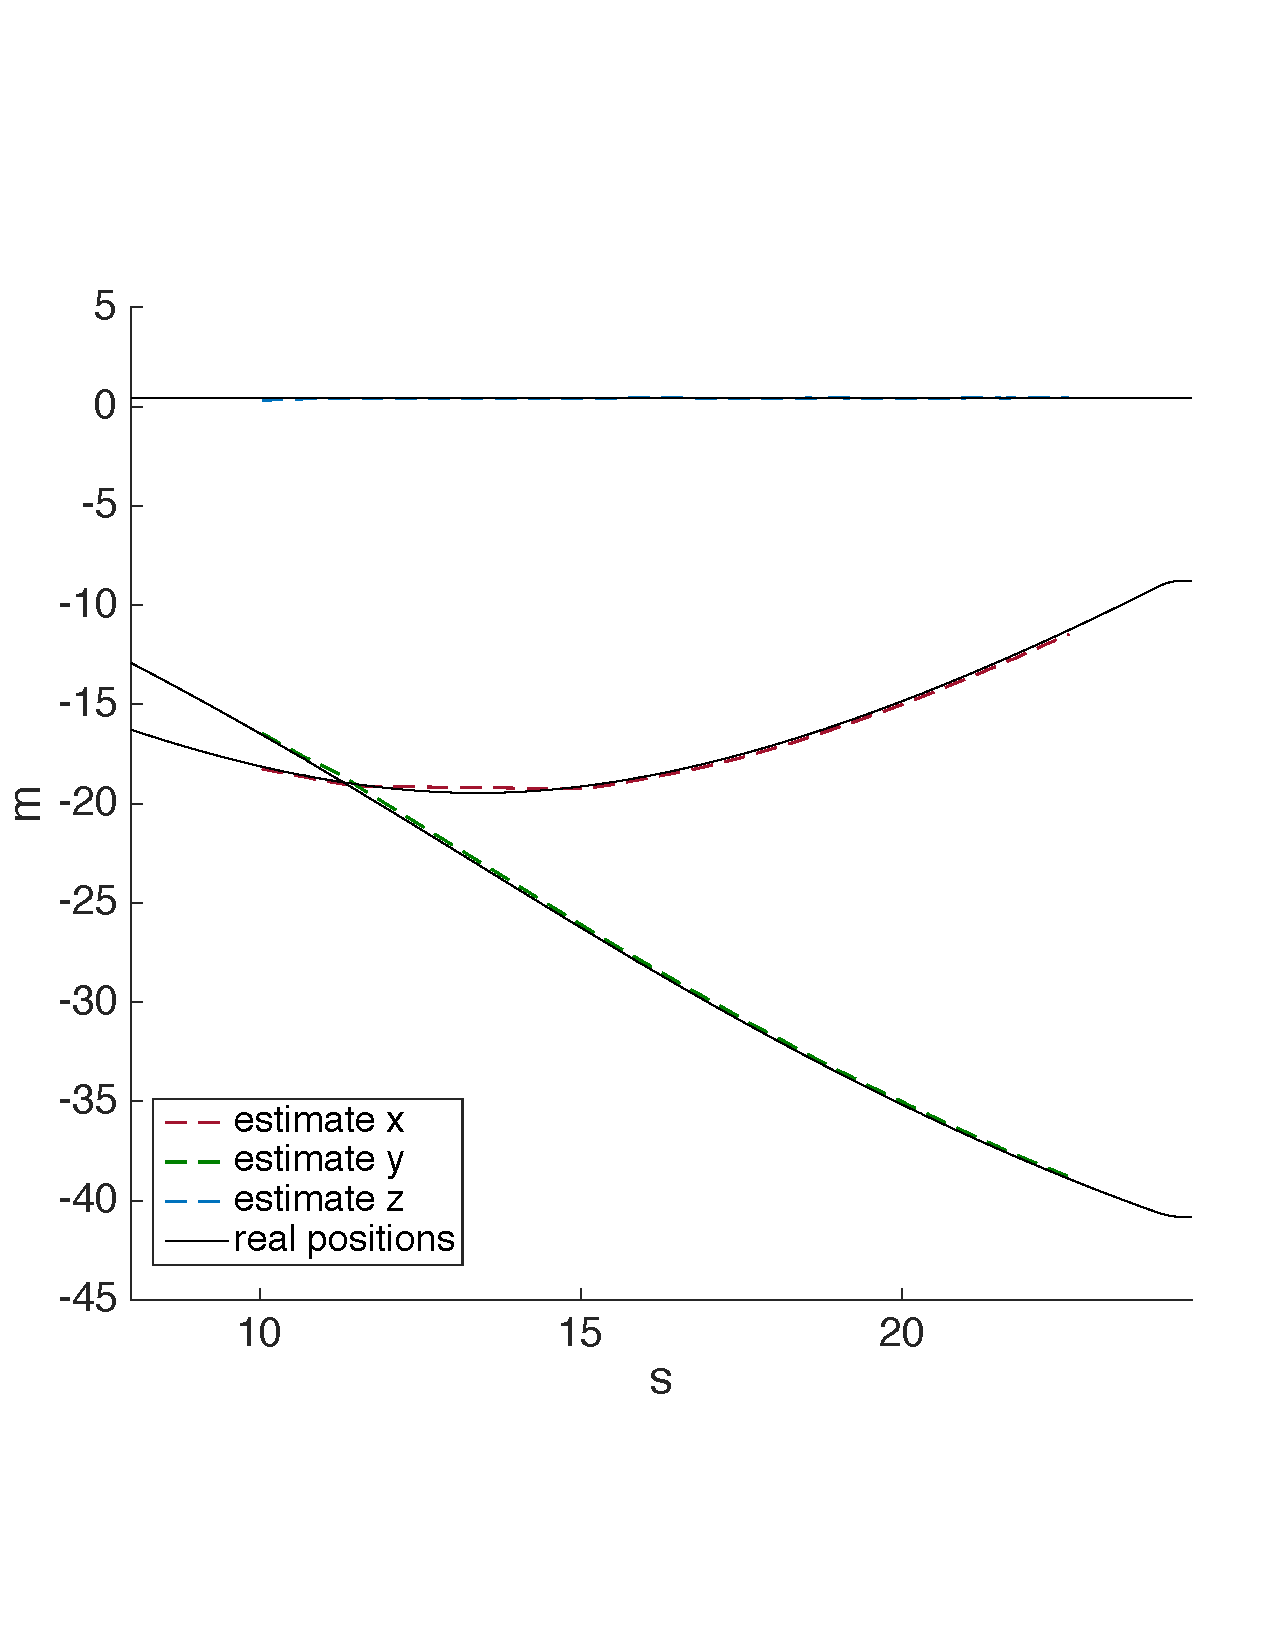
\includegraphics[width=\textwidth]{img/tag_2ms_simulation_pos.pdf}
%        \caption{Position }
%        \label{fig:one}
%   \end{subfigure}\hfill
%   \begin{subfigure}[b]{0.45\textwidth}
%        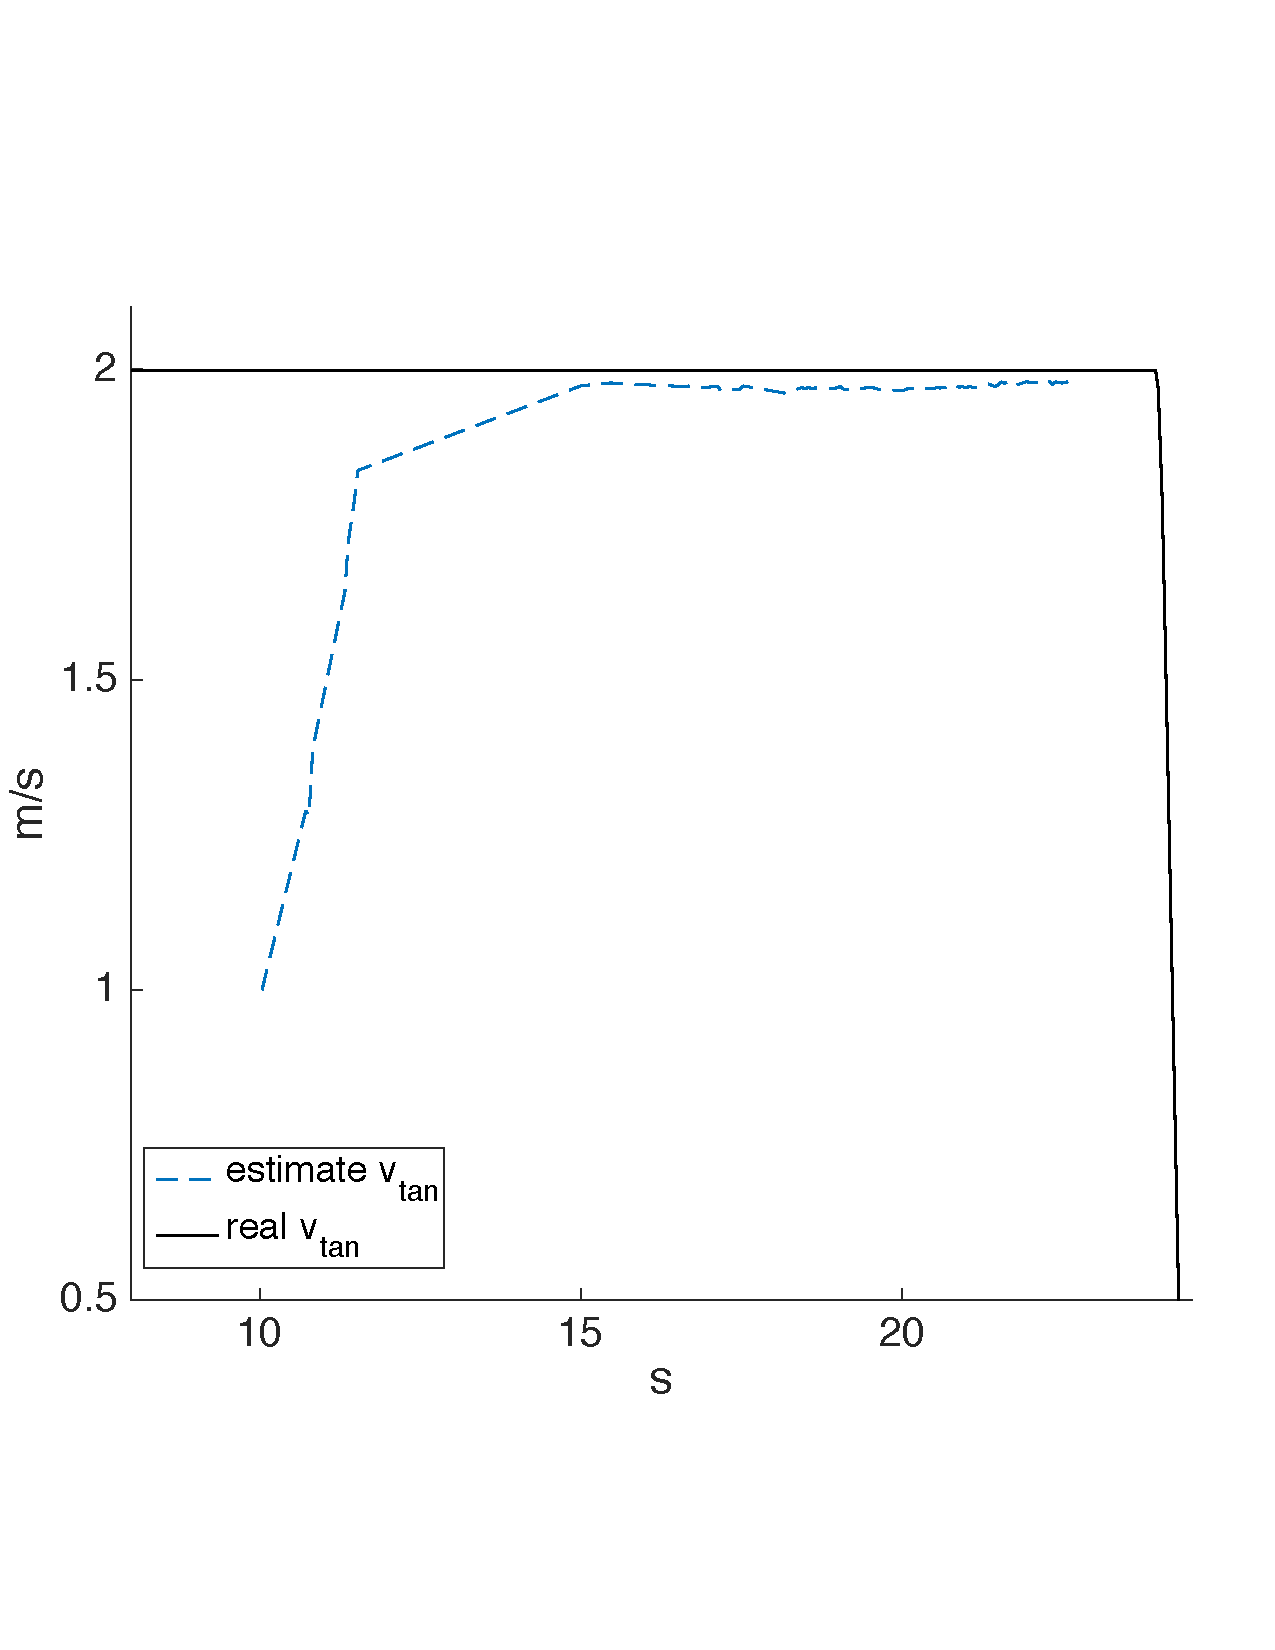
\includegraphics[width=\textwidth]{img/tag_2ms_simulation_vel.pdf}
%        \caption{Velocity}
%        \label{fig:two}
%   \end{subfigure}
%  \caption{Simulation test. Comparison between estimate position and velocity with the ground truth values. The velocity is initialized with 0 value. In this case the filter needs some time to converge to the right value of velocity.}
%  \label{fig:ekf_simulation_hot_init}
%\end{figure}

TODO images from real world moving platform
\begin{figure}[!ht]
    \centering
    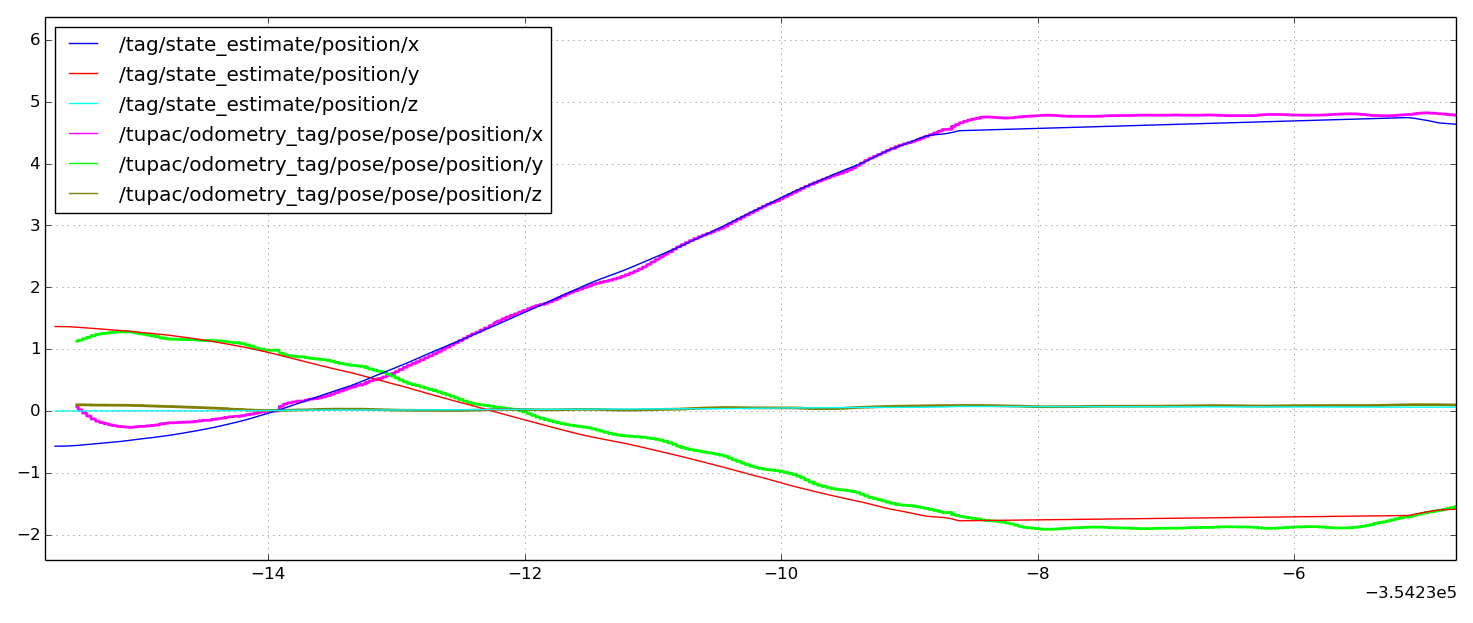
\includegraphics[width=0.8\textwidth]{img/position_real_world.png}
    \caption{Real world test. Comparison between estimate position and ground truth for a platform moving at $1\frac{m}{s}$}
    \label{fig:ekf_position_real}
\end{figure}

\begin{figure}[!ht]
    \centering
    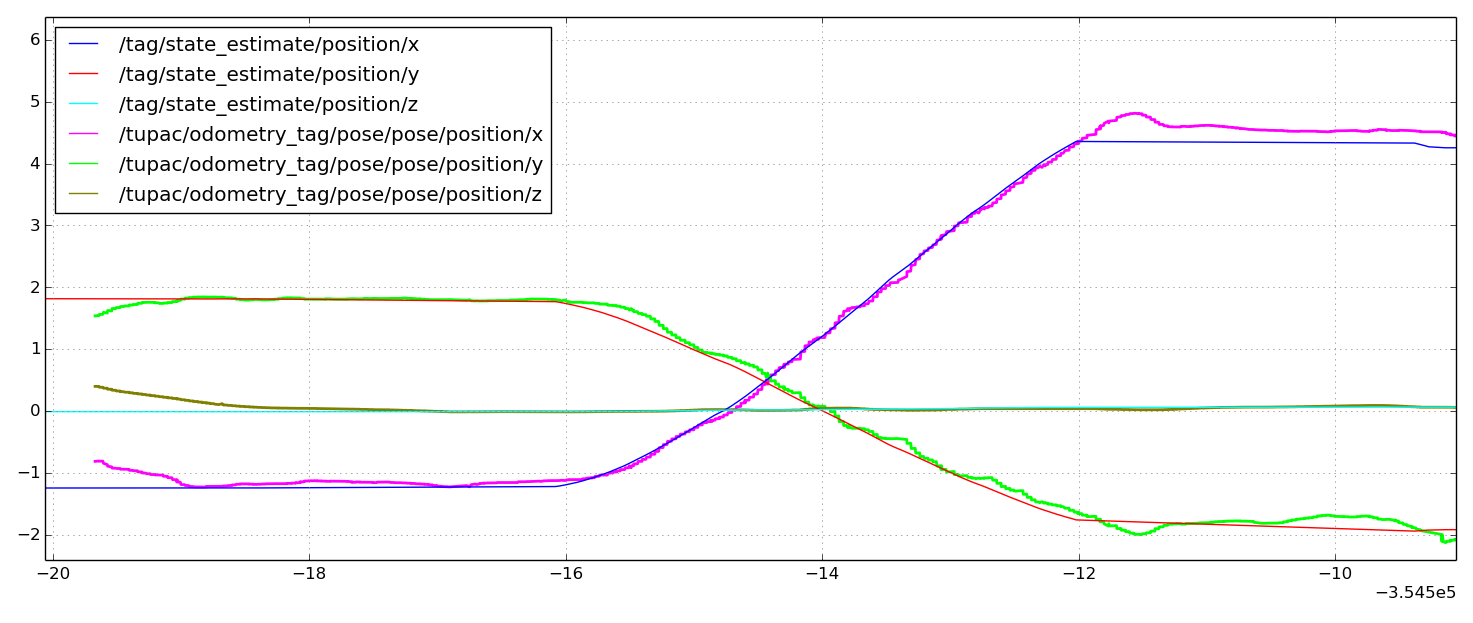
\includegraphics[width=0.8\textwidth]{img/position_real_world_fast.png}
      \caption{Real world test. Comparison between estimate position and ground truth for a platform moving at $2\frac{m}{s}$}
    \label{fig:ekf_position_real_fast}
\end{figure}

\newpage

\section{Trajectory generation}

\subsection{Acceleration estimation} \label{subsec:acceleration_experiments}
We described in \ref{subsec:acceleration} the three possible methods to estimate the acceleration of the quadrotor at a given time. This calculation is necessary because the trajectory generator needs a full state description of the initial condition of the quadtotor [position,velocity,acceleration] in order to solve the optimal control problem.\\
We took several data sets while the quadrotor was flying in the flyingroom in order to compare the different methods used to approximate the accelerations.\\

To understand how the raw data looks like, the figure \ref{fig:comparison_acc} on the first column compares the data taken directly from the IMU, with finite difference calculate with two subsequent velocity estimations (without filtering) and the estimation computed with the total thrust. While on the right column there is the same comparison, but this time we consider the filtered versions of the accelerations calculated with finite difference and with the data from the IMU.
\begin{figure}[!htbp]
 \centering   
     \begin{subfigure}[b]{0.45\textwidth}
     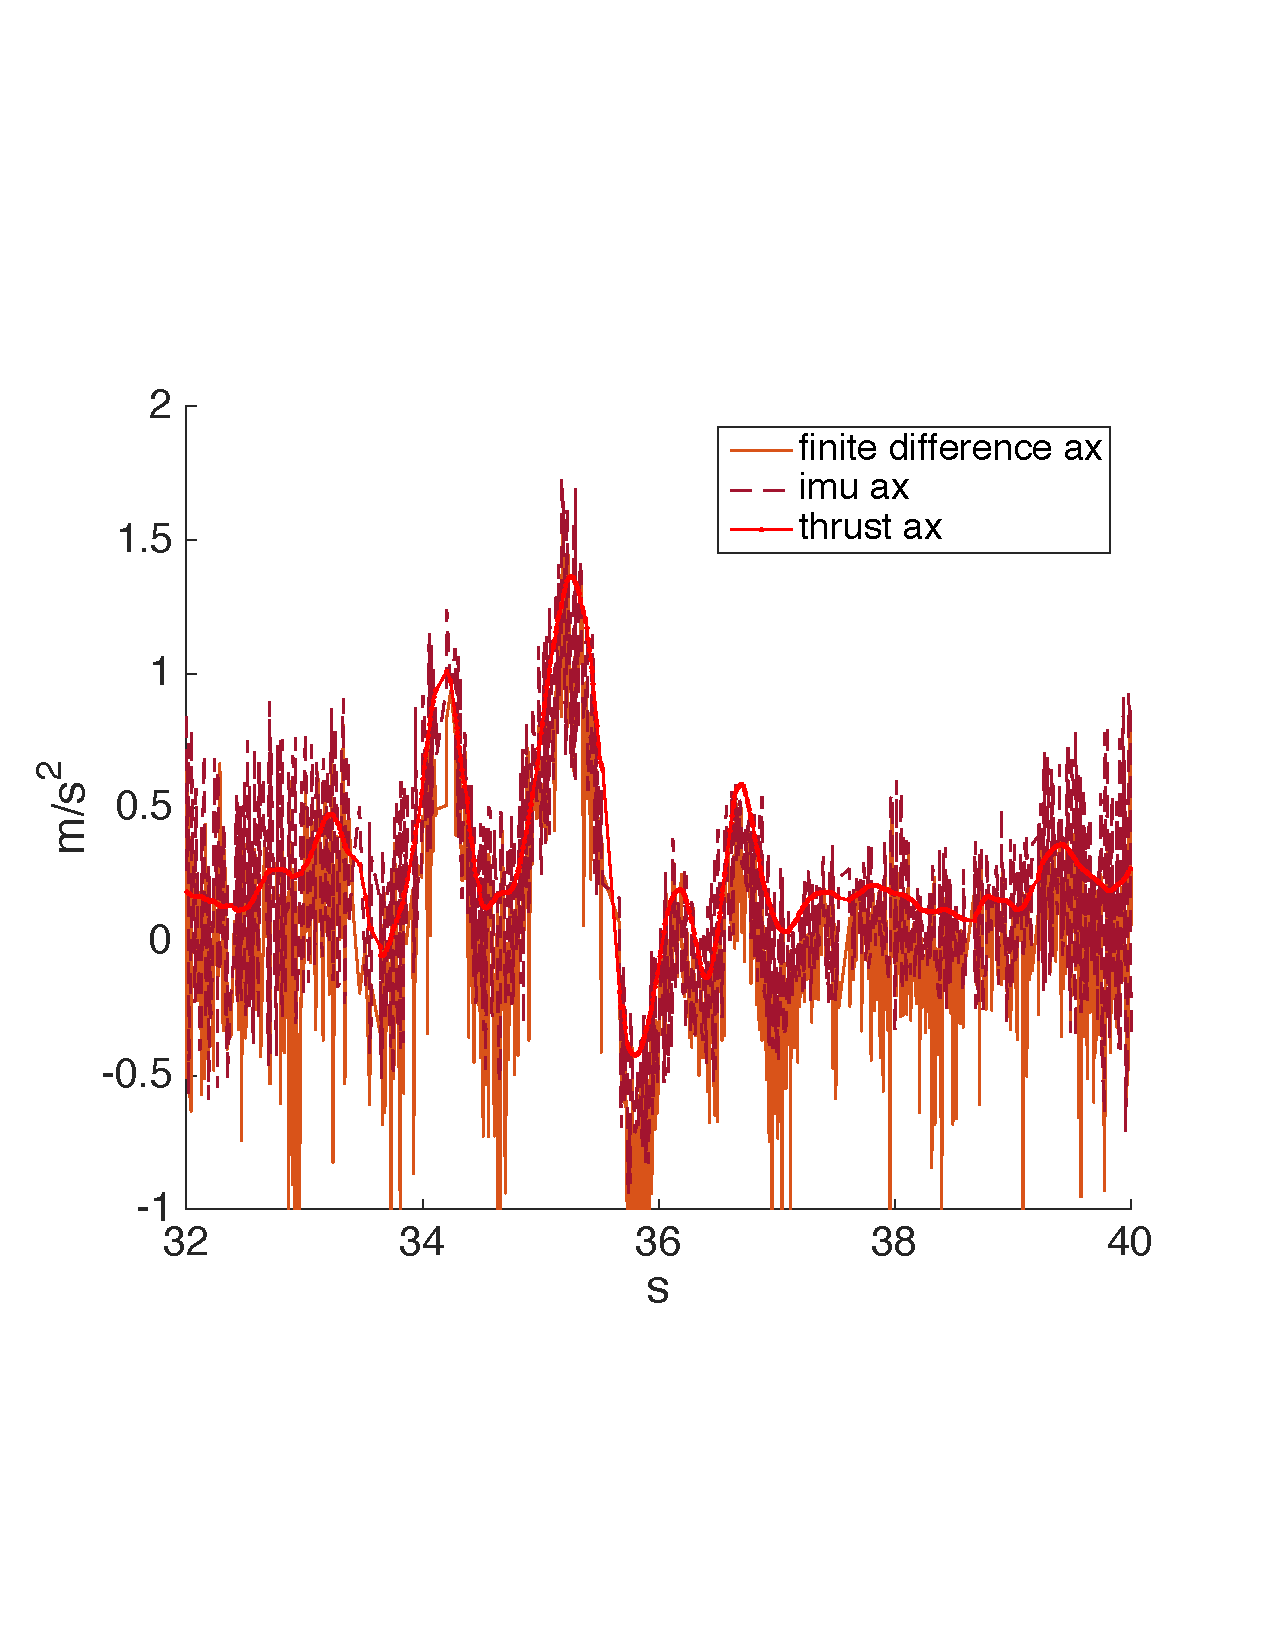
\includegraphics[width=\textwidth]{img/acceleration_mass_changed_no_filter_x.pdf}
        \caption{Acceleration x axis not filtered}
        \label{fig:comparison_accx}
   \end{subfigure}
    \begin{subfigure}[b]{0.45\textwidth}
     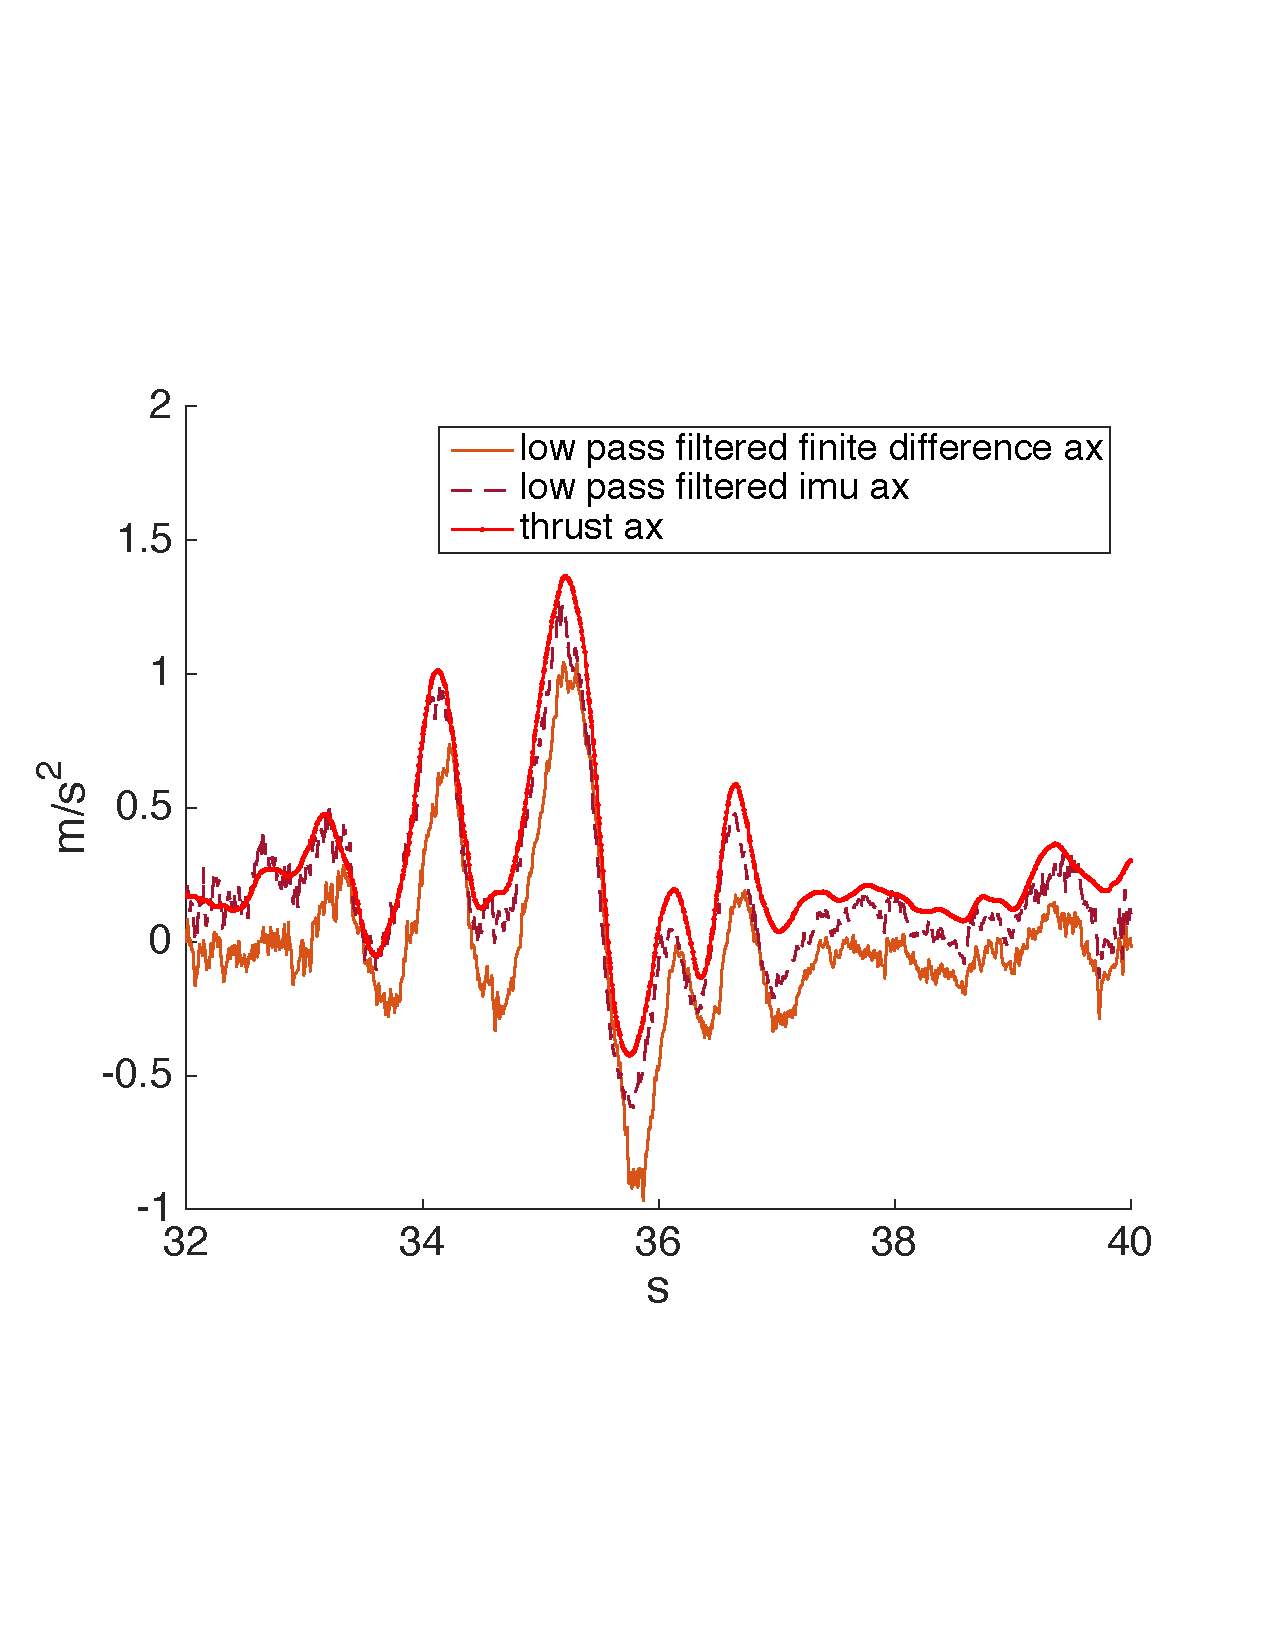
\includegraphics[width=\textwidth]{img/acceleration_mass_changed_filtered_x.pdf}
        \caption{Acceleration x axis filtered}
        \label{fig:comparison_accx_fil}
   \end{subfigure}\\[20pt]
   
   \begin{subfigure}[b]{0.45\textwidth}
     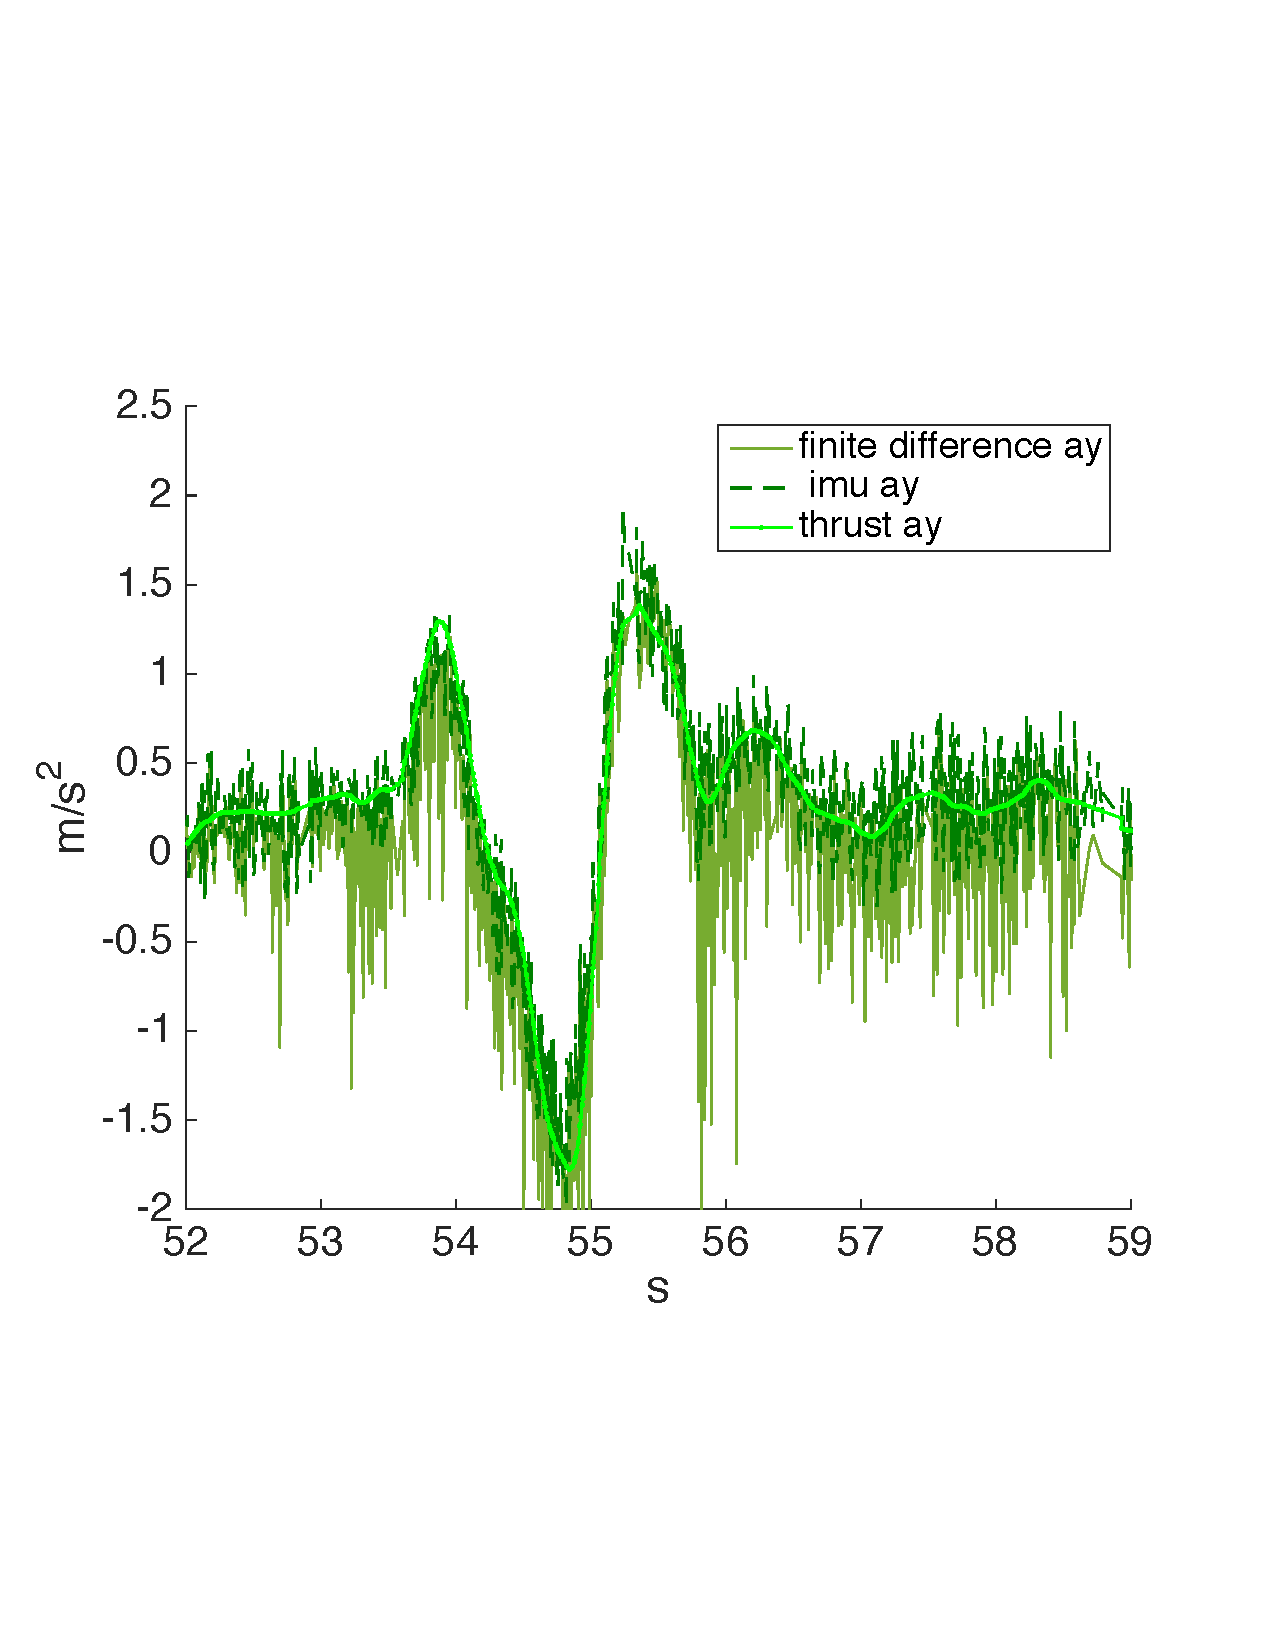
\includegraphics[width=\textwidth]{img/acceleration_mass_changed_no_filter_y.pdf}
        \caption{Acceleration y axis  not filtered}
        \label{fig:comparison_accy}
   \end{subfigure}
    \begin{subfigure}[b]{0.45\textwidth}
     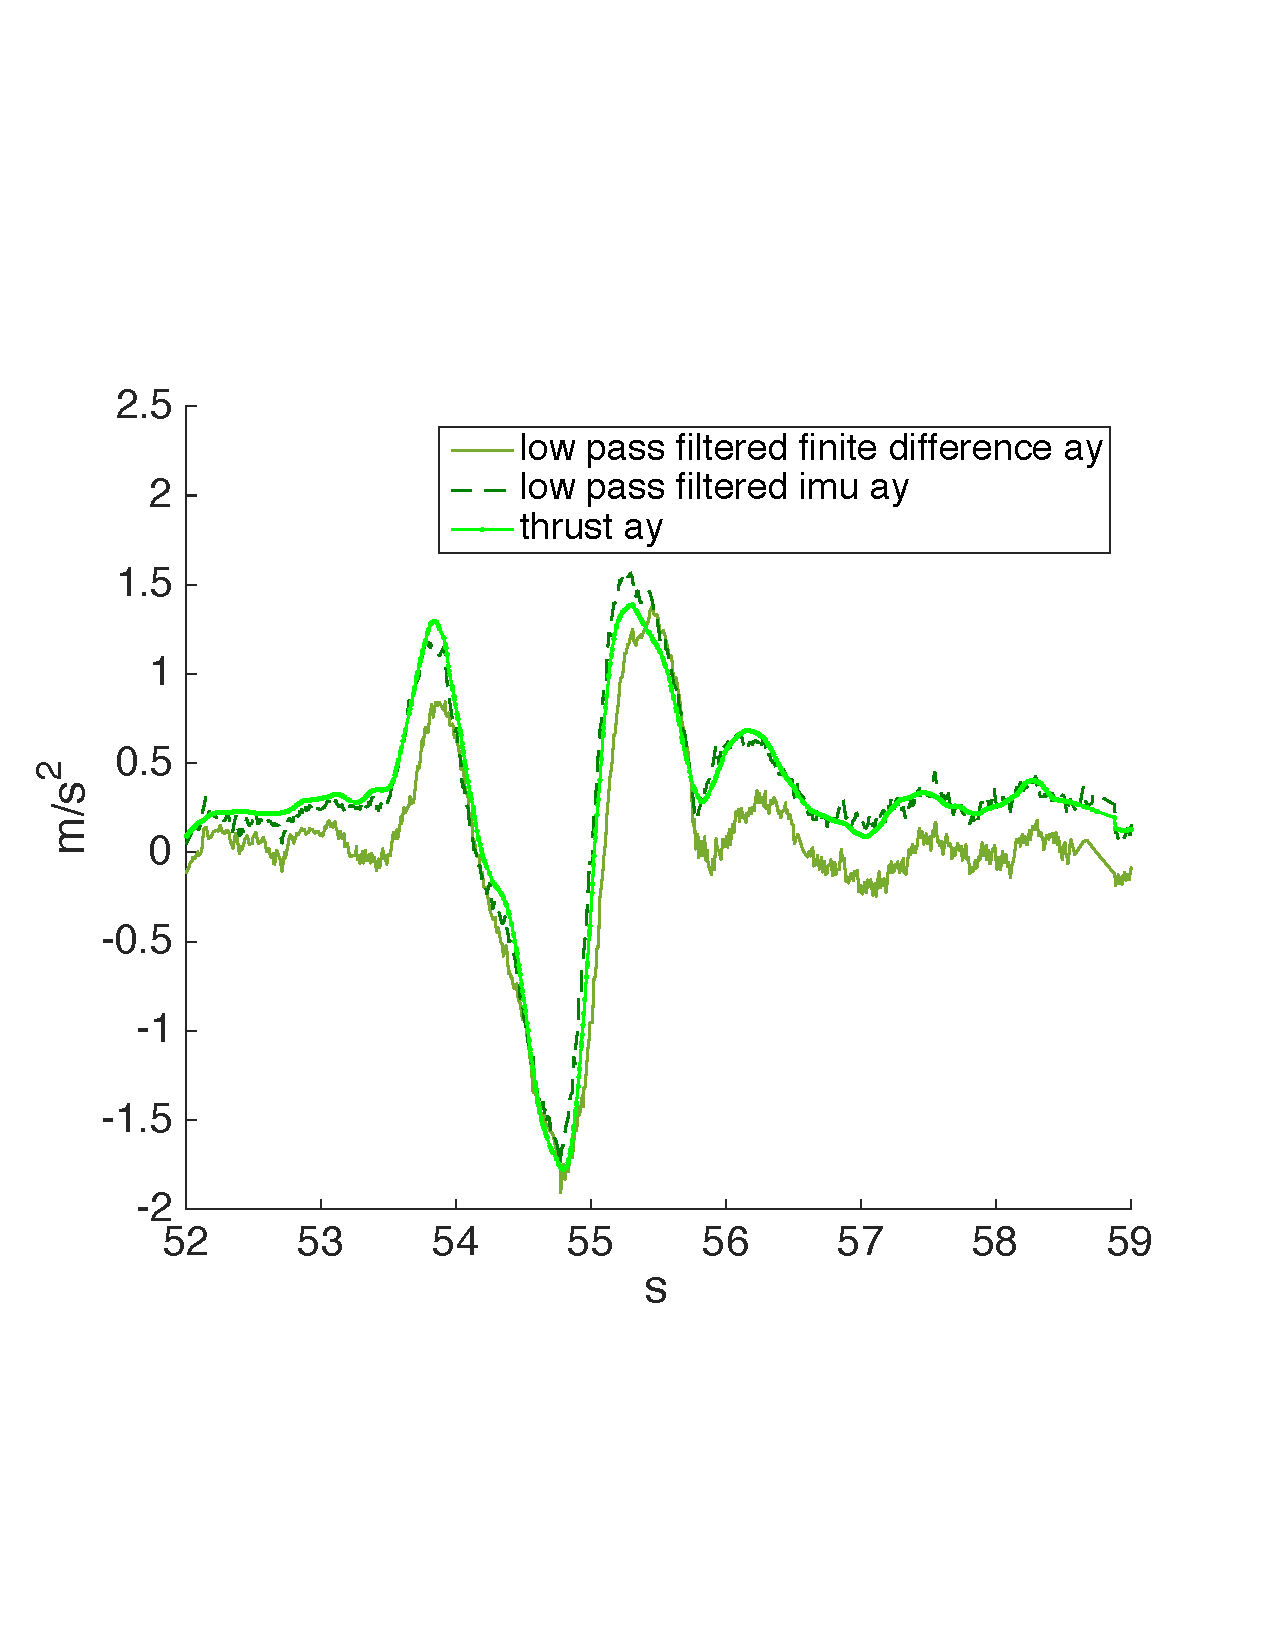
\includegraphics[width=\textwidth]{img/acceleration_mass_changed_filtered_y.pdf}
        \caption{Acceleration y axis filtered}
        \label{fig:comparison_accy_fil}
   \end{subfigure}\\[20pt]
   
    \begin{subfigure}[b]{0.45\textwidth}
     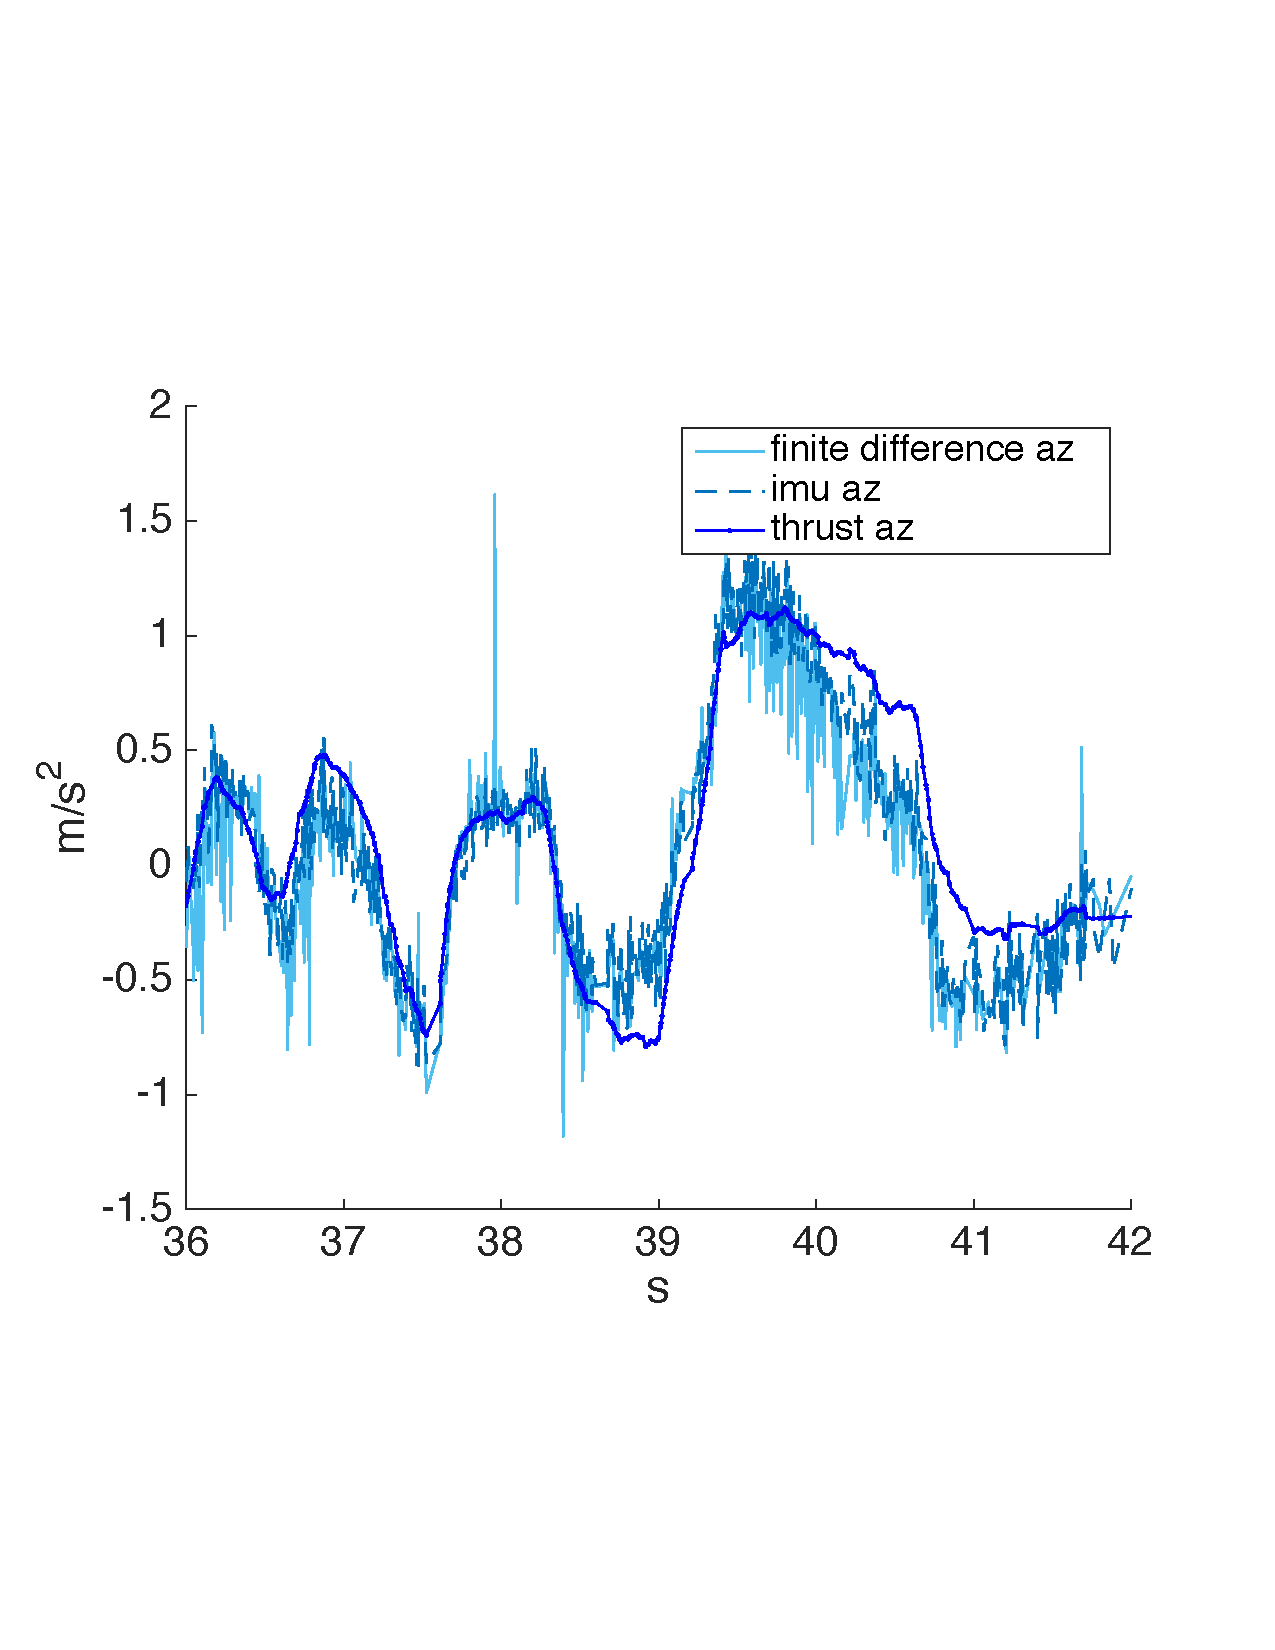
\includegraphics[width=\textwidth]{img/acceleration_mass_changed_no_filter_z.pdf}
        \caption{Acceleration z axis  not filtered}
        \label{fig:comparison_accz}
   \end{subfigure}
     \begin{subfigure}[b]{0.45\textwidth}
     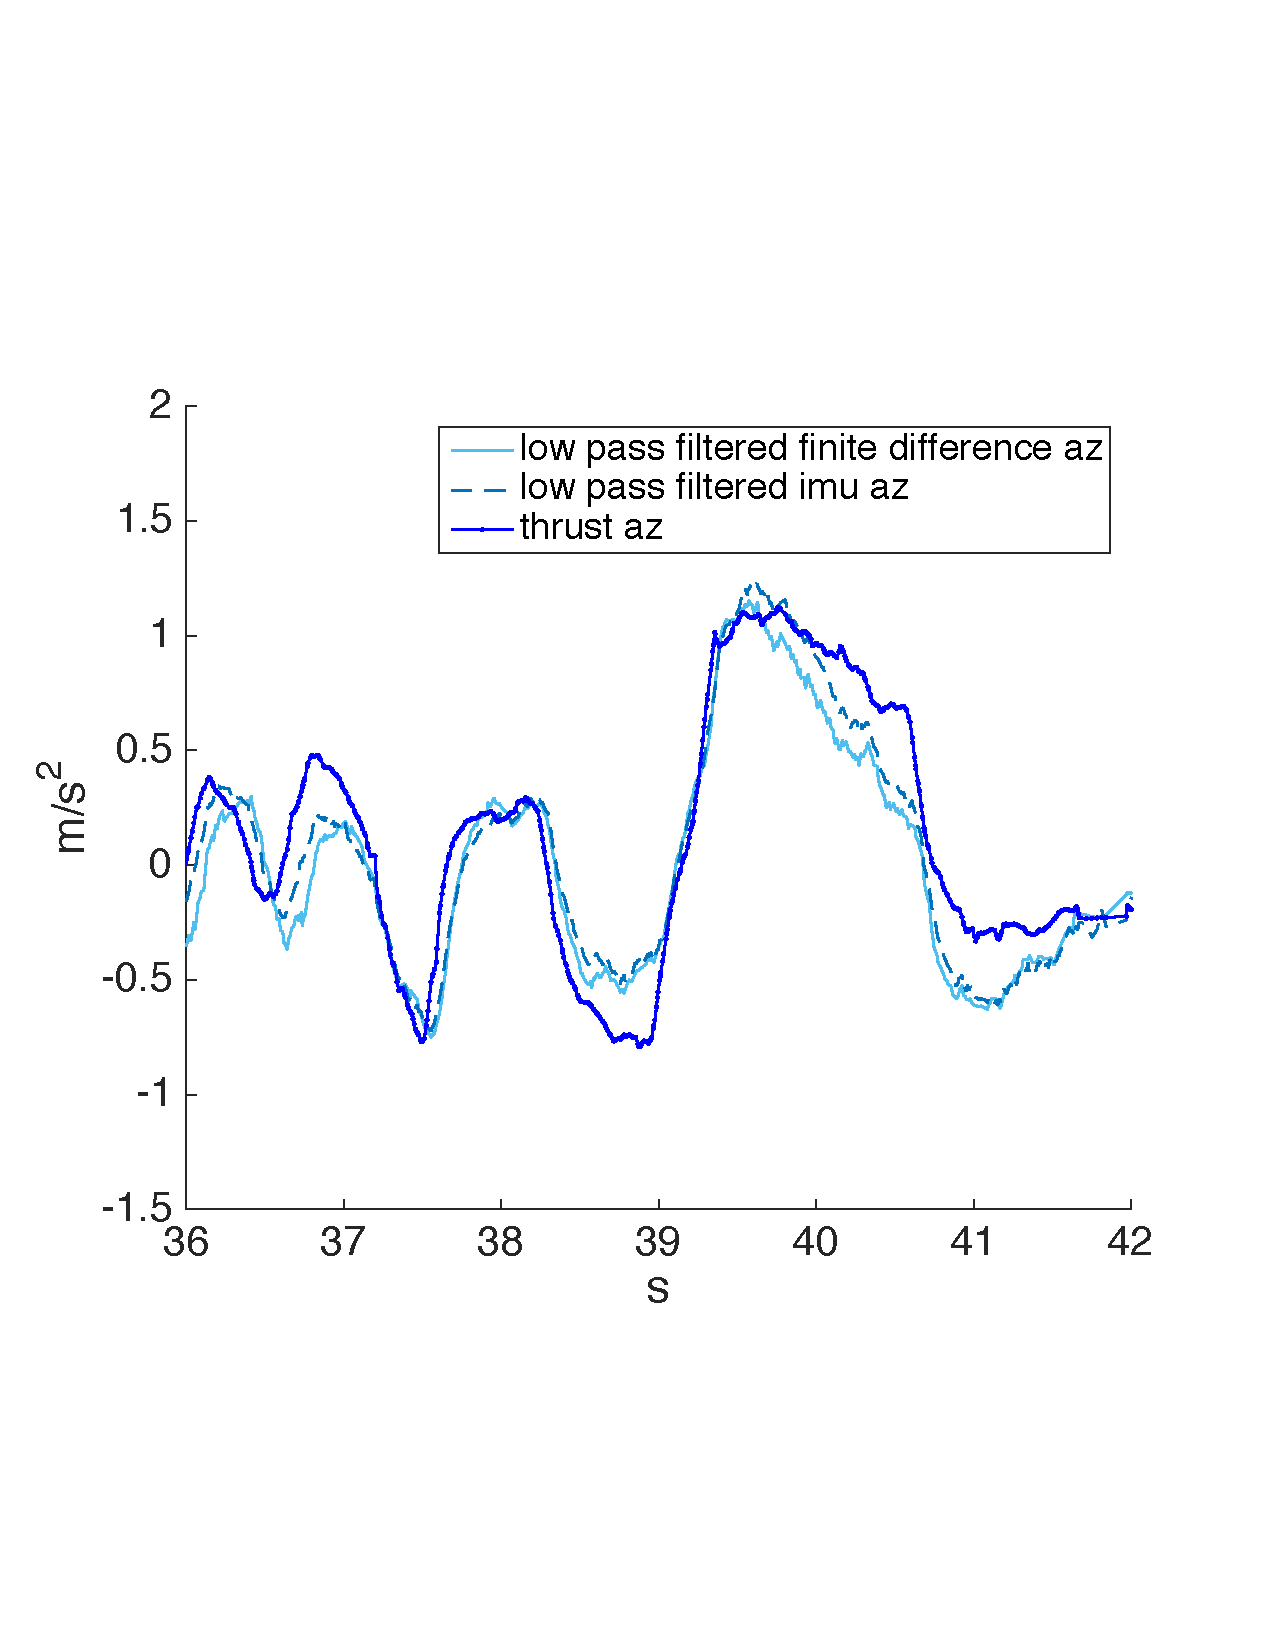
\includegraphics[width=\textwidth]{img/acceleration_mass_changed_filtered_z.pdf}
        \caption{Acceleration z axis filtered}
        \label{fig:comparison_accz_fil}
   \end{subfigure}
    \caption{Comparison between the accelerations calculate with the three different methods. On the left side the raw data without filtering IMU and finite difference measurements. On the right column the same data set, but with filtered version for IMU and finite difference.}
    \label{fig:comparison_acc}
\end{figure}

It is easy to notice that only the raw data from the thrust can be considered a good approximation of the acceleration, while the other two signals needs some filtering.\\
On the other side, the comparison of the filtered data has much more sense. In this case the data from IMU and finite difference are more smooth and can be used, but filtering the high frequencies we slow down the response of these signal and so cause a delay.\\

In the figure \ref{fig:comparison_acc} we can also notice that there is some offset between the three different approximations considering the same image, in particular in the z directions this difference it is very clear between the acceleration computed with the thrust and the other two methods.\\
This offset is more evident in the figure \ref{fig:comparison_acc_mass} where the right graph is the same figure \ref{fig:comparison_accz_fil}, while the left part is calculate with the same data set, but the mass of the quadrotor is modify by the $5\%$ from $515g$ to $545g$. This tiny modification is creating a big difference in the final acceleration.

\begin{figure}[!htbp]
 \centering   
  \begin{subfigure}[b]{0.45\textwidth}
     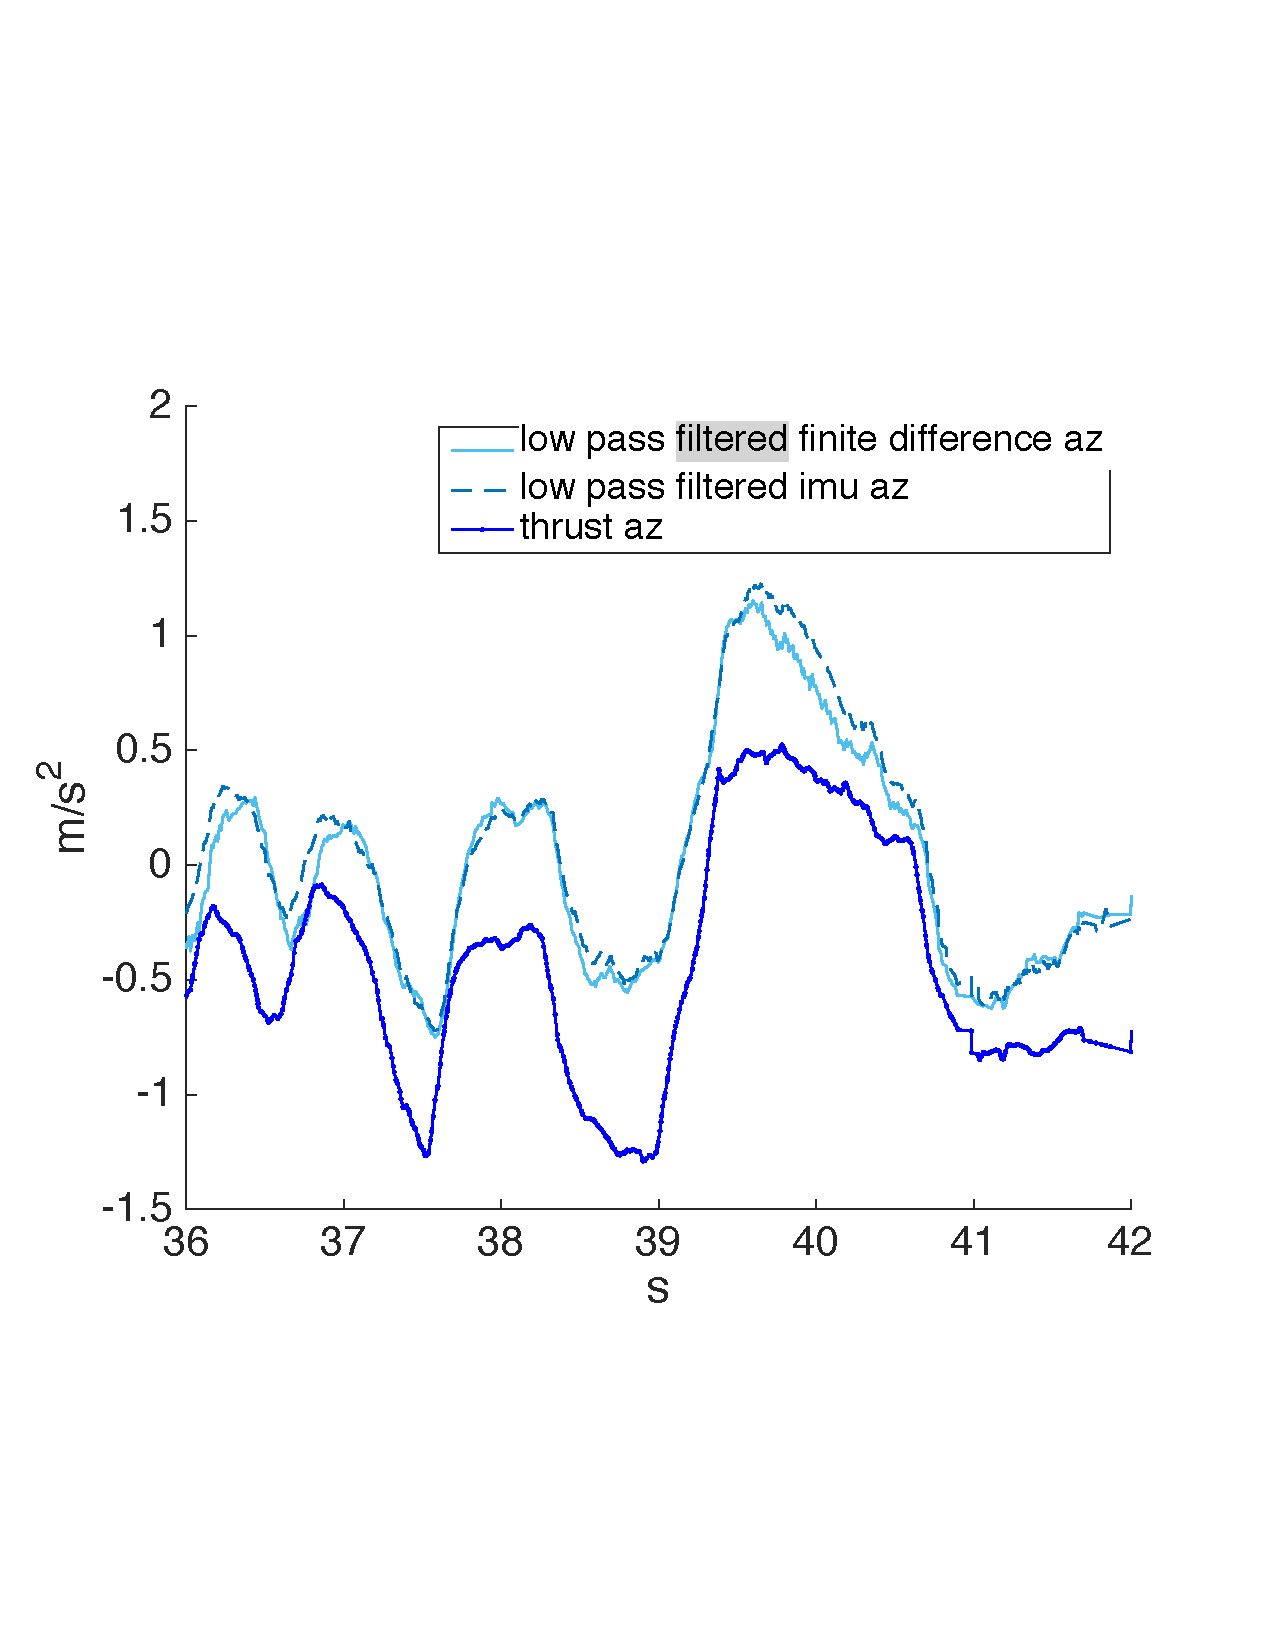
\includegraphics[width=\textwidth]{img/acceleration_mass_correct_filtered_z.pdf}
        \caption{Acceleration z axis filtered with real mass of 545g}
        \label{fig:comparison_accz_mass}
   \end{subfigure}
     \begin{subfigure}[b]{0.45\textwidth}
     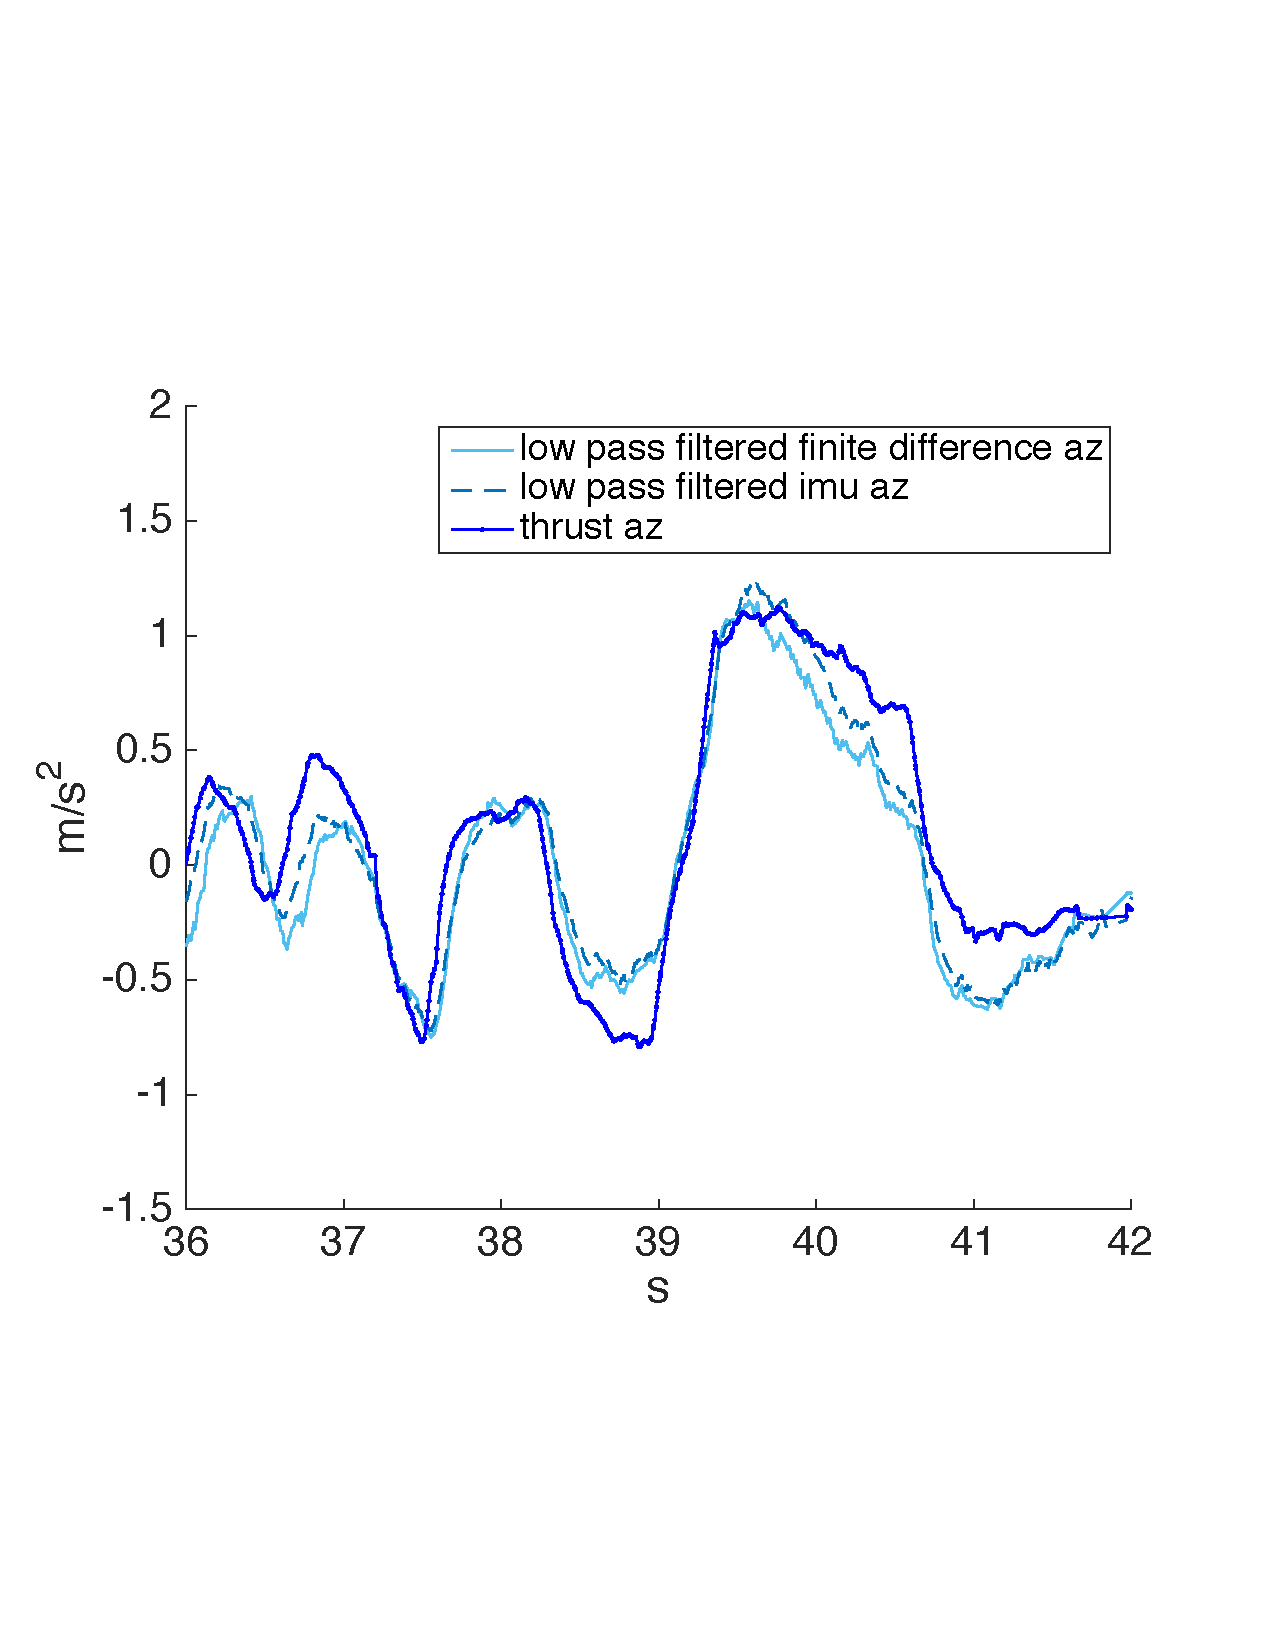
\includegraphics[width=\textwidth]{img/acceleration_mass_changed_filtered_z.pdf}
        \caption{Acceleration z axis filtered with modify mass of 515g}
        \label{fig:comparison_accz_fil_mass}
   \end{subfigure}
    \caption{Comparison between the accelerations calculate with the three different methods. On the left side accelerations calculate considering the real mass of 545g , on the right column considering 545g}
    \label{fig:comparison_acc_mass}
\end{figure}

Also in the other axis, if we change the mass, we can see that the acceleration estimation computed with the thrust shows an offset with respect to the other two signal.\\ This could be caused by a not precise estimation of the rotor fitness factors.\\

\section{Landing on a moving platform}
We also made different trials of the entire framework, in order to understand if all the pieces linked together are good enough to complete the task.\\
We have some videos in which we run the whole system from start to end with successful land on a moving platform.\\

In simulation we reached velocity of the moving platform up to $2\frac{m}{s}$, with landing rate of over $90\%$.
While in the real world we managed to achieve velocity of $1\frac{m}{s}$ for the platform. The main issues with higher velocity in the real world is that the state estimation starts to drift and the quadrotor we are using has hardware limitations that do not permit fast trajectory, so in the final stages of the state machine, the trajectory generator is not able to find feasible trajectories that bring the quadrotor on the platform. TODO

%\begin{figure}[h]
%   \centering
%   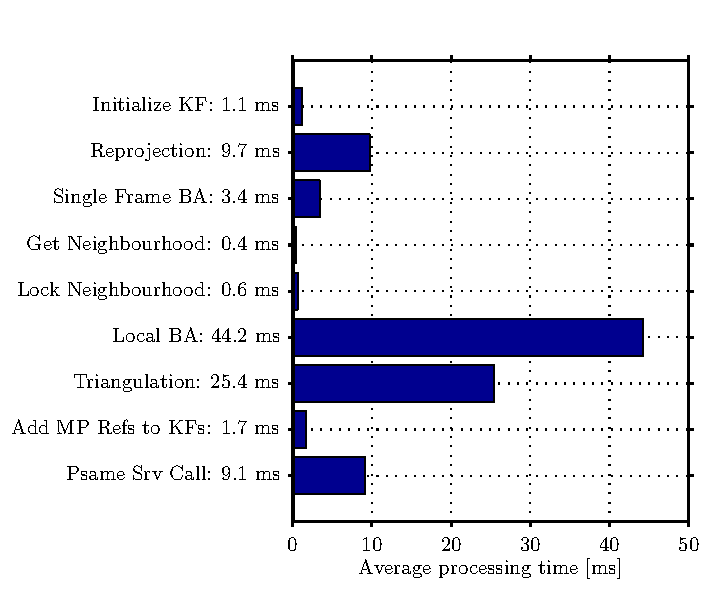
\includegraphics[width=0.75\textwidth]{img/processing_time.pdf}
%   \caption{Example of a figure.}
%   \label{img:timing}
%\end{figure}